%!TEX encoding = UTF-8 Unicode
% !TeX spellcheck = en_GB

%%%%%%%%%%%%%%%%%%%%%%%%%%%%%%%%%%%%%%
\chapter{ Higgs pair as a probe for light Yukawa couplings }\label{chap:lightyuk}
%%%%%%%%%%%%%%%%%%%%%%%%%%%%%%%%%%%%%%
The vast hierarchy of quark  ( and lepton) masses that we have seen in~ \autoref{smyukawa} poses one of the unsolved mysteries of the SM. As one might wonder whether the Higgs is Higgs is actually responsible for the quarks of first and second generation masses or there exist other physics that interplays with the Higgs. In fact, one of Weinberg's last papers was exactly addressing this question~\cite{Weinberg:2020zba}, in which he proposed that only the third generation fermions obtain their masses from Yukawa coupling, while the rest squire their masses via loop-level interactions. Despite his models being only illustrative, his paper indicates that even one of the pioneers of the SM theory was thinking about this mystery through the last year of his life !  \\
The pragmatic approach to unravelling this mystery , however, would be to measure directly the Higgs interaction with light fermions. Ideally, this would be via Higgs decay to first and second generation leptons. This is feasible for the muon case ~\cite{ATLAS:2020fzp,CMS:2020xwi}, challenging for the charm quarks~\cite{ATLAS-CONF-2021-021,ATLAS:2022ers,CMS:2019hve} but almost impossible with the current technologies for the electron~ \cite{Khachatryan:2014aep}, strange and first generation quarks. Although, lepton colliders might have potential for \emph{strange tagging}~\cite{Nakai:2020kuu}. The difficulties here is twofold, starting from the fact that the SM predict  these couplings to be extremely small effectually making these decay channels undetectable  even at few inverse attobarn luminosity. Secondly, even if NP would enhance the Higgs coupling to these fermions, the resolution of the LHC, would not be sufficient for efficient reconstruction of the Higgs from electron pairs, and it is not possible to distinguish up, down or gluon jets at the LHC and the untagged jets form an overwhelming background at any Hadron collider. This means that the search for these couplings ought to take a non-trivial path. Focusing on the production of the Higgs at the LHC, enhancements of light quark Yukawa couplings would open the tree-level quark anti-quark inhalation channel $\qqA$, which is enhanced  by the presence of light quarks in the PDF's. Moreover breaking the degeneracy amongst the strange up and down quarks, by having a \emph{production tagging} coming form the angular distributions of the PDF's for different quark flavours.  For sufficiently large enhancement of the light quark Yukawa couplings, this channel would even become dominant over the loop-induced gluon fusion, as~\autoref{fig:pphhvsh}. Working in an EFT paradigm, the $\qqA$ channel would contain a $hhq\bar q$ contact interaction illustrated in~\autoref{qqA_fd}, that would enhance the Higgs pair production even further than the single Higgs $\qqA $ making Higgs pair production more sensitive to light quark Yukawa enhancement, as the $\qqA$ production would become more dominant the di-Higgs ggF at lower values of light Yukawa enhancement as ~\autoref{fig:pphhvsh} shows. \\ Despite the ggF Higgs pair production channel in EFT containing a diagram with a contact  $hhq\bar q$  interaction shown in~\autoref{fig_ggf_diag}, the contribution is suppressed by the kinematic mass of the quarks appearing inside the loops, hence this channel's effect on enhancing the Higgs pair signal is negligible when light quarks Yukawa enhancement is considered. \\
\begin{figure}[!tb]
	\centering
	\begin{picture}(180,200)
		\put(-120,120){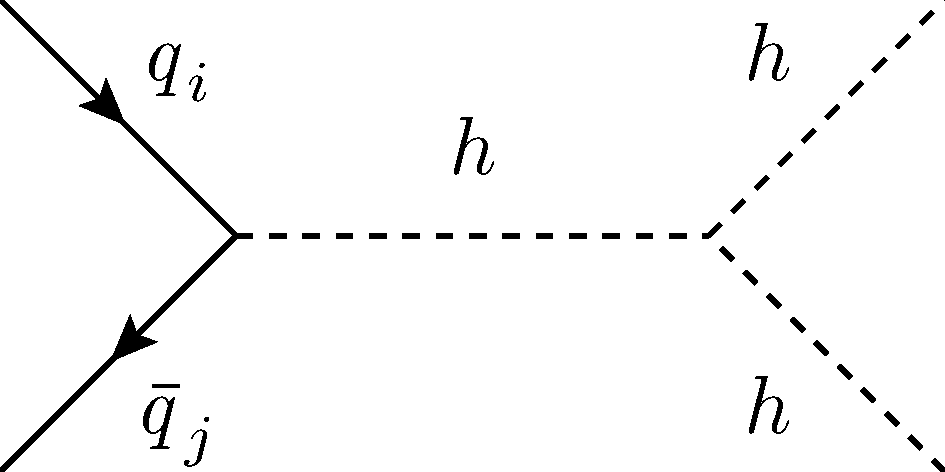
\includegraphics[scale =0.25]{./fig/qqh_higgs_prpg}}
		\put(20,120){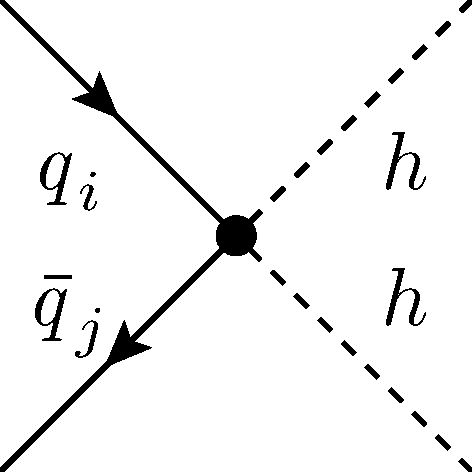
\includegraphics[scale = 0.25]{./fig/qqh_dim6}}
		\put(110,110){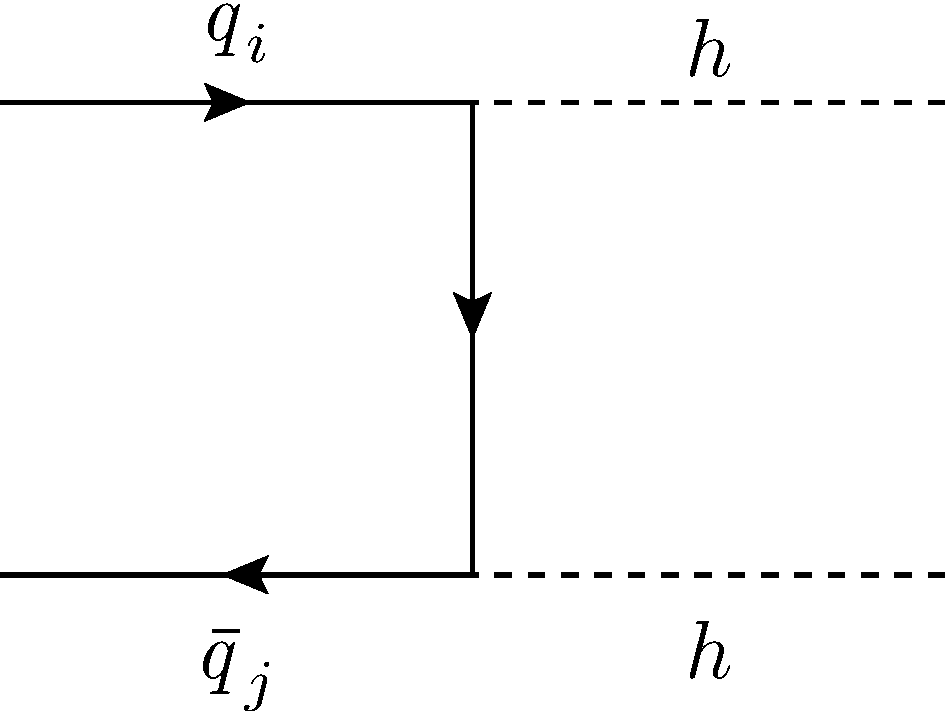
\includegraphics[scale =0.21]{./fig/qqh_tchannel}}
		\put(230,145 ){{\large+ crossed} }
	\end{picture}
	\vspace*{-4cm}
	\caption{ Feynman diagrams for the $\qqA$ Higgs pair production in the EFF paradigm. The middle diagram shows a contact $hh q\bar q$ interaction, that contributes to significant enhancement of this channel compared to its single Higgs counterpart. }
	\label{qqA_fd}
\end{figure}
\begin{figure}[t]
	\centering
	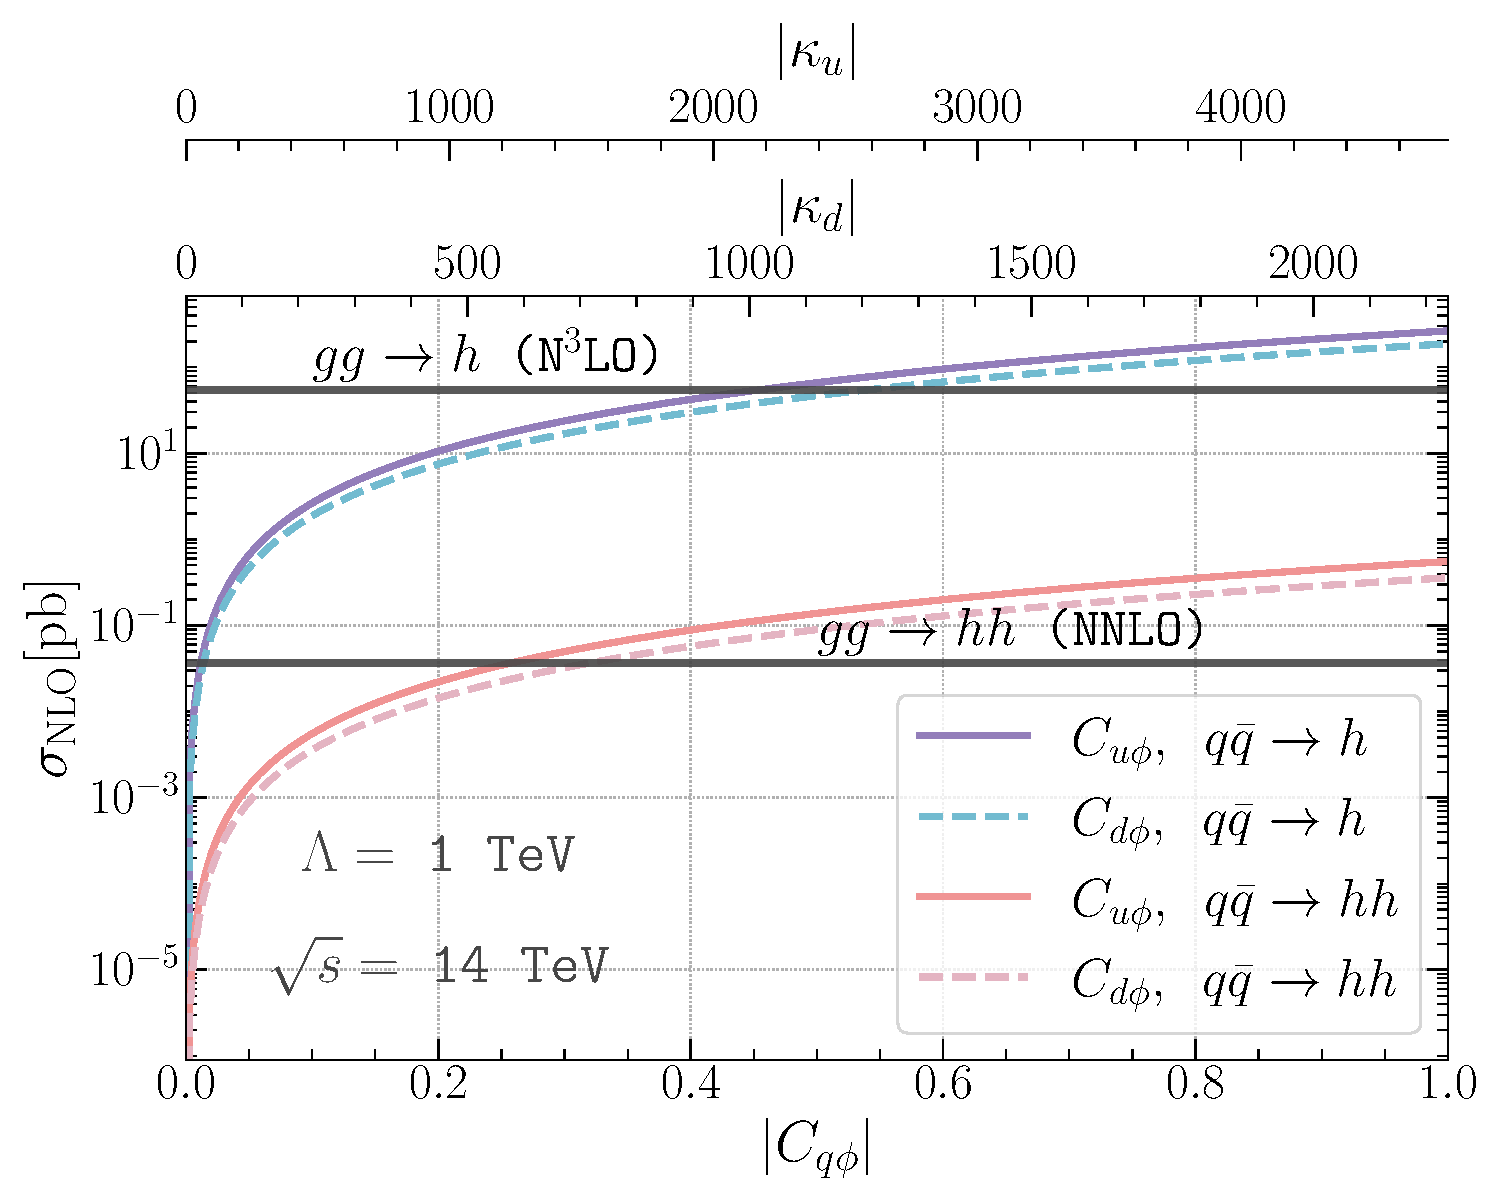
\includegraphics[width=0.75\textwidth]{fig/pph_hh_14Tev.pdf}
	\caption{\it The production cross-section of single Higgs and di-Higgs at $14$ TeV from the quark anti-quark annihilation $q\bar{q}A$ as a function of the Wilson coefficients $C_{u\phi}$ and $C_{d\phi}$ versus the SM gluon fusion cross-sections (the horizontal solid line for $gg \to h$ and the dashed-dotted one for $gg \to hh$). One can observe that for values of $C_{u\phi}=0.22\, (0.43)$ and $C_{d\phi}=0.26\, (0.47)$ the $q\bar{q}A$ channel becomes the dominant di-Higgs (single Higgs) production channel. The UV scale is set to $\Lambda = 1$ TeV. }
	\label{fig:pphhvsh}
\end{figure} 
\begin{figure}[!hb]
	\centering
	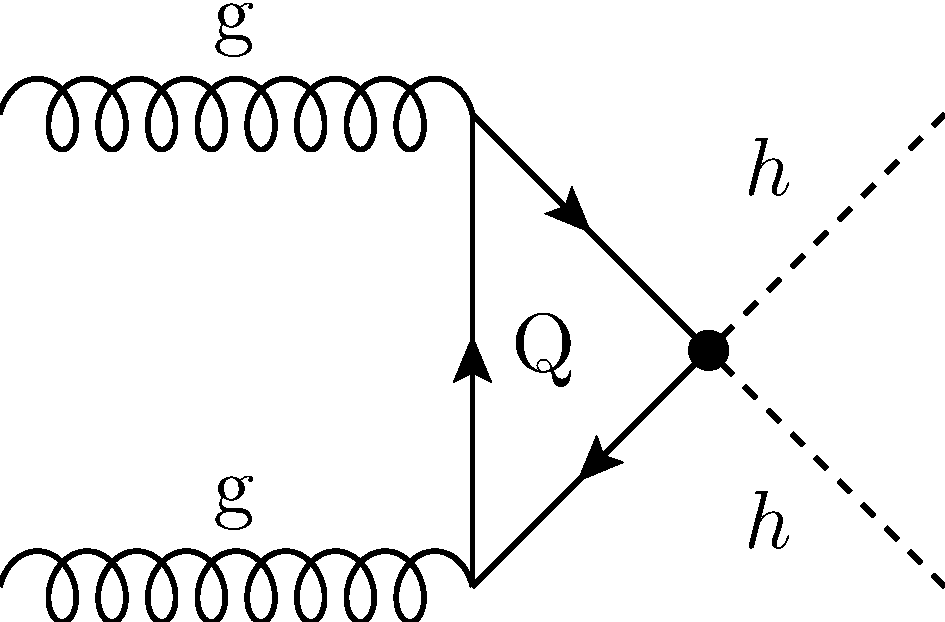
\includegraphics[width = 0.25\textwidth]{./fig/ggfdim6}
	\caption{The new diagram for ggF emerging from the $hh q \bar q$ coupling stemming from an effective dim-6 operator.}
	\label{fig_ggf_diag}
\end{figure}
This chapter aims to exploit the potential for Higgs pair production as a direct measurement channel for light quark Yukawa. Focusing on the first generation quarks.  I will start by introducing the inclusion of light quark couplings to the Higgs in the EFT framework in~\autoref{sec:EFTlightyuk}. Then the NLO QCD calculation of the $\qqA$ channel will be shown in~\autoref{sec:qqHH}. \autoref{sec:cutbasedly} will outline a cut-based analysis of the di-Higgs final state $ b \bar b \gamma \gamma$ in order to estimate the sensitivity of this channel for the HL-LHC. Later, in~\autoref{sec:mlanalysisly} an optimised approach for enhancing the sensitivity based on interpretable machine learning will be showcased. The results of both analysis techniques will be discussed and compared in ~\autoref{sec:resultsly} While in ~\autoref{sec:comparetoothers} I will overview  the other searches for light Yukawa couplings comparing it the Higgs pair production expected sensitivity. This chapter will be concluded in~\autoref{sec:concly}. \\ The cut-based analysis has been published in~\cite{Alasfar:2019pmn}, while the interpretable machine-learning one is an undergoing project with \\ The analysis of the final state $b \bar b \gamma \gamma$ for the HL-LHC simulated events details can be either found in the aforementioned paper or appendix Cut-based analysis and fit results on the second generation quarks are found in the appendix. \la{add this later}
%%%%%%%%%%%%%%%%%%%%%%%%%%%%%%%%%%%%%%%%%%%%%%%%%%
\section{Effective Field Theory of light Yukawa couplings\label{sec:EFTlightyuk}}
%%%%%%%%%%%%%%%%%%%%%%%%%%%%%%%%%%%%%%%%%%%%%%%%%%
Including the flavour indices~$ij$ of the SMEFT operators introduced in refs.~\cite{Grzadkowski:2010es,Contino:2013kra} and~\autoref{chap:HiggsEFT}, we would get light quark -Higgs coupling enhancement from the operators
\begin{equation}
	\Delta \mathcal{L}_{y}=\frac{\phi^{\dagger}\phi}{\Lambda^2}\left( C_{u \phi}^{ij} \bar{Q}_L^i \tilde{\phi} u_R^j + C_{d \phi}^{ij} \bar{Q}_L^i \phi d_R^j +h.c.\right)\,,
	\label{eq:EFTop}
\end{equation}
  The mass matrices of the up- and down-type quarks obtained from the Yukawa and the new SMEFT coupling are
 %
 \begin{align}
 	M^u_{ij} =& \frac{v}{\sqrt{2}} \left( y^u_{ij}-\frac{1}{2} (C_{u\phi})_{ij}\frac{v^2}{\Lambda^2}\right)\,,\nonumber\\
 	M^d_{ij} =& \frac{v}{\sqrt{2}} \left( y^d_{ij}-\frac{1}{2} (C_{d\phi})_{ij}\frac{v^2}{\Lambda^2}\right)\,, \label{eq:mass}
 \end{align}
where $y^q_{ij}$ are the SM Yukawa matrix elements introduced in eq.~\eqref{lag-yuk}. Since the quark masses are measured quantities, one would naturally rotate to the mass basis using bi-unitary transformation represented by the matrices ~$ \mathcal{V}_q, \mathcal{U}_q$, like in the SM. The Wilson coefficients matrix elements in the flavour space in the mass basis can be written as
\begin{equation}
	\tilde{C}_{q \phi}^{ij}= \left(\mathcal{V}_{q}\right)^*_{ni}C^{nm}_{q\phi}\left( \mathcal U_{q}\right)_{mj}\, , \; \; \; \;  \text{with } \;\;\;\;\; q = u,d\, .
\end{equation}
n order to match these Wilson coefficients to Higgs couplings to quarks, we use the Lagrangian operator describing these couplings
\begin{equation}
	\mathcal{L}\supset g_{h\bar{q}_i q_j}\bar{q}_i q_j h + g_{h\bar{q}_i q_j}\bar{q}_i q_j h^2
\end{equation}
Then the matching results in identifying the SMEFT couplings of Higgs and quarks
\begin{equation}
	g_{h\bar{q}_i q_j} := \quad \frac{m_{q_i}}{v}\delta_{ij}-\frac{v^2}{\Lambda^2} \frac{	\tilde{C}_{q \phi}^{ij}}{\sqrt{2}}\,, \quad \quad \quad \quad \quad g_{h h\bar{q}_i q_j} := \quad -\frac{3}{2\sqrt{2}}\frac{v}{\Lambda^2}	\tilde{C}_{q \phi}^{ij}\,. \label{eq:couplingsEFT}
\end{equation}
We observe that, in the general case, we will be having non-diagonal couplings. However, such couplings are strongly constraint by flavour observables , particularly neutral meson mixing~\cite{Blankenburg:2012ex}.
\begin{equation}
|\tilde{C}_{q\phi}^{12}| \lesssim 10^{-5} \Lambda^2/v^2| \quad \quad  \quad \quad | \tilde{C}_{d\phi}^{13/23}| \lesssim 10^{-4} \Lambda^2/v^2
	\end{equation}
 Due to these strong constraints, it is typical to consider SMEFT with minimal flavour violation~(MFV)~\cite{DAmbrosio:2002vsn}, in which the SM Yukawa matrices $y_q^{ij}$ are the only spurions breaking the global $SU(3)_Q \otimes SU(3)_U \otimes SU(3)_D \to U^6(1)$ flavour symmetry. This would imply that the Wilson coefficients matrices in the mass basis are simultaneously diagonalisable with the SM Yukawa matrices. This make the Wilson coefficients  maintain the hierarchy of the couplings seen in the SM, thus MFV is not a viable scheme when one wants to consider significant enhancements to the couplings for first and second generations, but keep the third generation couplings unchanged. \\ In order to bypass the constraints of MFV and yet avoid flavour changing neutral currents~(FCNC) that are prohibited by flavour observables, one needs to turn to  flavour alignment~\cite{Pich:2009sp,Pich:2010ic} or its generalisation aligned flavour violation~(AFV)~\cite{Egana-Ugrinovic:2018znw} . \\ 
 With flavour alignment, the NP flavour parameters~(here the Wilson coefficients) are aligned with the SM Yukawa, such that both can be simultaneously diagonalised, hence preventing tree-level FCNCs. But unlike MFV, the constraint on making these new parameters proportional to the SM Yukawas is lifted.  This would induce radiative FCNCs, as this formalism in unstable under quantum corrections ~\cite{Ferreira:2010xe,Jung:2010ik,Botella:2015yfa}. This alignment breaking would not be seen in the SMEFT, but rather when UV-complete models are considered. AFV resolves this instability, by ensuring that any NP spurion breaking the flavour symmetry will transform trivially under the quark phases transformations $ U^6(1)$, keeping the CKM matrix as the only flavour object that has non-trivial transformations. Thereby the CKM will have physical flavour changing currents as well as a $\mathcal{CP}$-violating phase. This constraint on the NP flavour spurions $k_q$, allows them to be written as a series in powers of the CKM matrix, known as the alignment expansion
 \begin{align}
 	k_u &= K_{0,u}+ K_{1,u} V^*_{CKM} K_{2,u} V^T_{CKM} K_{3,u} + \mathcal O(V^4_{CKM})+ \dots,  \\
 	(k_d)^\dagger&=K_{0,d}+ K_{1,d} V^T_{CKM} K_{2,d} V^*_{CKM} K_{3,d} + \mathcal O(V^4_{CKM}) + \dots,
 	\label{eqK}
 \end{align}
 where $K_{i,u}$ and $K_{i,d}$ are complex $3\times3$ diagonal matrices invariant under flavour transformations. This formalism is stable under renormalisation group evolution as any linear combinations or tensor product of the spurions will remain flavour aligned. \\
 For simplicity, I shall only consider the first term in the alignment expansion, such that only diagonal $C_{q\phi}$ are investigated, as the other terms are already CKM-suppressed and not of particular phenomenological interest.  With this in mind, and using the translation between SMEFT and $\kappa$-formalism discussed in~\autoref{eftkappa}, it is possible to identify the couplings in SMEFT with the $\kappa$'s
\begin{equation}
	g_{h\bar{q}_i q_i} =\kappa_q g_{h\bar{q}_i q_i}^{\text{SM}} \,, \quad \quad \quad \quad \quad g_{h h\bar{q}_i q_i}= - \frac{3}{2}\frac{1-\kappa_q}{v}g_{h\bar{q}_i q_i}^{\text{SM}} \,,
	\label{eq:def_kappa}
\end{equation}
in a slight abuse of language of the $\kappa$-framework used often in experimental analyses, as the $hhq \bar q$ coupling also depends on the light quarks coupling modifier $\kappa_q$. 
\par
Higgs pair production offers an extra advantage for probing light Yukawa interactions, as it is particularly sensitive to the $hh q\bar q$ interaction, one could also consider the non-linear HEFT/EWChL, by extending it to include Wilson coefficients $c_q$ and $c_{qq}$ for the first and second generation quarks, in analogy to ones defined for the top quark in eq.~\eqref{eq:coupl_def}~ \cite{Contino:2010mh}.
%%%%%%%%%%%%%%%%%%%%%%%%%%%%%%%%%%%%%%%%%%%%%%%%%%
\section{Higgs pair production and Higgs decays with modified light Yukawa couplings \label{sec:qqHH}}
%%%%%%%%%%%%%%%%%%%%%%%%%%%%%%%%%%%%%%%%%%%%%%%
In this section we will describe how the Higgs pair production process for modified light quark Yukawa couplings is affected.
While in the SM Higgs pair production is dominantly mediated by gluons fusing into a heavy quark loop coupling to the Higgs boson, for large first and second generation quark Yukawa couplings
also quark annihilation becomes relevant.
For a phenomenological analysis we also need to take into account the Higgs boson decays, which we describe in the last part of the section.
\subsection{Higgs pair production via gluon fusion \label{sec:ggFly}}

For our analysis, we have calculated the $ \sqrt{s} = 14$ \text{TeV}  LO ggF inclusive cross section and distributions with modified light Yukawa couplings by including the light quark loops and the coupling $hh q \bar q$ shown in fig.~\ref{fig_ggf_diag}.

The calculation was carried out using a private FORTRAN implementation of the LO cross section utilising the \texttt{VEGAS} integration algorithm, and NNPDF30 parton distribution functions~(PDF's)\cite{Ball:2017nwa} implemented via the \texttt{LHAPDF-6} package \cite{Buckley:2014ana}. For the one-loop integrals appearing in the form factors of the box and triangle diagrams, we have used the \textsc{Collier} library~\cite{Denner:2014gla} to ensure numerical stability of the loop integral calculation for massless quarks inside the loops.

\subsubsection{Results}
For comparison of the results with modified Yukawa couplings with the SM results, we define as a benchmark point the case where all first and second generation quark Yukawa couplings are scaled to the SM bottom Yukawa coupling, which we will refer to in plots and tables as $g_{hq \bar q} = g_{h b \bar b}^{\SM}$. This means we scale the Yukawa couplings by $\kappa_q=g_{h\bar{q}q}/g_{h\bar q q}^{\SM}$ with
\begin{equation}
	\kappa_u=  1879\,, \hspace*{0.5cm} \kappa_d= 889 \,, \hspace*{0.5cm}\kappa_s= 44\,, \hspace*{0.5cm} \kappa_c =3.3\,, \label{eq:fitbounds}
\end{equation}
and use only flavour-diagonal modifications of the quark Yukawa couplings.
This benchmark is inspired by ref.~\cite{Bar-Shalom:2018rjs}.

From the distributions it is evident, that the change of the ggF process in the presence of enhanced light Yukawa couplings is quite small. The reason is that the box contribution which is the major part of the cross section has two fermion coupling insertions and hence is strongly suppressed for all the light quarks with respect to the top quark loop diagrams. The bottom quark contribution to the ggF process in the SM is less than 1\% and comes mainly from the triangle diagram, so adding several contributions from similar size does not change the cross section by much. Also the new diagrams (\textit{cf.}~fig.~\ref{fig_ggf_diag}) are suppressed compared to the box diagrams of the top quark.
In the presence of enhanced light quark Yukawa couplings the Higgs boson pair can though be directly produced by quark annihilation. We turn to discuss this process in the next part. In the meanwhile we can conclude that for the ggF process we can improve on the LO predictions by using SM $K$-factors and that the effects of light Yukawa coupling modifications for the ggF process are small for the still allowed modifications.
%%%%%%%%%%%%%%%%%%%%%%%%%%%%%%%
\subsection{Higgs pair production via quark anti-quark annihilation}
If the Yukawa couplings of the light quark generations are sufficiently increased, the Higgs bosons will be produced directly from the constituents of the proton with a sizeable rate. The quark anti-quark annihilation (qqA) process becomes then relevant for Higgs pair production.
The qqA process has four Feynman diagrams shown in the fig.~\ref{qqA_fd}.
%%
The differential cross section given by
\begin{align}
	\frac{d \hat \sigma_{q_i\bar{q}_j}}{d \hat t} &= \frac{1}{16 \pi}\, \frac{1}{12  \hat{s}} \bigg[ \left| 2  g_{hh q_i \bar q_j} + \frac{g_{hhh}\, g_{h q_i \bar q_j}}{\hat{s}-m_h^2-im_h\Gamma_h}\right|^2+ \mathcal{O}(g_{h q_i \bar q_j}^4) \bigg].
	\label{sigmaqqa}
\end{align}

We neglect here the $\hat{t}$ and $\hat{u}$ channel diagrams, as their contribution is typically only $\sim 0.1 \%$ of the total cross section.

The hadronic cross section is then obtained by
\begin{equation}
	\sigma_{\mathrm{hadronic}} =  \int_{\tau_0}^1 d\tau \int_{\hat{t}_-}^{\hat{t}_+} d\hat{t} \sum_{i,j} \frac{d\mathcal{L}^{q_i\bar{q}_j}}{d\tau}\frac{ d\hat \sigma_{q_i\bar{q}_j}}{d \hat t}\,, \label{eq:sigmahadron}
\end{equation}
with $ \tau_0= 4\, m_h^2/s$, $\hat{s}=\tau s$ and
\begin{equation}
	\hat{t}_{\pm}=m_h^2-\frac{\hat{s}(1\mp \beta)}{2} \quad\quad \text{and}\quad \quad \beta=\sqrt{1-\frac{4 m_h^2}{\hat{s}}}\,.
\end{equation}
The parton luminosity is given by
\begin{equation}
	\frac{d{\cal L}^{q_i \bar q_j}}{d\tau} = \int_\tau ^1 \frac{dx}{x} \,\left[  f_{q_i}(x/\tau,\mu_F^2) f_{\bar{q}_j}(x,\mu_F^2) + \,f_{\bar{q}_j}(x/\tau,\mu_F^2) f_{q_i}(x,\mu_F^2)\right]\,.
\end{equation}
We neglected all the kinematic masses in accordance with the 5-flavour scheme of the PDFs while the coupling of the Higgs boson to the light quarks (for flavour diagonal couplings) is
\begin{equation}
	g_{hq_i\bar{q}_j}=\frac{m^{\bar{MS}}_q(\mu_R)}{v}  \kappa_q \delta_{ij}\,,
\end{equation}
and analogously for the $g_{hhq_i\bar{q}_j}$ coupling.\footnote{We note that there is no inconsistency with such an assumption since in scenarios of modified Yukawa couplings, the masses of the quarks need not to be generated by electroweak symmetry breaking.}
%
\subsubsection{NLO QCD correction \label{sec:qqA_NLO}}
%
Since NLO QCD corrections are sizeable, we will take them into account in our analysis. For this purpose, we will detail here how we obtained them.
Since the $\hat{t}$ and $\hat{u}$ channel diagrams are strongly suppressed we can take the NLO QCD corrections over from $ b \bar b \to h$ in the 5-flavour scheme~\cite{Dicus:1998hs, Balazs:1998sb, Harlander:2003ai}\footnote{Note that the NLO and NNLO QCD corrections for $b\bar{b}hh$ have been given in \cite{Dawson:2006dm,  H:2018hqz}.}  by some adjustments taking into account the modified LO cross section and the different kinematics of the process.
The Feynman diagrams at NLO QCD are shown in fig.~\ref{qqA_nlo}.
%%
\begin{figure}[!t]
	\centering
	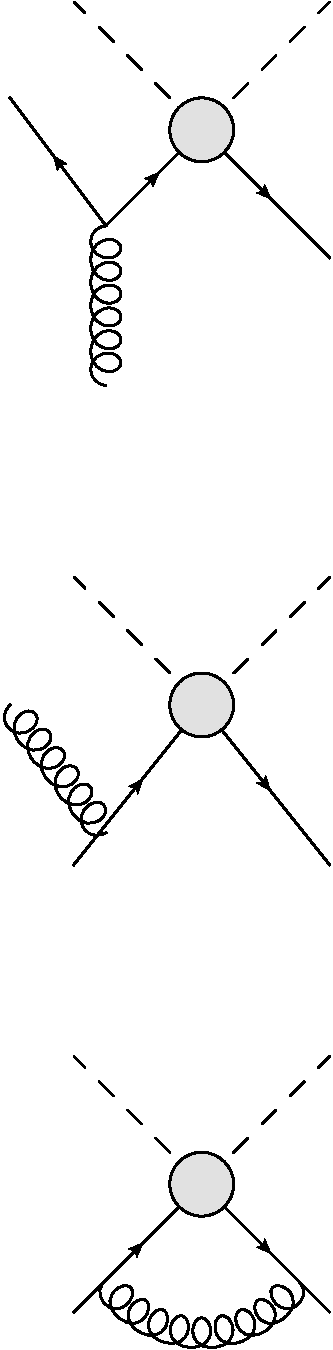
\includegraphics[width = 0.20\textwidth, angle = -90]{./fig/qqbar_hh_nlo.pdf}
	\caption{Generic form of the QCD corrections of order $\mathcal O(\alpha_s)$ to the qqA Higgs pair production. }
	\label{qqA_nlo}
\end{figure}
%%
For convenience and for making our adjustments explicit we report here the formulae from \cite{Spira:2016ztx}
%%
\begin{subequations}
	\begin{eqnarray}
			\sigma(q\bar q\to h) & = & \sigma_{LO} + \Delta\sigma_{q\bar q} +
			\Delta\sigma_{qg}  \\
			\Delta\sigma_{q\bar q} & = & \frac{\alpha_s(\mu_R)}{\pi} \int_{\tau_0}^1
			d\tau \sum_q \frac{d{\cal L}^{q\bar q}}{d\tau} ~\int_\tau^1 dz~\hat{\sigma}_{LO}(Q^2=z\tau s)~\omega_{q\bar
					q}(z)  \\
			\Delta\sigma_{qg} & = & \frac{\alpha_s(\mu_R)}{\pi} \int_{\tau_0}^1 d\tau
			\sum_{q,\bar q} \frac{d{\cal L}^{qg}}{d\tau}~\int_\tau^1 dz~\hat{\sigma}_{LO}(Q^2=z\tau s)~\omega_{qg}(z)
		\end{eqnarray}
\end{subequations}
and
\begin{equation}
	\hat{\sigma}_{LO}(Q^2)= \int_{\hat{t}_-}^{\hat{t}_+} \frac{ d\hat \sigma_{q_i\bar{q}_j}}{d \hat t}
\end{equation}
%%
with $z=\tau_0/\tau$, $\sigma_{LO}=\sigma_{\mathrm{hadronic}}$ of eq.~\eqref{eq:sigmahadron}, and the $\omega$ factors are given by \\
%%
\begin{subequations}
	\begin{eqnarray}
			\omega_{q\bar q}(z) & = & -P_{qq}(z) \ln \frac{\mu_F^2}{\tau s}
			+ \frac{4}{3}\left\{ \left(2\zeta_2-1 +
			\frac{3}{2}\ln\frac{\mu_R^2}{M_{hh}^2} \right)\delta(1-z)  \right. \\ &+ & \left.  (1+z^2) \left[
			2 {\cal D}_1(z) - \frac{\ln z}{1-z} \right] + 1-z \right\} \nonumber \,, \\
			\omega_{qg}(z) & = & -\frac{1}{2} P_{qg}(z) \ln \left(
			\frac{\mu_F^2}{(1-z)^2 \tau s} \right) - \frac{1}{8}(1-z)(3-7z)\,,
		\end{eqnarray}
\end{subequations}
%%
with $ \zeta_2 = \frac{\pi^2}{6}$.
The Altarelli Parisi splitting functions $ P_{qq}(z)$ and $ P_{qg}(z)$~\cite{gribov1972deep,Altarelli:1977zs,Dokshitzer:1977sg} are given by
\begin{subequations}
	\begin{align}
			P_{qq}(z) & = \frac{4}{3} \, \left[2{\cal D}_0(z)-1-z+\frac{3}{2}\, \delta(1-z)\right],  \\
			P_{qg} &= \frac{1}{2}\, \left[  z^2+(1-z)^2\right],
		\end{align}
\end{subequations}
and the `plus' distribution is
\begin{equation}
	{\cal D}_n(z) := \left(\frac{\ln(1-z)^n}{1-z} \right)_+.
\end{equation}
We have chosen the renormalisation scale $ \mu_R = M_{hh}$ and the factorisation scale $ \mu_F= M_{hh}/4$, as central values.
We define the NLO $K$-factor, as
\begin{equation}
	K_{NLO}=\frac{\sigma_{NLO}}{\sigma_{LO}} = 1.28 \pm 0.02\,,
\end{equation}
with the error denoting the theoretical uncertainty.
The $K$-factor does not depend on the scaling of the couplings, nor the flavour of the initial $q \bar q$ since the LO cross section factors out (with exception of the different integration in the real contributions).

\subsubsection{Results}
While in the SM, the contribution from quark annihilation to a Higgs boson pair is below $0.11$ fb at NLO, it scales like $ \sim \kappa_q^2 m_q^2/v^4$, dominated by the $hh \bar q q$ diagram as can be seen from eq.~\eqref{sigmaqqa}, hence showing significant enhancement for enhanced Yukawa couplings.
For our benchmark scenario $(g_{hq \bar q} = g_{h b \bar b}^{\SM})$ we find for the cross section
\begin{equation}
	\sigma^{qqA}_{NLO}= 284 \pm 25 \text{ fb}\,,
\end{equation}
and therefore a significantly larger cross section as for the ggF process.
\begin{figure}[!t]
	\centering
	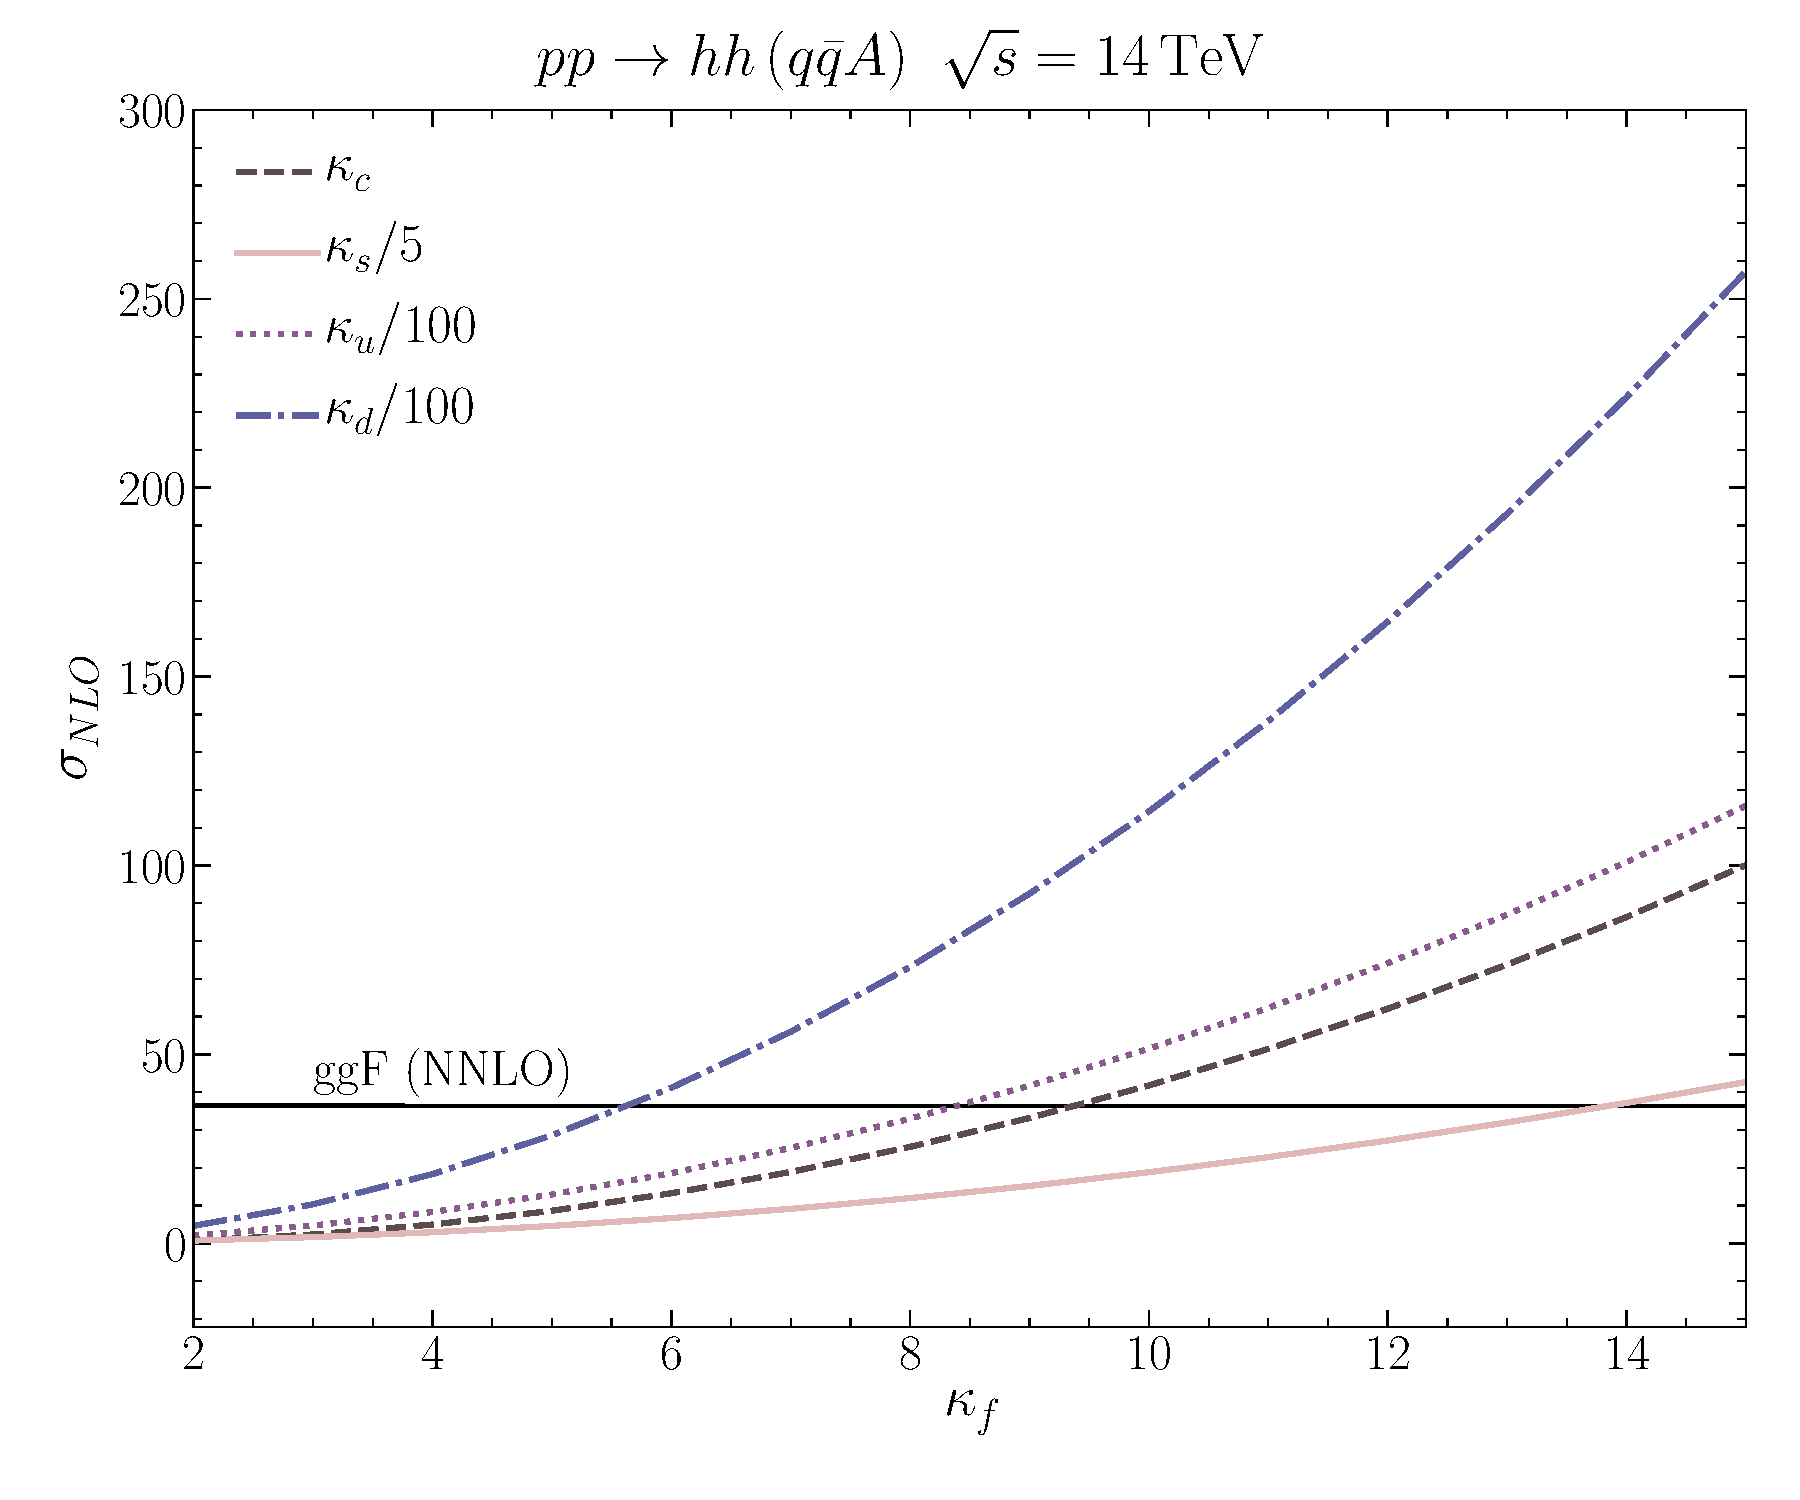
\includegraphics[width = 0.75\textwidth]{./fig/xs_qqa_kf}
	\caption{The NLO cross section for the qqA process for different scalings of the quark Yukawa couplings. The solid black line shows the NNLO ggF process width rescaled charm Yukawa coupling, whose effect though is unrecognisable in the plot. }
	\label{qqA_ggF}
\end{figure}
In fig.~\ref{qqA_ggF} we compare the ggF process (black line) for rescaled charm coupling to the Higgs boson(s) with the qqA process for different scalings of the light quark Yukawa couplings  (different coloured, dashed, dotted solid and dashed dotted lines).
We find that for sufficiently large scaling of the Yukawa couplings still allowed by current data, qqA can be even  the dominant di-Higgs production channel. Note that in the figure we scale the Yukawa couplings for the different quark mass eigenstates differently. For the up and down quark Yukawa coupling the scaling is the same, hence the effect from rescaling the down Yukawa coupling is larger even though the up quark is more abundant in the proton. The plot shows nicely for which values of the coupling modifications the qqA process surpasses ggF. \\
We would also like to give a qualitative argument for the dominance of qqA for large $\kappa_q$.
The dominant term for the qqA comes from the $hh q \bar q$ vertex diagram, such that the qqA cross section behaves for large values of $\kappa$ as (assuming that $ \sigma^{qqA}_{SM}\sim 0 $)
\begin{equation}
	(\sigma^{qqA}-\sigma^{qqA}_{SM}) \sim  g_{hh q \bar q}^2 \sim v^{-4}\,{m_q^2\,\kappa_q^2}.
\end{equation}
The ggF cross section instead gets contributions from light quark loops from  the diagram in fig.~\ref{fig_ggf_diag} interfering with top quark loops in the triangle SM diagram,  leading to a scaling of
\begin{equation}
	(\sigma^{ggF} - \sigma^{ggF}_{SM} ) \sim  \kappa_q\, \frac{m_q^2}{ v^2\,M_{hh}^2}\,\ln^2{\left(\frac{M_{hh}}{m_q}\right)}\,.
\end{equation}
Taking the ratio we get
\begin{equation}
	\frac{(\sigma^{qqA}-\sigma^{qqA}_{SM})}{(\sigma^{ggF} - \sigma^{ggF}_{SM} )} \sim  \frac{\kappa_q}{ v^2\left(\frac{
					\ln^2{\left(\frac{M_{hh}}{m_q}\right)}}{M_{hh}^2}\right)}\,.
\end{equation}
This ratio approaches one (neglecting effects from different PDFs) when
\begin{equation}
	\kappa_q^{qqA = ggF} \sim  \frac{v^2\,\ln^2{\left(\frac{M_{hh}}{m_q}\right)}}{M_{hh}^2}\,.
\end{equation}
Using this order of magnitude estimate, we see that  the two cross sections are roughly equal if $\kappa_c^{qqA = ggF} \sim 1$, $\kappa_s^{qqA = ggF} \sim 10$ and $\kappa_u^{qqA = ggF} \sim \kappa_d^{qqA = ggF} \sim 10^3$.
The actual values of $\kappa_q^{qqA = ggF}$ can be read from fig.~\ref{qqA_ggF}. We observe that $ \kappa_q^{qqA = ggF}$ values  are not yet excluded, particularly for the first family.
\par
In fig.~\ref{qqA_dsigdmhh} we show the di-Higgs invariant mass  normalised differential cross section distributions for the $g_{hq \bar q} = g_{h b \bar b}^{\SM}$ benchmark point at NLO compared to the NNLO SM ggF cross section extracted from~\cite{Grazzini:2018bsd}. We notice a considerable shape difference, with shifted peak to the left, and a larger tail. This will allow us later on to use kinematical information to extract the light quark Yukawa couplings.
\begin{figure}[!b]
	\centering
	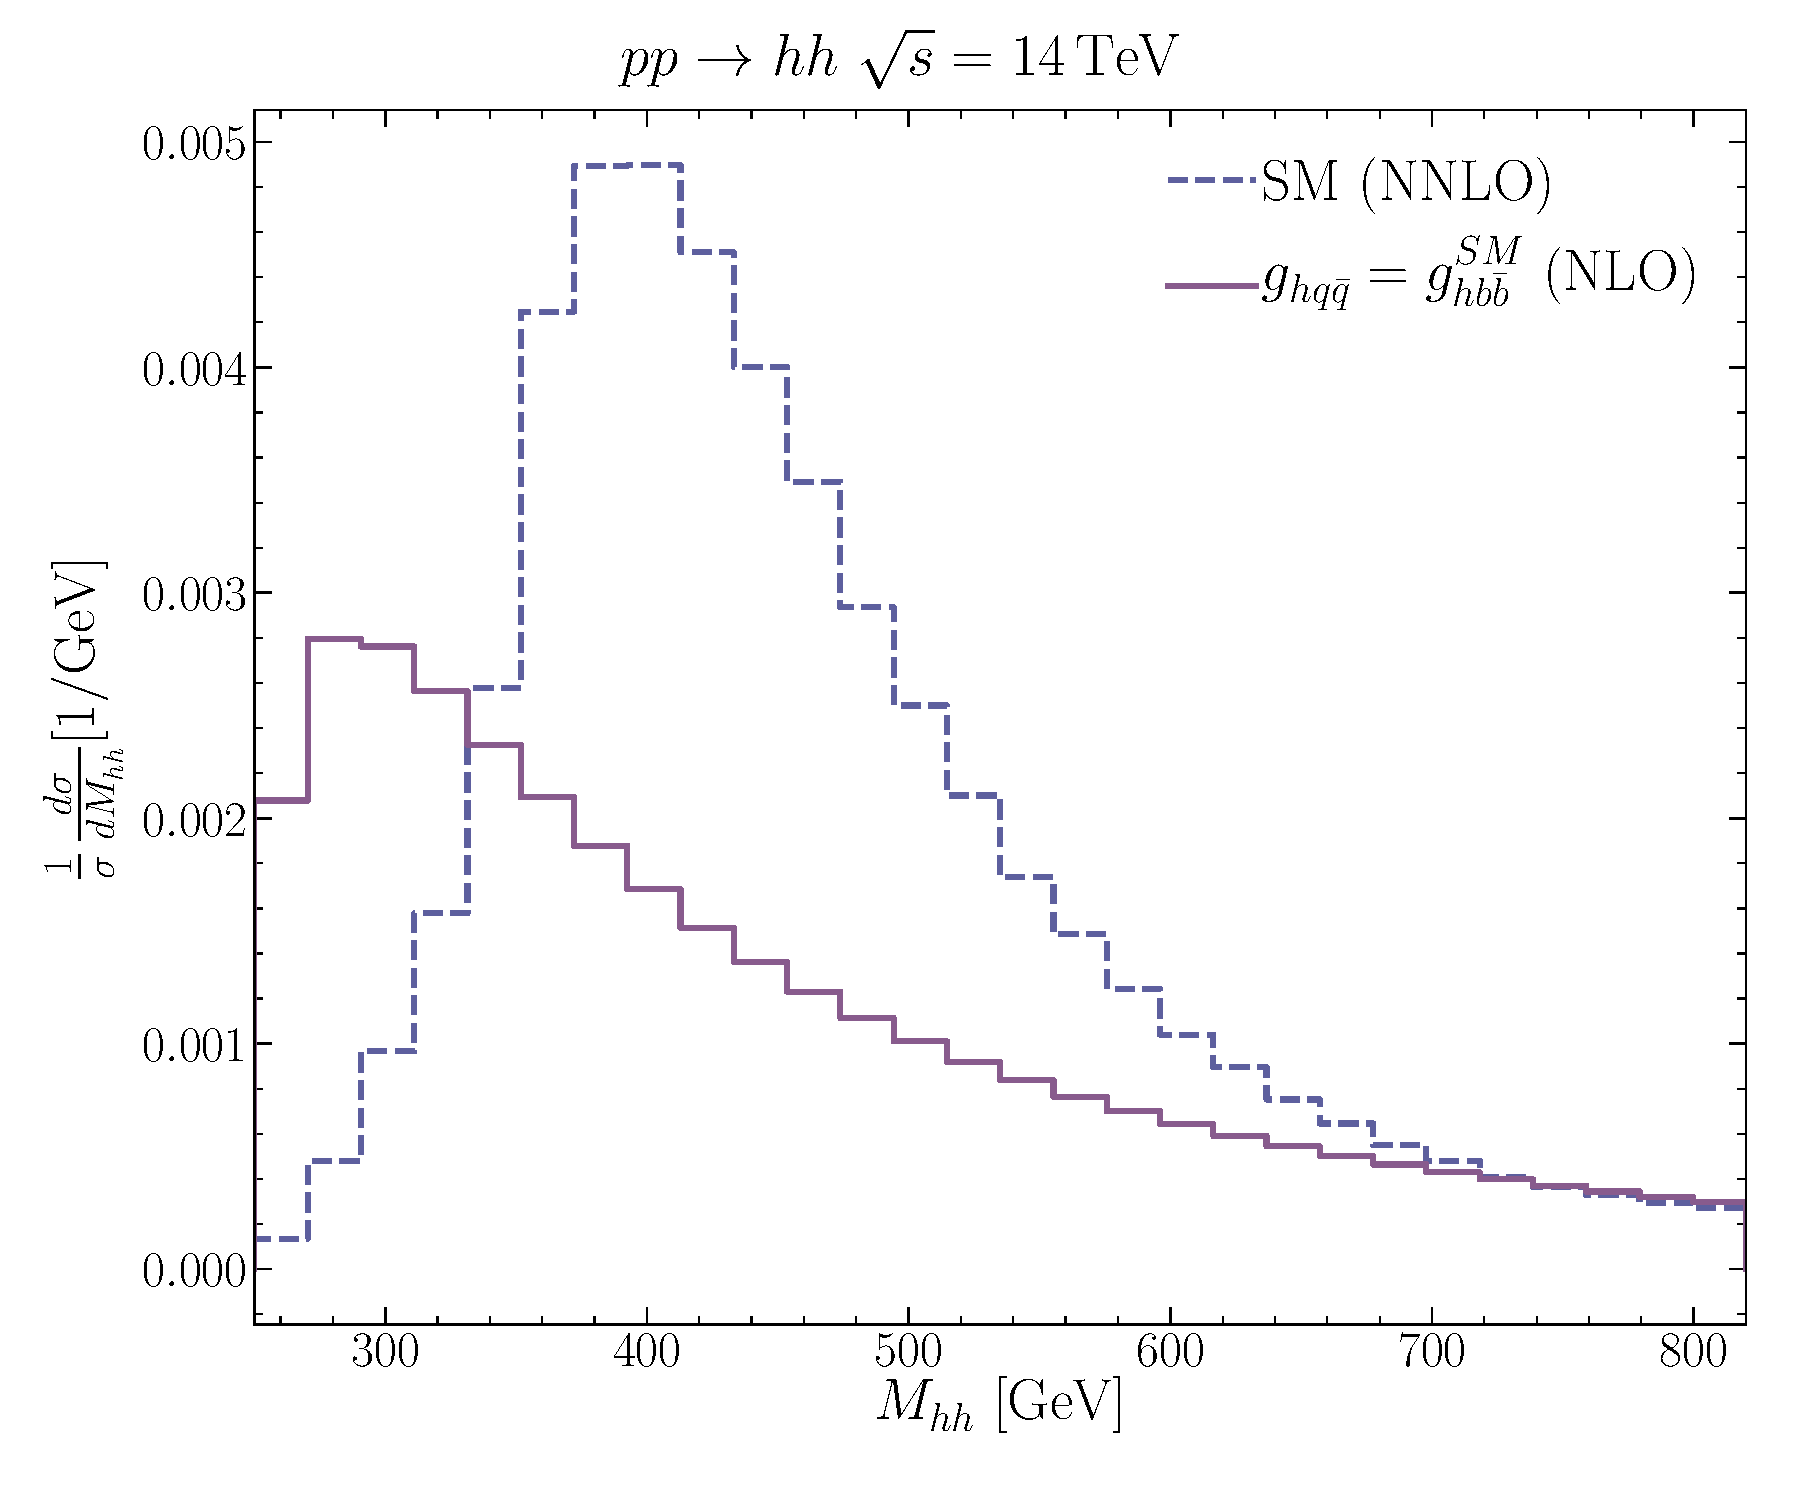
\includegraphics[width = 0.75\textwidth]{./fig/uh_shnnlo_shape.pdf}
	\caption{The qqA normalised NLO invariant mass differential cross section distribution for the benchmark point ($g_{hq \bar q} = g_{h b \bar b}^{\SM}$) (solid line) and the NNLO SM ggF cross section obtained from~\cite{Grazzini:2018bsd} (dashed line).
		}
	\label{qqA_dsigdmhh}
\end{figure}

\subsection{Higgs decays \label{sec:Hdecay}}
The light fermion decay channels will no longer be negligible for enhanced light Yukawa couplings. The decay channels $ h \to gg$, $h \to \gamma \gamma$  and $h \to Z \gamma$ containing fermion loops will get modified, but similarly to the production, the modification is ~$\sim 2\,\kappa_q\,(m_q^2/m_h^2) \,\ln^2(m_q/m_h)$. Thus, the main effect on the Higgs boson branching ratios and width is the `opening' of the new light fermion channels. \\ In order to compute the Higgs partial widths and branching ratios (BR) at higher orders in QCD, we have modified the FORTRAN programme \texttt{HDECAY}~\cite{Djouadi:1997yw,Djouadi:2018xqq} to include the light fermion decay channels and loops in the above-mentioned decays. In the SM, light fermion BRs are of order $\mathcal{O}(10^{-4})$ for $ h \to c \bar{c} $,  $\mathcal{O}(10^{-6})$ for $ h \to s \bar{s} $  and  $<\mathcal{O}(10^{-9})$ for the first generation quarks \cite{deFlorian:2016spz}. In our benchmark point ($g_{hq \bar q} = g_{h b \bar b}^{\SM}$) these would increase to $ \sim 18 \%$. Correspondingly, the BRs for  $ h \to b \bar b/VV/\tau^+\tau^-$ decrease due to the increased Higgs width in the model.
\par
In fig.~\ref{brs} we show the BRs, denoted by $\mathcal{B}$ in the following,  of the Higgs boson pair with the best prospects for discovering Higgs pair production, $hh\to b\bar{b}b\bar{b}$, $hh\to b\bar{b}\gamma\gamma$ and $hh\to b\bar{b}\tau^+\tau^-$ \cite{Aad:2019uzh}, and in addition we show for later purpose also  $hh\to c\bar{c}\gamma\gamma$. Once we increase the light quark Yukawa couplings (shown for the different quarks by the different coloured lines) the BRs to $b\bar{b}b\bar{b}$, $b\bar{b}\gamma\gamma$ and $b\bar{b}\tau^+\tau^-$ decrease due to the increased Higgs width. Instead the $\mathcal{B}(hh\to c\bar{c}\gamma\gamma)$ first increases with increasing $\kappa_c$, but starts decreasing after reaching a maximum around $\kappa_c\approx 8$, where the $\mathcal{B}(h\to c\bar{c})$ asymptotically reaches 1 while the $\mathcal{B}(h\to \gamma \gamma)$ continues decreasing.

\begin{figure}[!t]
	\centering
	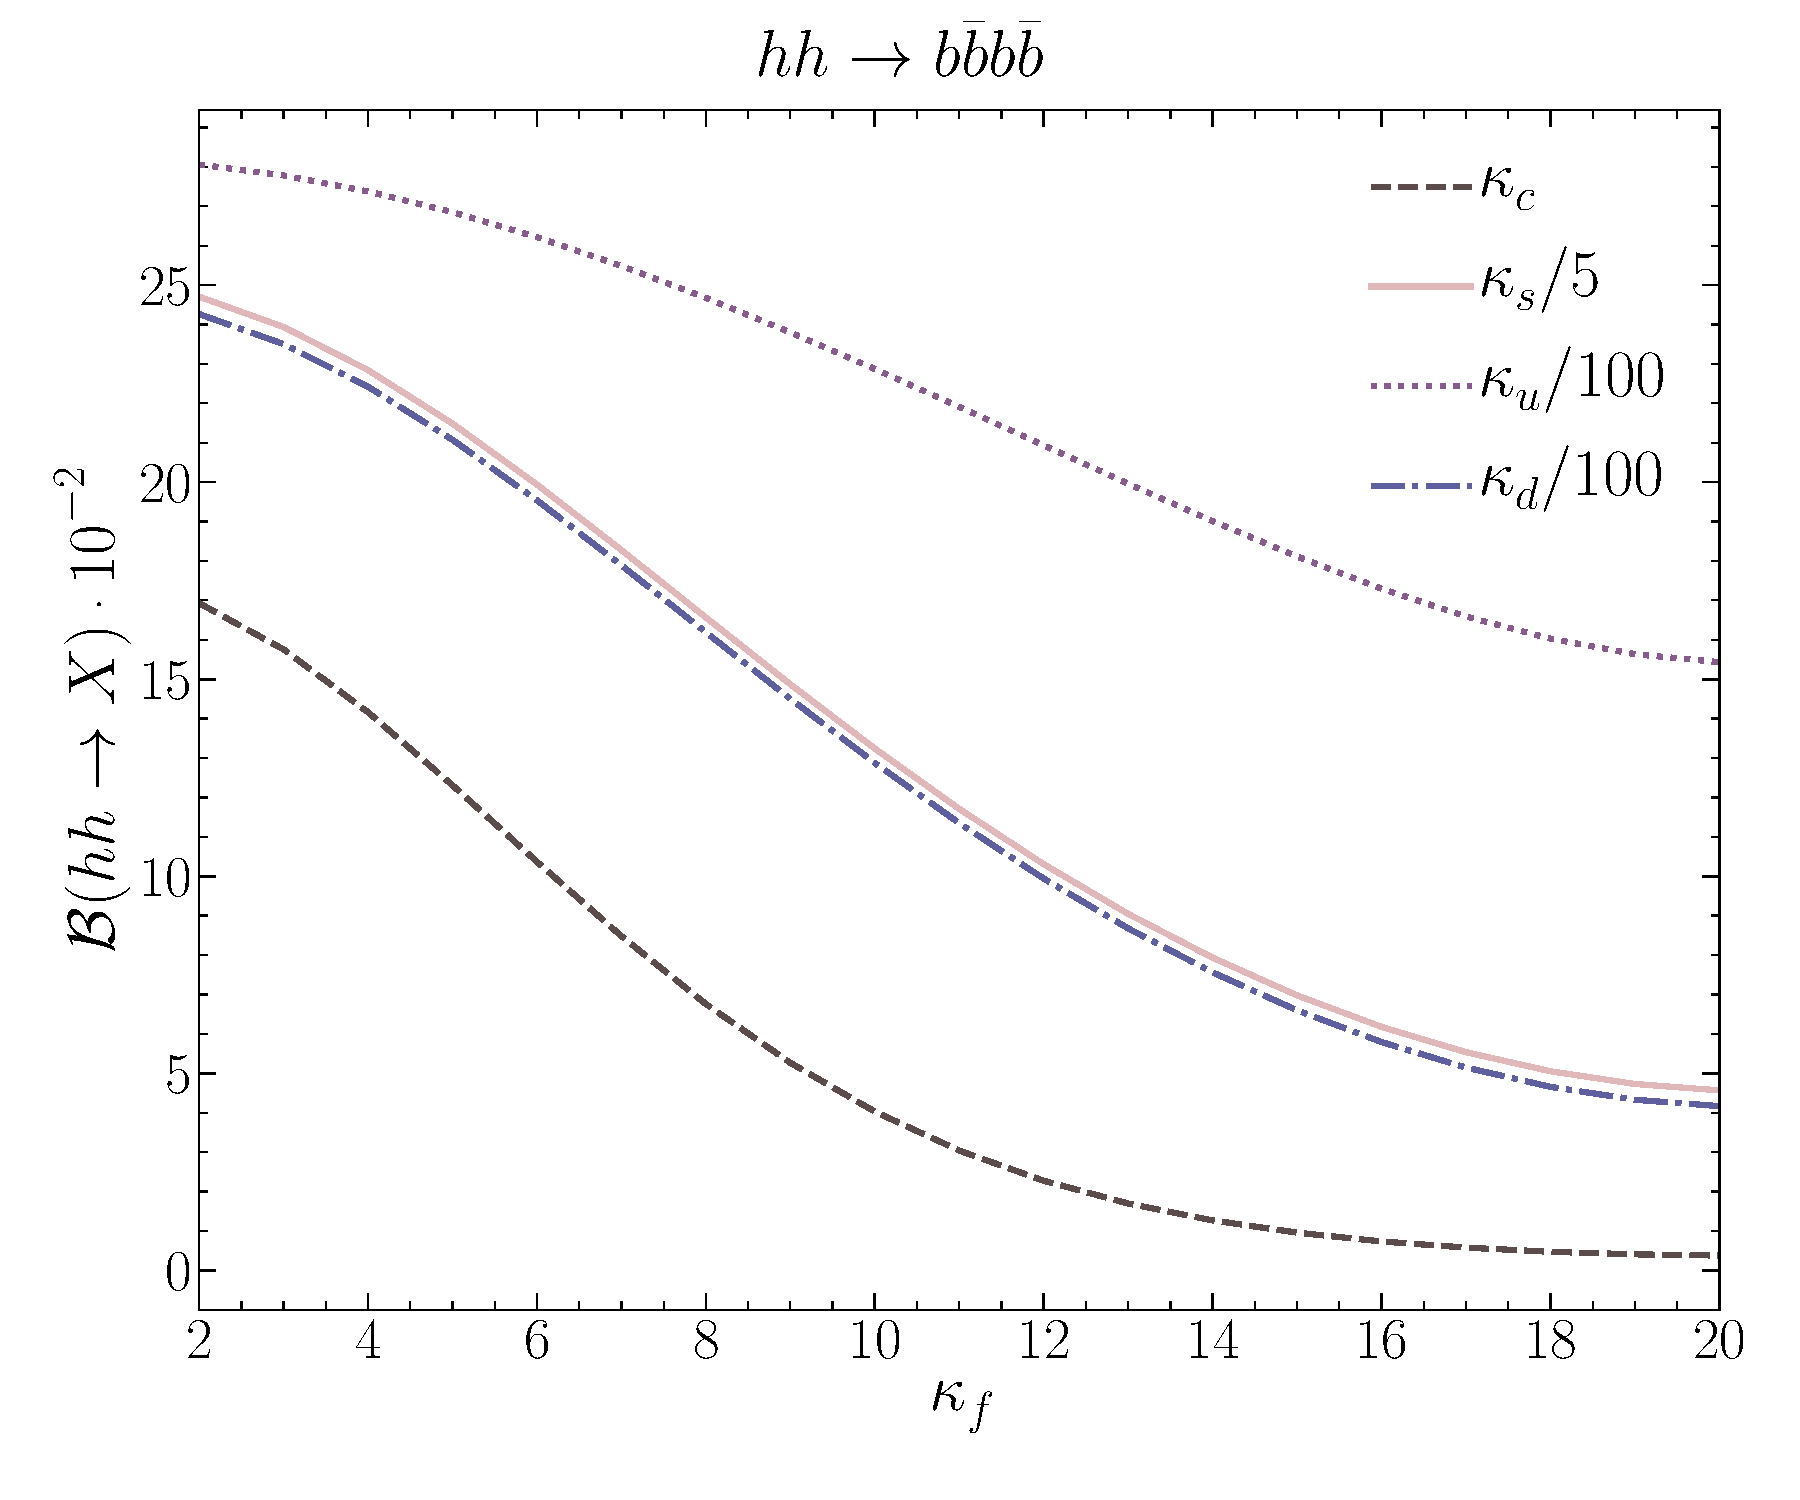
\includegraphics[width = 0.49\textwidth]{./fig/br_bbbb_kf}
	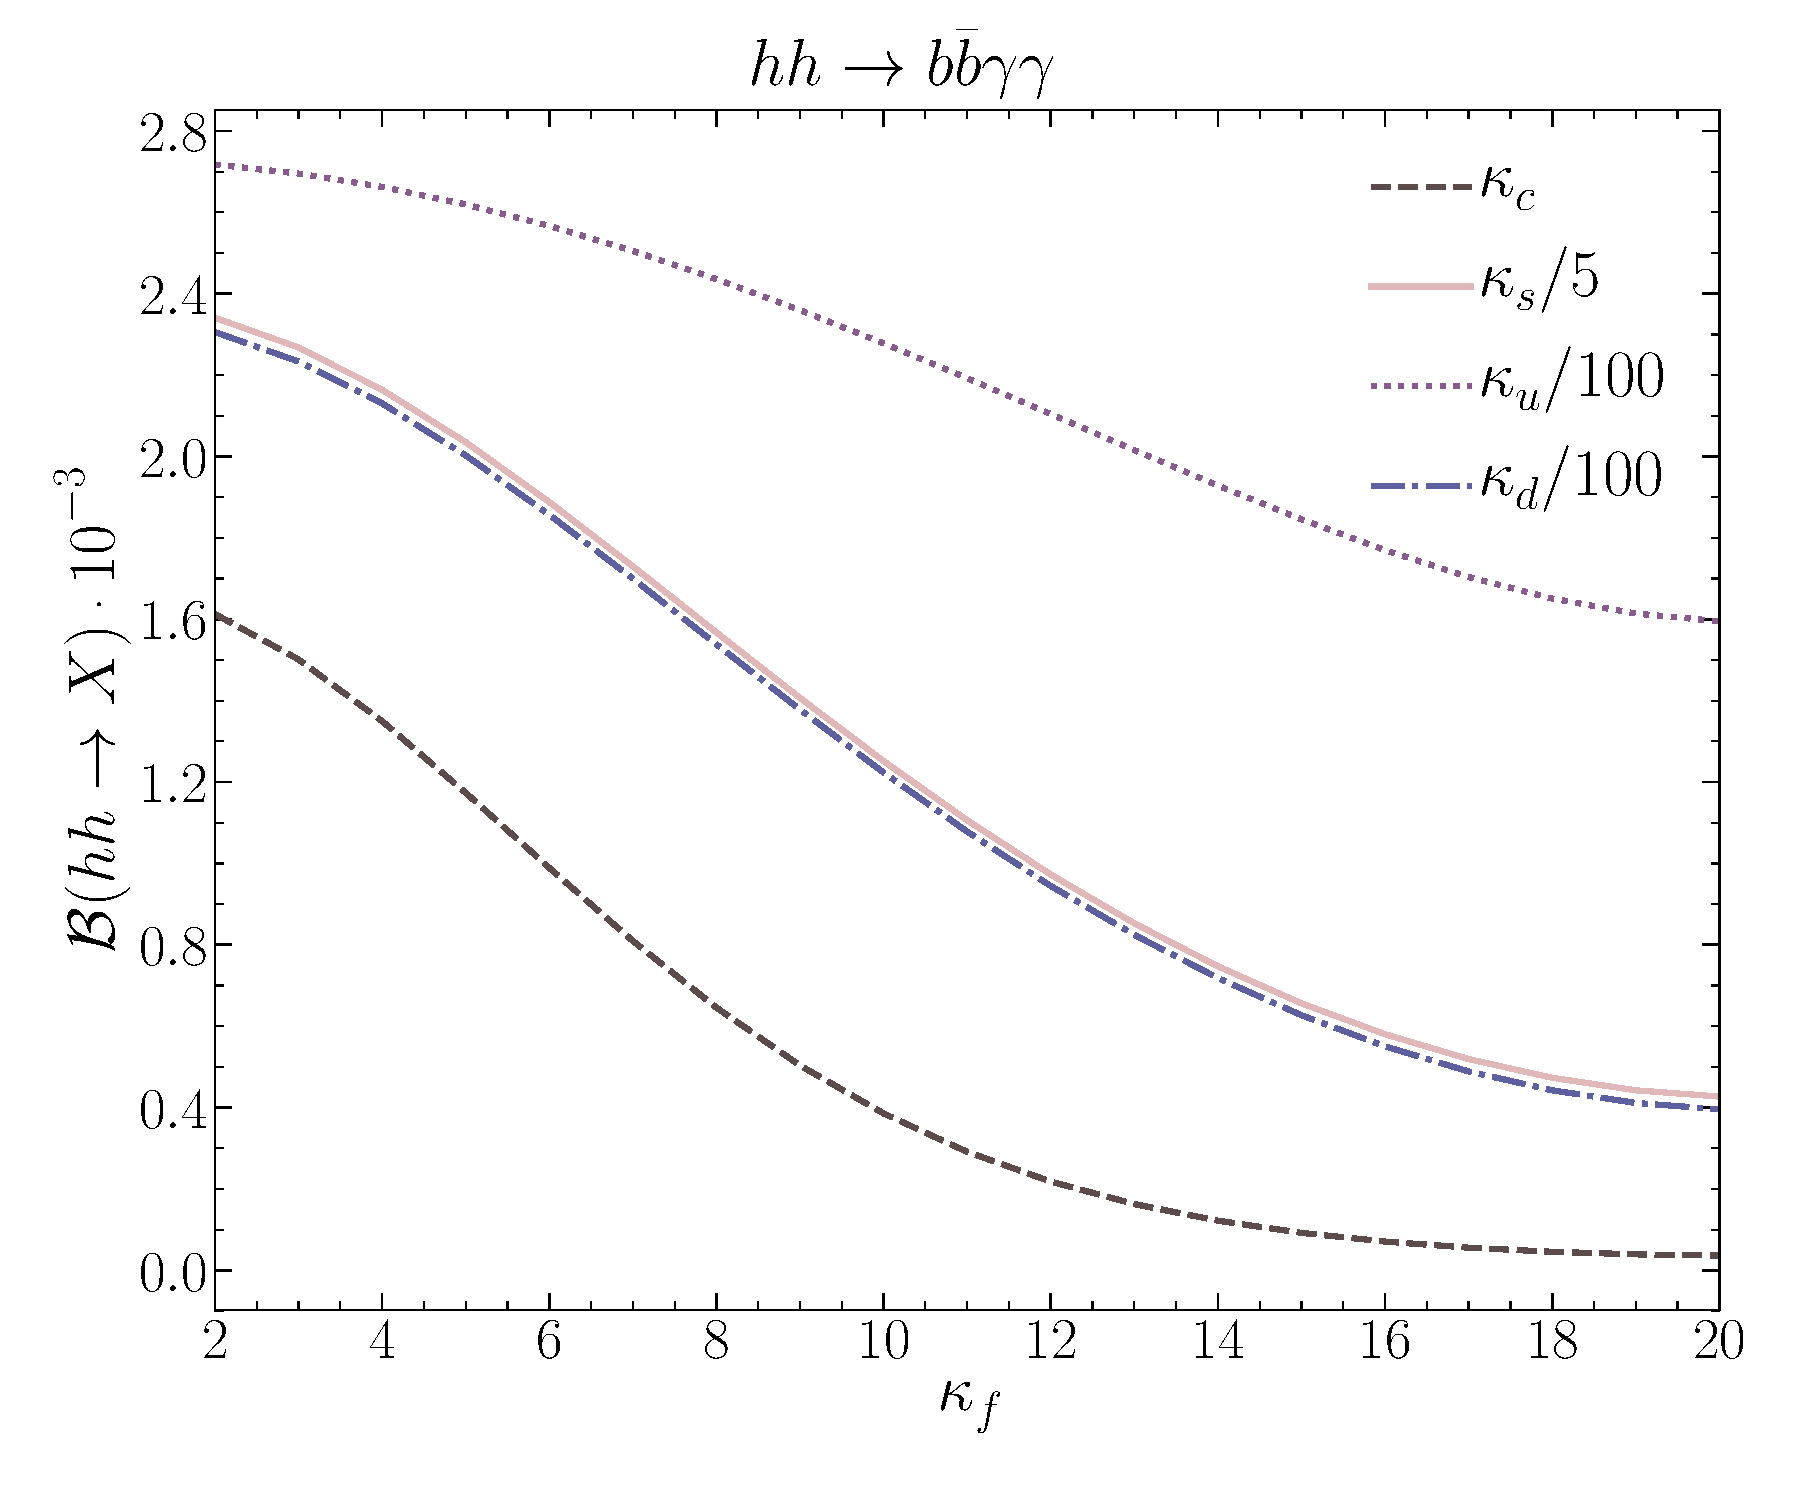
\includegraphics[width = 0.49\textwidth]{./fig/br_bbgg_kf}
	\\
	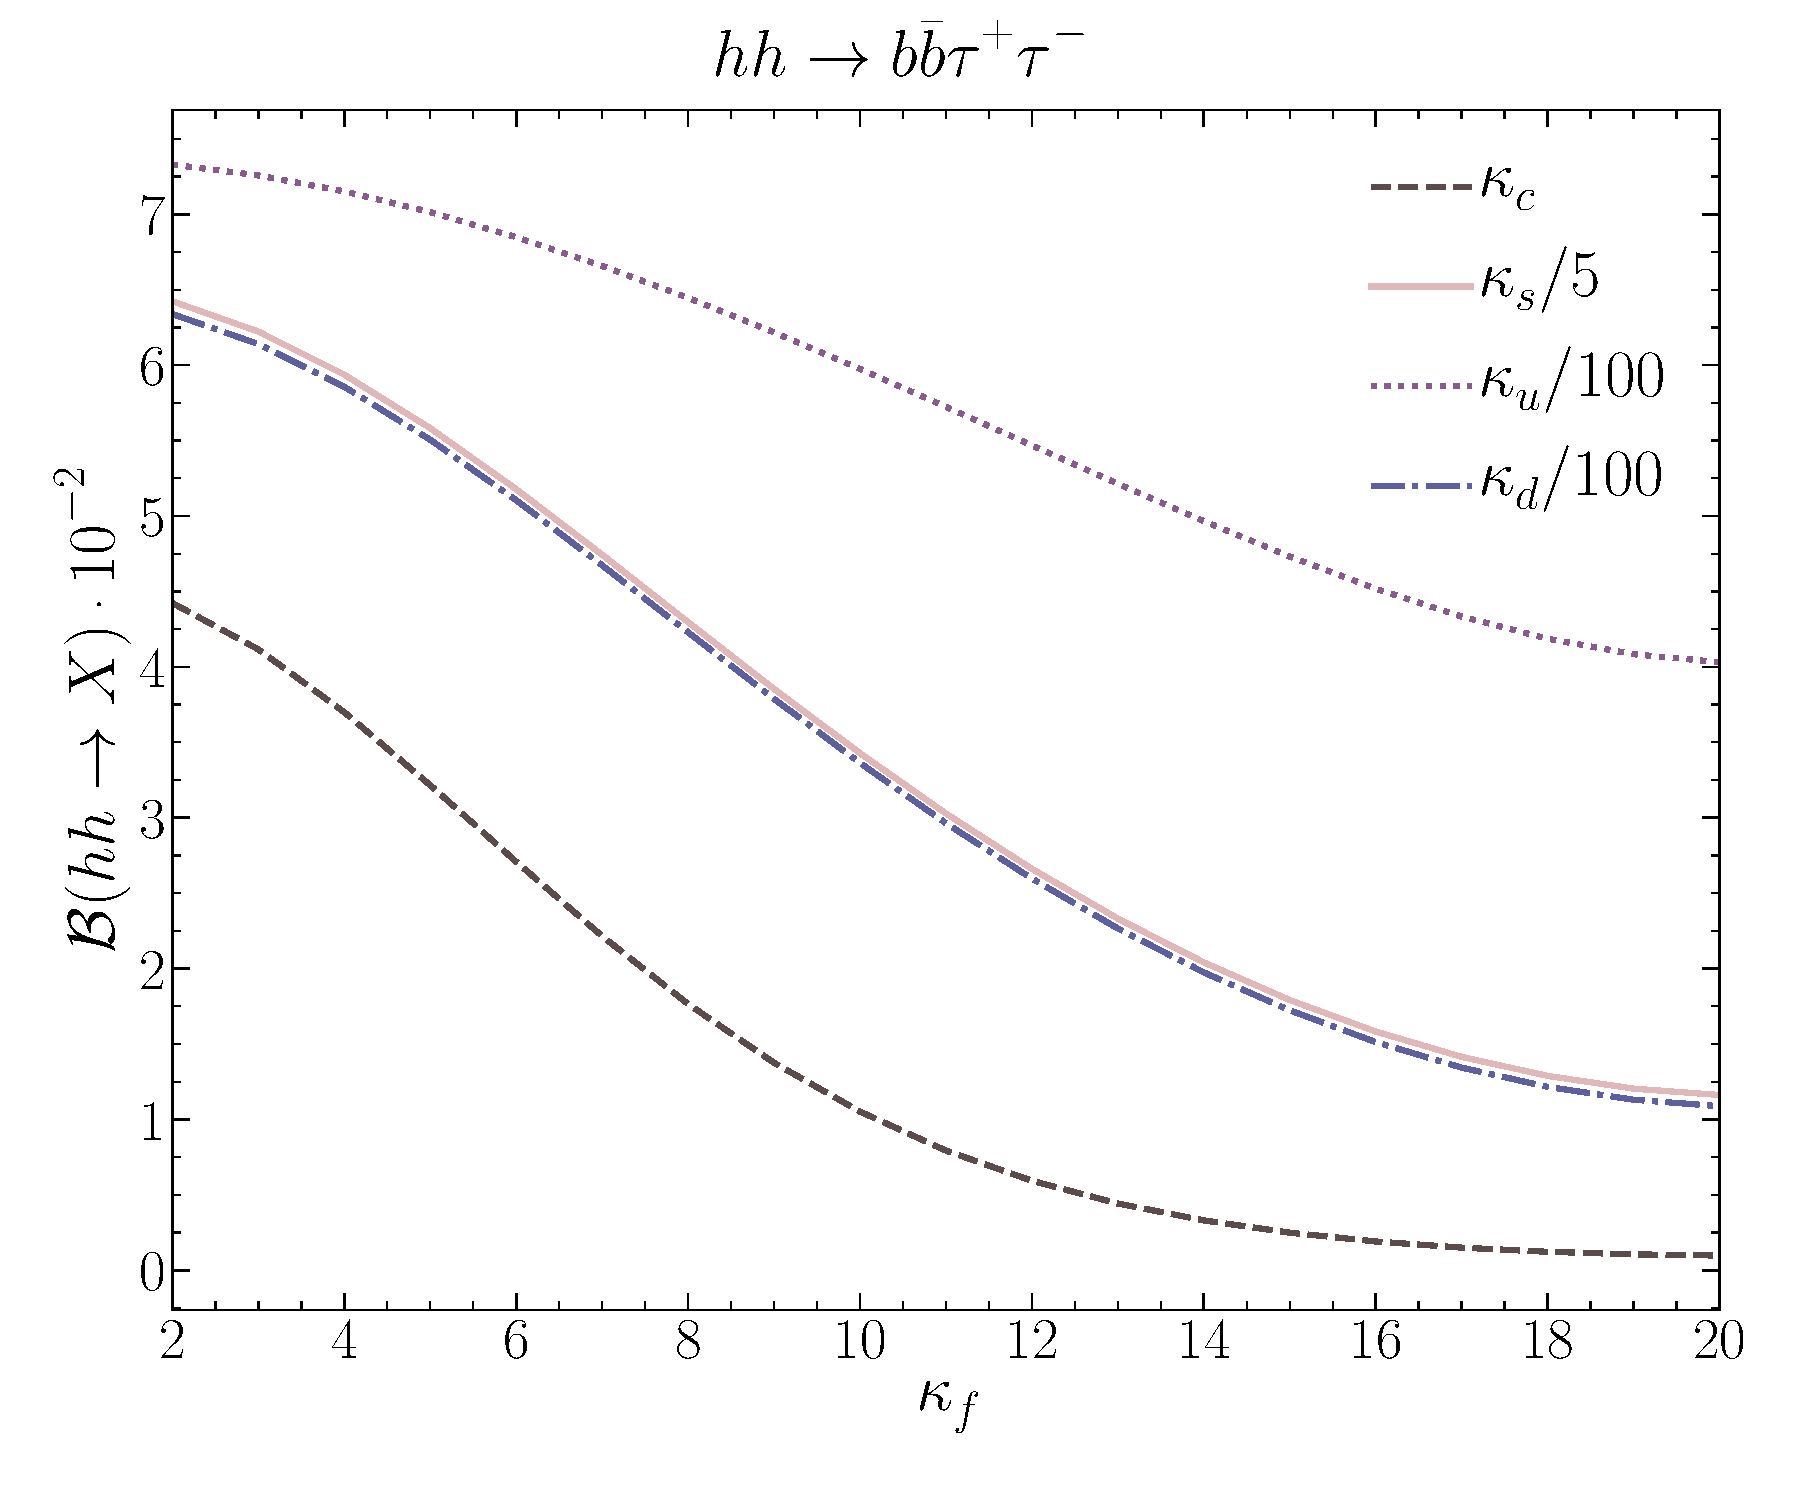
\includegraphics[width = 0.49\textwidth]{./fig/br_bbll_kf}
	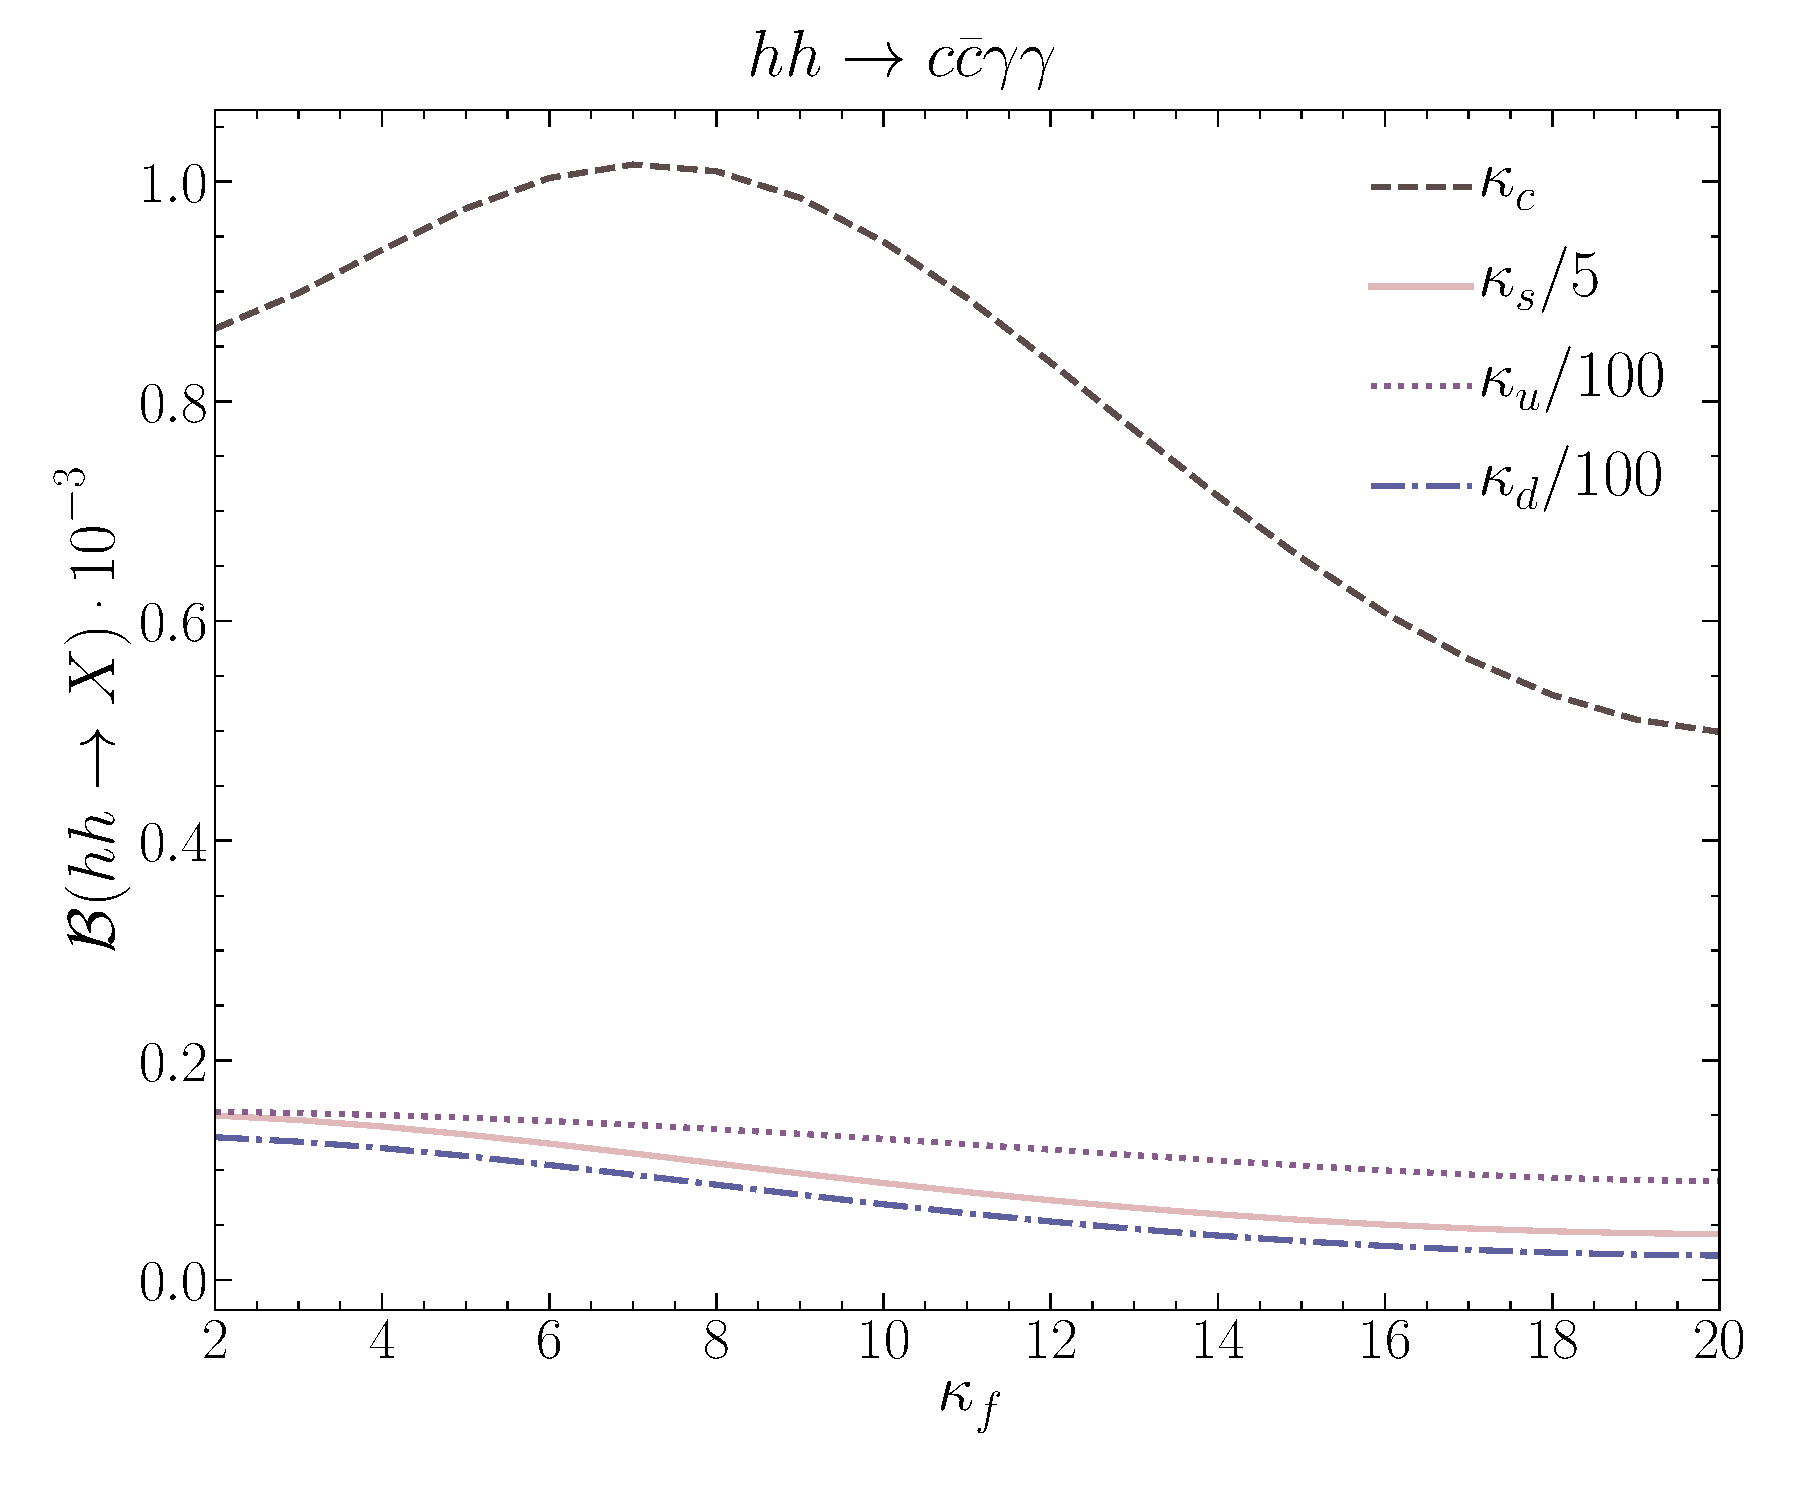
\includegraphics[width = 0.49\textwidth]{./fig/br_ccgg_kf}
	\caption{Different Higgs pair final states BRs including state-of-the-art QCD corrections as functions of the coupling modification factors $\kappa_f$. \textit{Top left}: $ hh \to b \bar b b \bar b$. \textit{Top right}: $ hh \to b \bar b \gamma \gamma$. \textit{Bottom left}: $ hh \to b \bar b \tau^+ \tau^-$. \textit{Bottom right}: $ hh \to c \bar c \gamma \gamma$. }
	\label{brs}
\end{figure}
In fig.~\ref{kcks_mu_contors} we show the signal strength modifier defined  here as\\

\begin{equation}
	\mu_i : = \frac{\sigma \, {\cal B}_i } {\sigma^{\SM} \, {\cal B}_i^{\SM}}\quad \quad (i=b,c),
\end{equation}
for final states with bottom (left hand side) and charm quarks (right hand side) for first generation (plots in the upper row) and second generation (plots in the lower row) modified Yukawa couplings. For the first generation, we obtain enhancement of both of the signal strengths $\mu_c$ and $\mu_b$, as seen  plots in the top of fig.~\ref{kcks_mu_contors}. The  second generation  signal strength is instead reduced with respect to the SM for the channels with bottom quarks in the final state $\mu_b : = \sigma \, {\cal B}_b/ \sigma ^{\SM}\, {\cal B}_b^{\SM}$ when scaling the charm and strange Yukawa couplings, as seen in the lower left plot of fig.~\ref{kcks_mu_contors}. Nevertheless, when considering channels with charm quarks in the final state the signal strength $\mu_c : = \sigma \, {\cal B}_c /\sigma^{\SM} \, {\cal B}_c^{\SM} $ is enhanced due to both enhancements from the cross section and BRs.
\begin{figure}[!t]
	\centering
	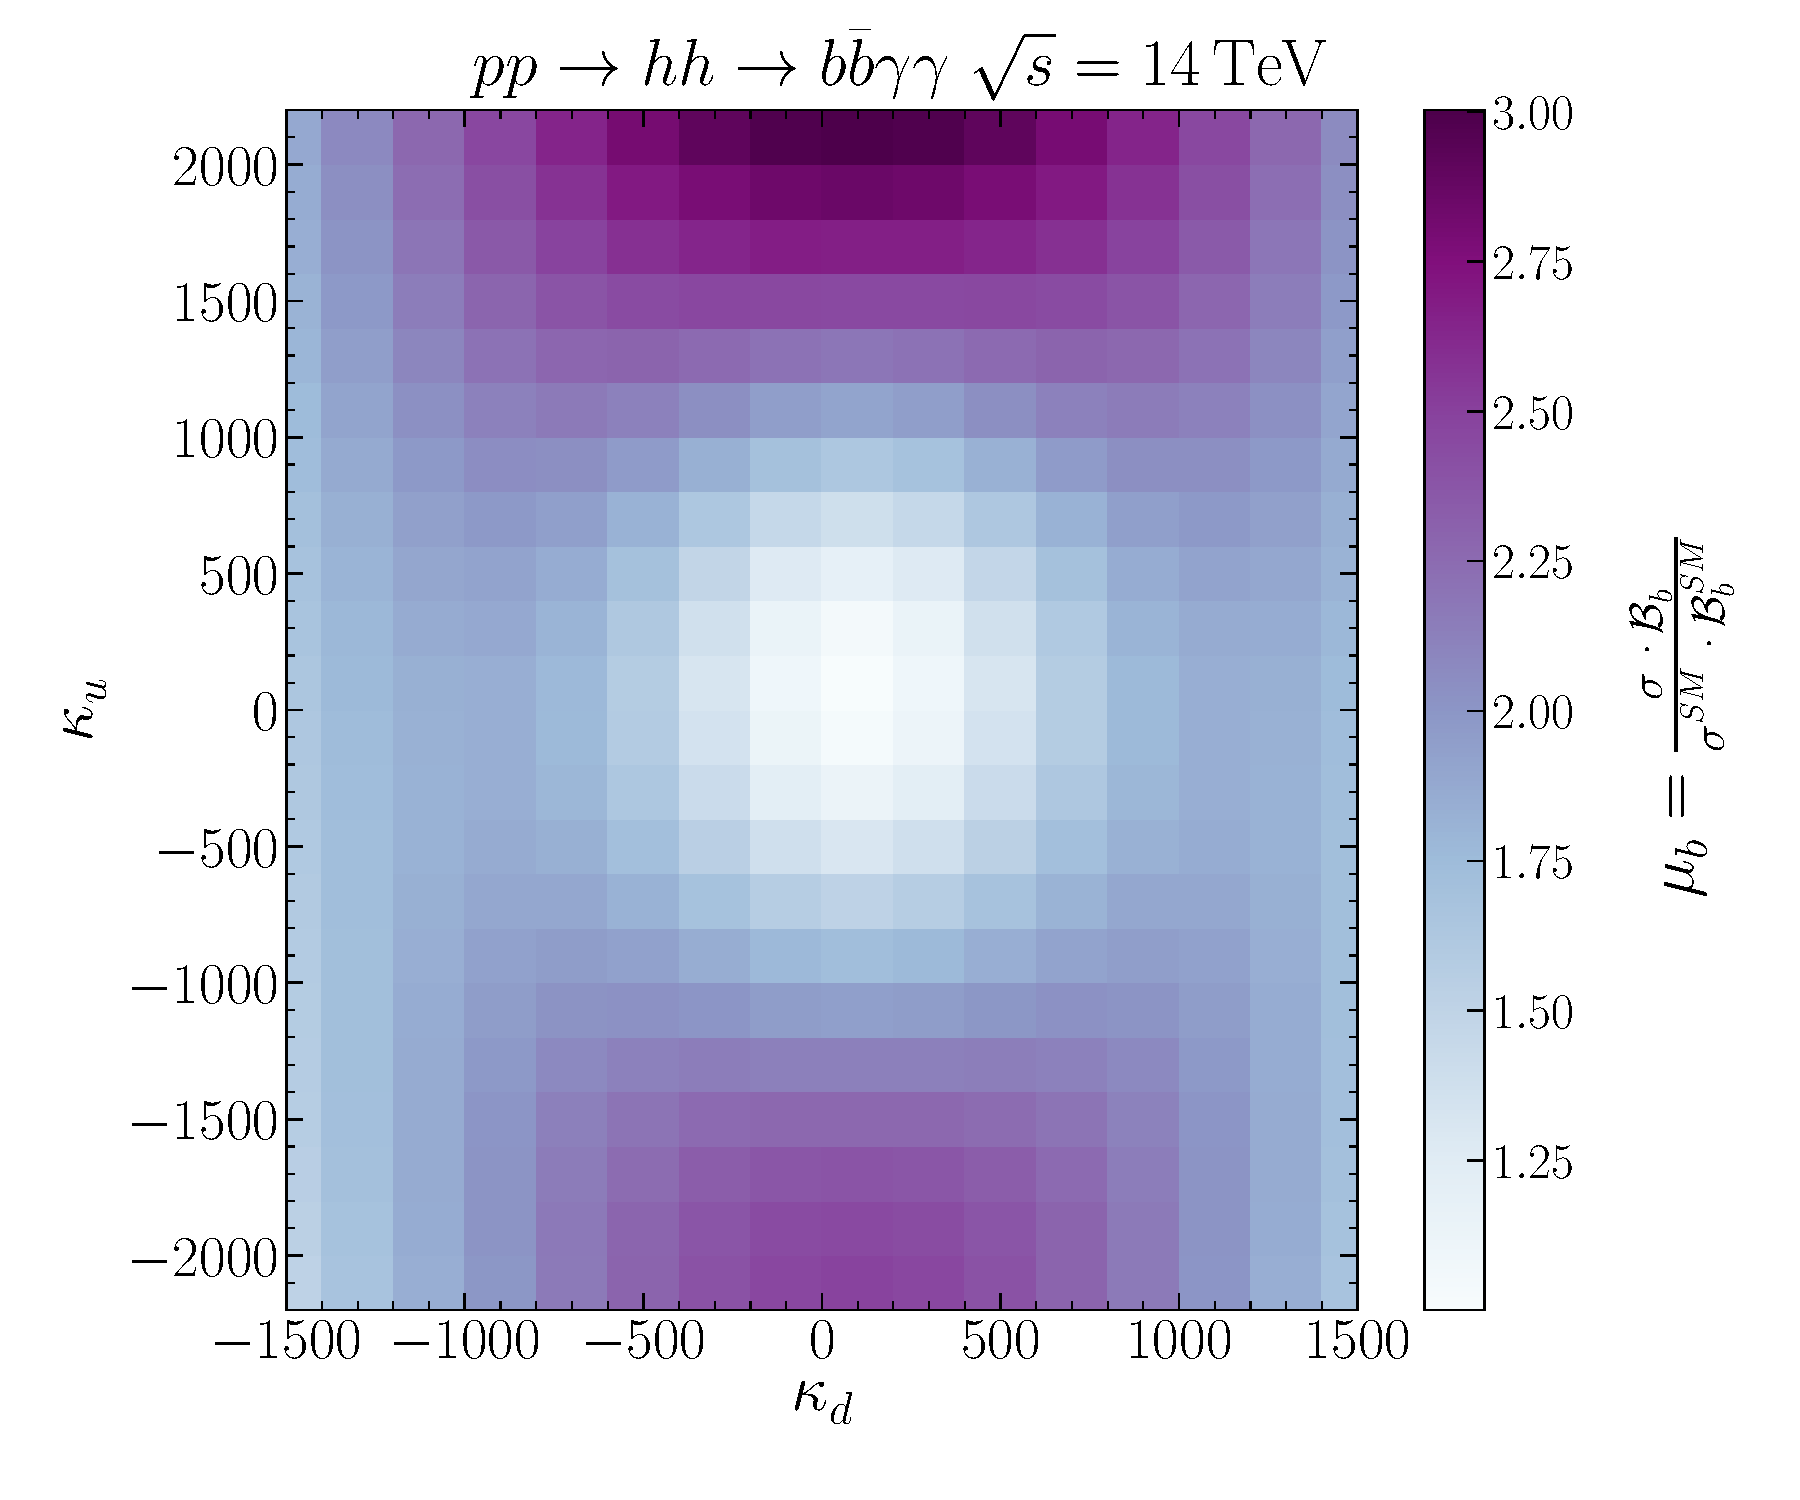
\includegraphics[width = 0.49\textwidth]{./fig/mub_fit_kdku.pdf}
	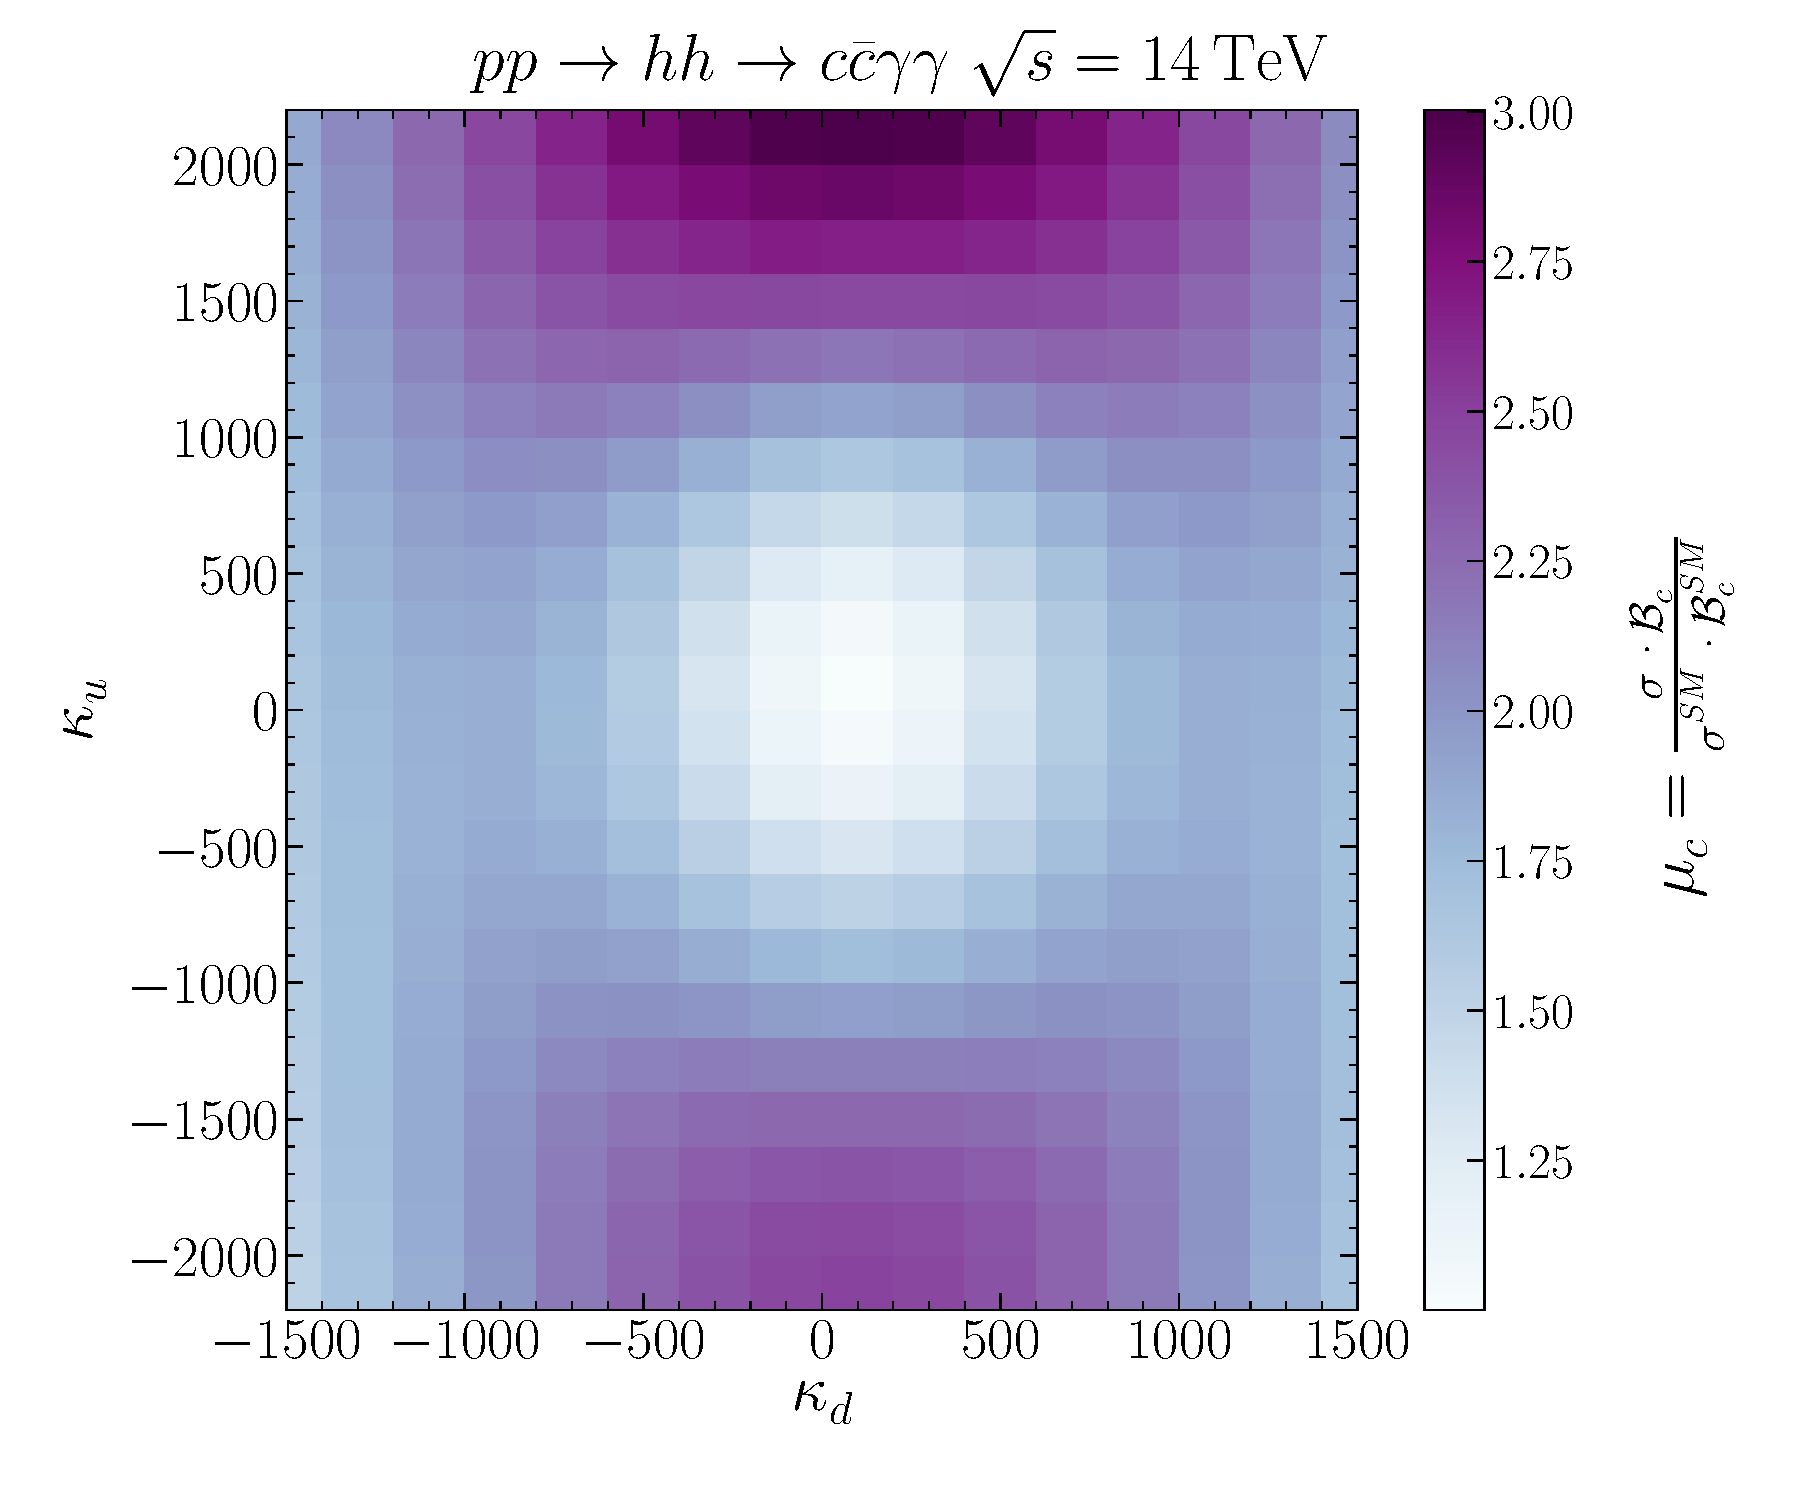
\includegraphics[width = 0.49\textwidth]{./fig/muc_fit_kdku}
	\\
	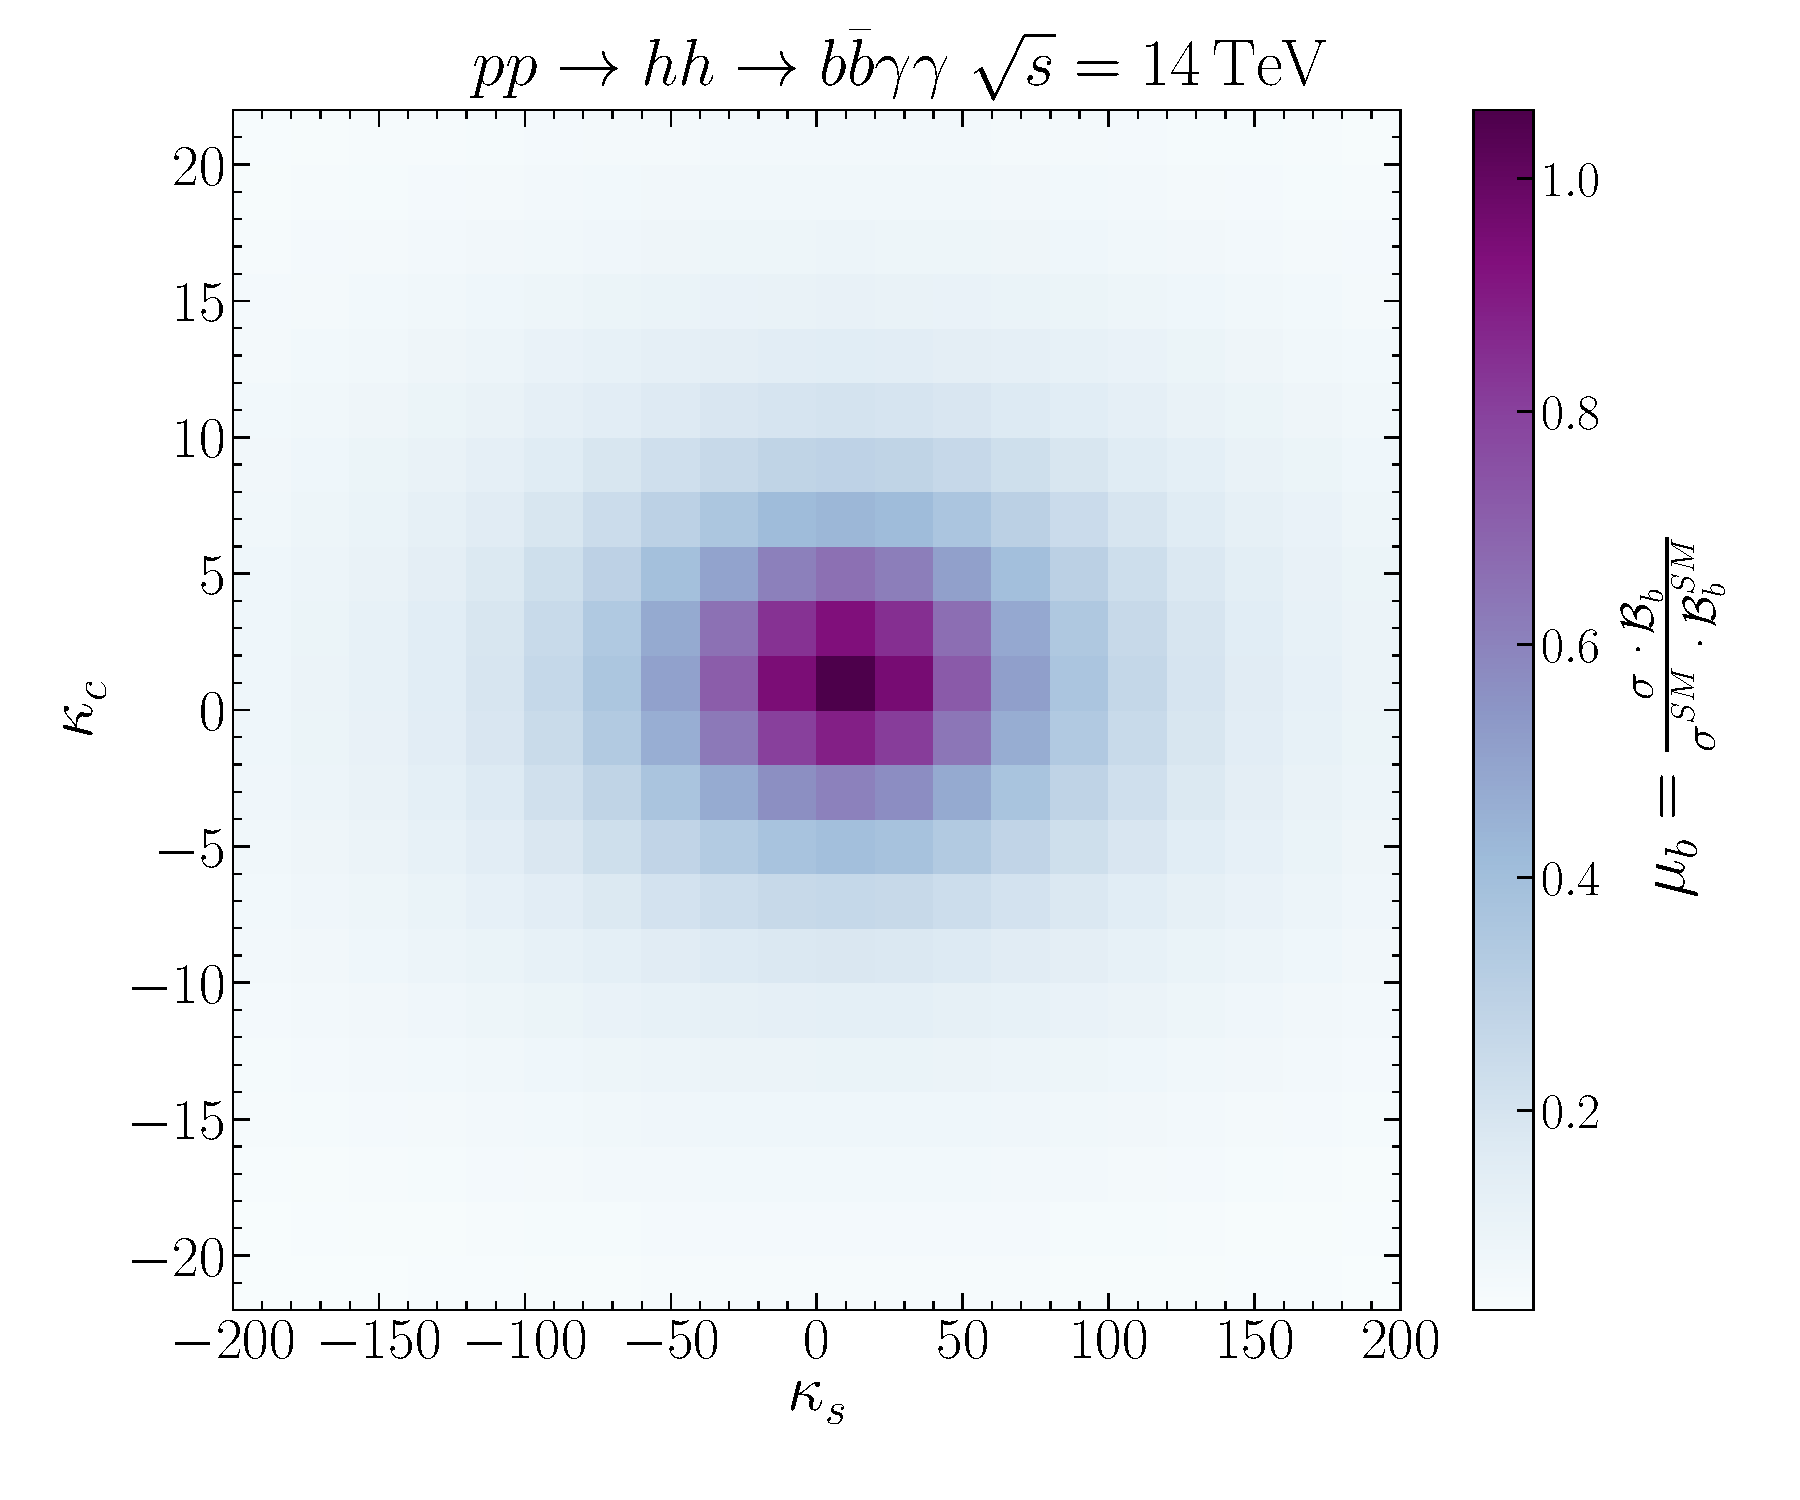
\includegraphics[width = 0.49\textwidth]{./fig/mub_fit_kskc}
	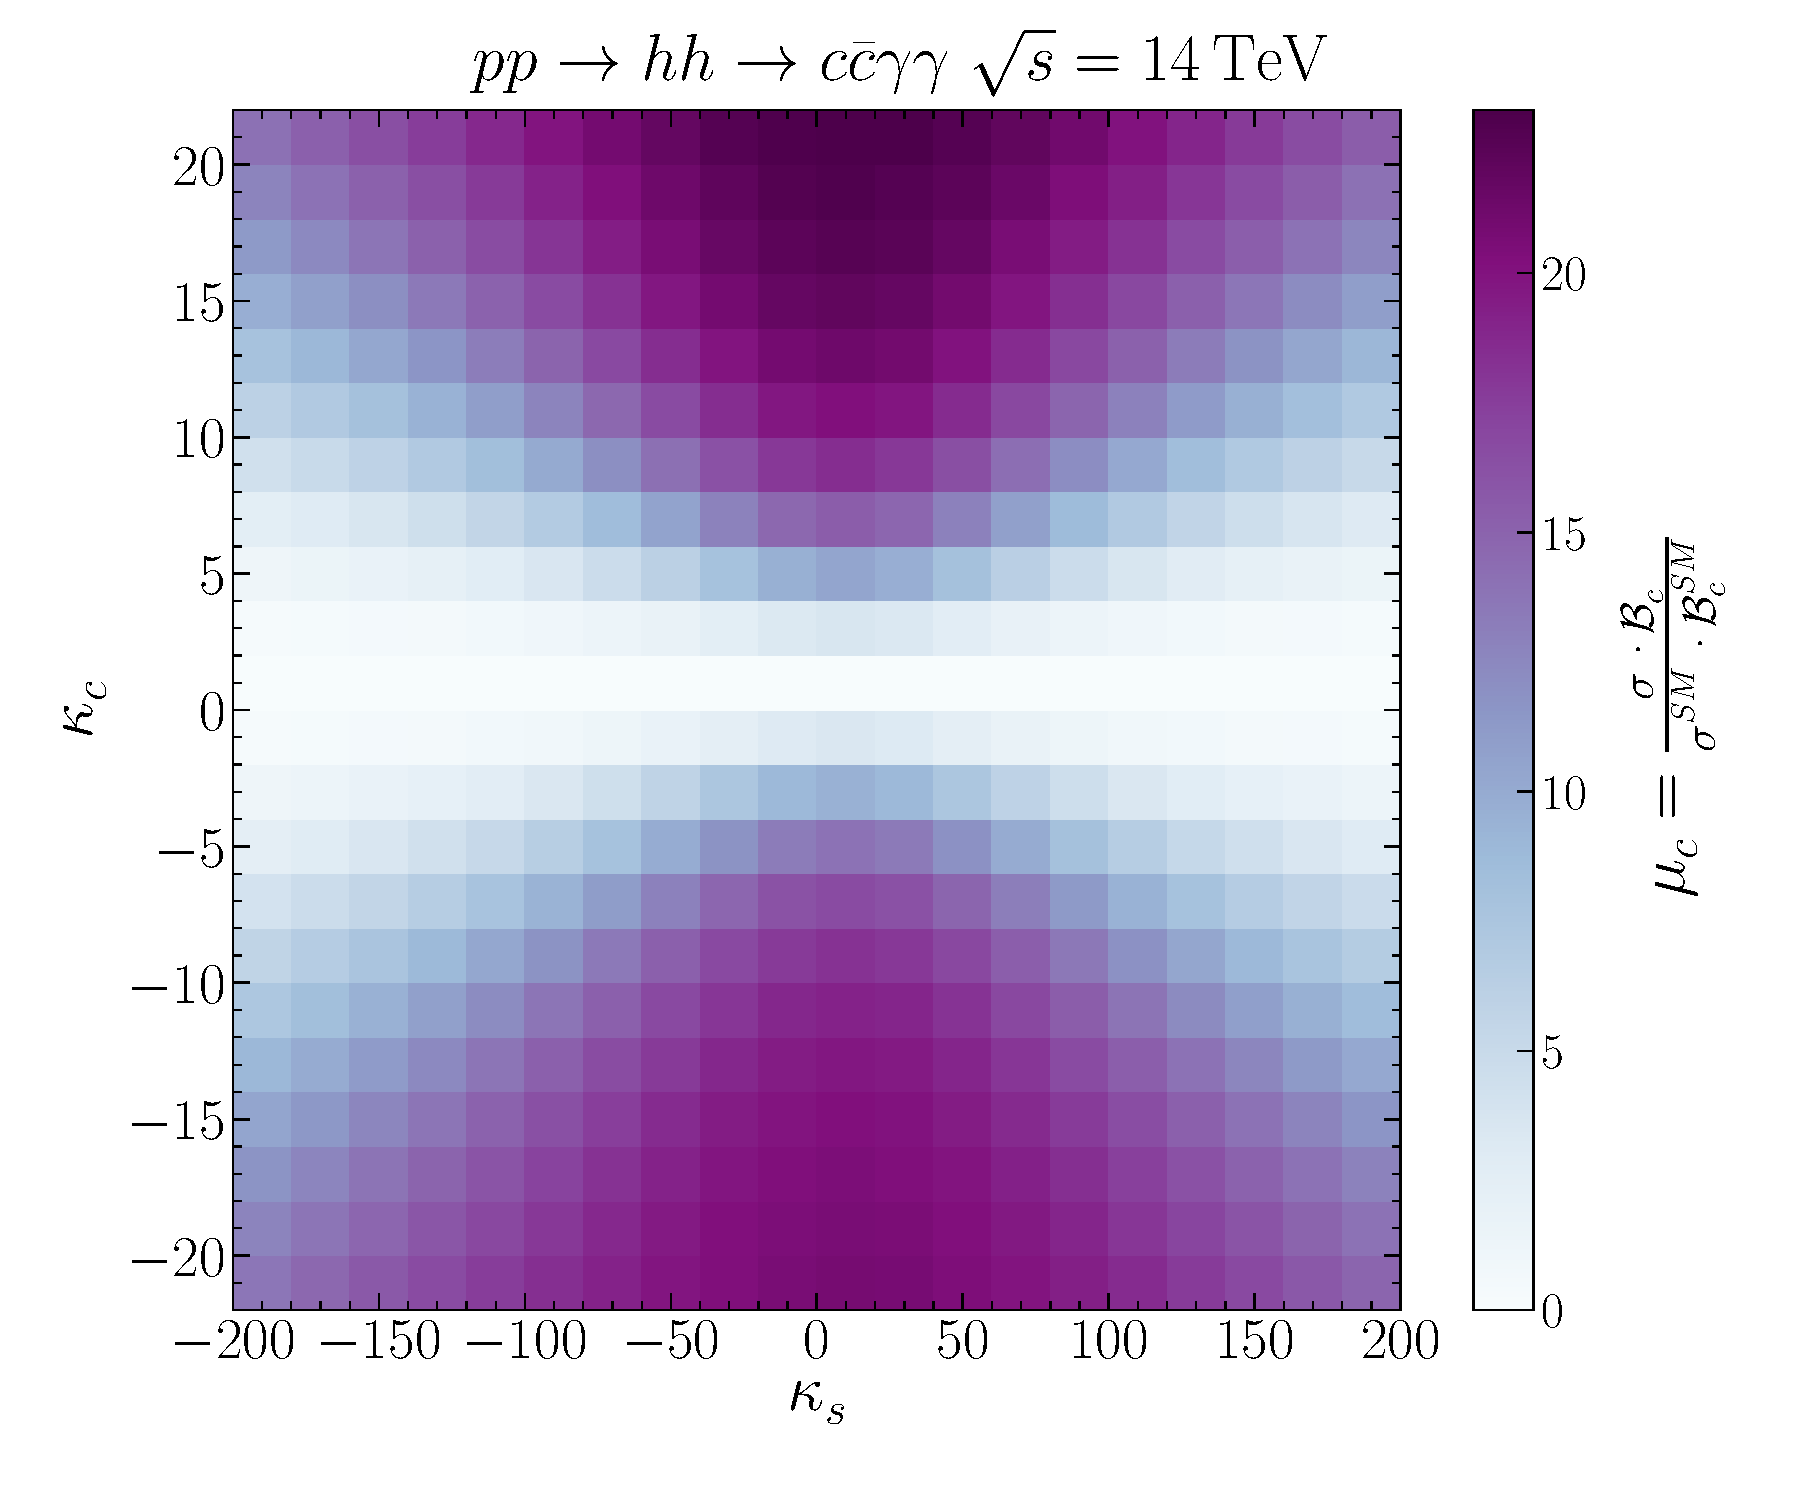
\includegraphics[width = 0.49\textwidth]{./fig/muc_fit_kskc}
	\caption{Signal strength modifier $\mu = \sigma \,{\cal B}(hh \to X) / (\sigma^{SM} \,{\cal B}^{SM}(hh \to X) )$  fits for bottom quark (left plots) and charm quark (right plots)  final states for  first~(upper row) and second~(lower row) generations quark Yukawa modifications.}
	\label{kcks_mu_contors}
\end{figure}
The increased cross section in the presence of enhanced light quark Yukawa couplings has to compete with the decreased BRs for the standard search channels for di-Higgs production.
We shall notice however, that while the increase of the cross section comes mainly from the $q\bar{q}hh$ vertex diagram, the decrease of the BRs stems from the increased width which would be in good approximation (for flavour-diagonal couplings)
\begin{equation}
	\Gamma_H \approx \Gamma_{\text{SM}}+\sum_{q=c,s,u,d}\frac{g_{h \bar{q}_i q_i}^2}{(g_{h \bar{q}_i q_i}^{\text{SM}})^2}\Gamma_{q}\,,
\end{equation}
where $\Gamma_q$ stands generically for the partial width of the Higgs boson decaying to light quarks.
In a non-linear EFT as briefly discussed in sect.~\ref{sec:EFT}, the couplings of one Higgs boson to quarks and two Higgs bosons to quarks are uncorrelated.
So an increase of the cross section for $hh$ production in the presence of modified light quark Yukawa couplings does not need to go hand in hand with a decrease of the BRs in the final states with bottom quarks (or at least the decrease could be in-proportional).

\section{Event generation for the final state $ hh \to b \bar b \gamma \gamma$ \label{sec:evnt}}
\section{Cut-based analysis \label{sec:cutbasedly}}
\section{Optimised search for Higgs pair via Interpretable machine learning \label{sec:mlanalysisly}}
\section{Fit results\label{sec:resultsly}}
%%%%%%%%%%%%%%%%%%%%%%%%%%%%%%%%%%%%%%%%%%%%%%%%%%
\section{Overview of Light Yukawa searches \label{sec:comparetoothers}}
%%%%%%%%%%%%%%%%%%%%%%%%%%%%%%%%%%%%%%%%%%%%%%%%%%
There are additional measurements of the light-quark Yukawa couplings that might become relevant at HL-LHC or FCC-hh, a careful study of which is beyond the scope of the current work. Yet we attempt to include a discussion here, so as to provide a comparison with our study and to put it into proper context, or to serve as proposal for further studies.

The channel $pp \to h +j $ has been suggested as a probe for charm Yukawa coupling~\cite{Brivio:2015fxa} with charm-tagged jet having a potential bound of $\kappa_c\sim 1$ for the HL-LHC, depending on the charm-tagging scheme. This process could be used for the first and second generations Yukawa couplings by looking at the shapes of kinematic distributions, the most important one being the $p_T$ distribution~\cite{Soreq:2016rae,Bishara:2016jga, Bonner:2016sdg}. The expected HL-LHC 95\% CL bounds are $\kappa_c \in [-0.6,3.0]$, $|\kappa_u |\lesssim 170 $ and $|\kappa_d| \lesssim 990$. The use of $h+j$ process along with other single Higgs processes have also been suggested as indirect probes for Higgs self coupling~\cite{McCullough:2013rea,Gorbahn:2016uoy,Bizon:2016wgr,Degrassi:2016wml,Maltoni:2017ims,Degrassi:2021uik}, due to the contribution of the trilinear coupling to NLO electroweak corrections to these processes. In addition, experimental fits have been carried out for the trilinear coupling from single Higgs observables~\cite{CMS:2018rig,ATLAS:2019pbo}. 

It seems that for the HL-LHC, an optimal bound for the trilinear coupling can be obtained by combing both the data from single-Higgs process as well as Higgs pair production~\cite{DiVita:2017eyz}, with 68\% CL bound on $\kappa_\lambda \in[0.1,2.3]$, compared to the expected bound of $\kappa_\lambda \in [0.0,2.5] \cup [4.9,7.4]$ coming from using di-Higgs measurements alone. Moreover, single Higgs processes, namely $Zh$ and $ W^\pm h$ production, could also be useful in probing charm-Yukawa coupling using a mixture of $b$- and $c$-tagging schemes leveraging the mistagging probability of $c$-jets as $b$-jets in $b$-tagging working points, and vice-versa, in order to break the degeneracy in the signal strength~\cite{Perez:2015lra}. The use of this technique could probe $\kappa_c \sim 1$ in the FCC-hh. Of course, for the charm-Yukawa coupling, the constraints are set to improve significantly, as there has been recent direct observation of $h\to c \bar c$~\cite{ATLAS-CONF-2021-021}. Therefore, from here on, we will mainly concentrate  on the process with more potential for constraining Yukawa couplings of the first generation quarks. 

Rare Higgs decays to mesons, $h \to M +V ,\, \, M = \Upsilon, J/\Psi, \phi\dots$, were also suggested as a probe for light-quark Yukawa couplings~\cite{Bodwin:2013gca,Kagan:2014ila,Konig:2015qat}, and there have been experimental searches for these decays~\cite{ATLAS-CONF-2021-021,CMS:2018gcm} with bounds on the branching ratios, $\mathcal{B} (h \to X, \gamma, \,\,\, X =\Upsilon, J/\Psi,  ) \sim 10^{-4} - 10^{-6}$ at 95\% CL. It was shown in Ref.~\cite{Yu:2017vul}, that the charge asymmetry of the process $pp \to h W^+$ vs $ pp \to h W^-$ can be used as a probe for light-quark Yukawa couplings as well as to break the degeneracy amongst quark flavours. Moreover, the rare process $ pp \to h \gamma$ is also a possible way to distinguish between enhancements of the up- and down-Yukawa couplings~\cite{Aguilar-Saavedra:2020rgo} where the authors have estimated the bounds on the up-Yukawa coupling of $\kappa_u\sim 2000$ at the HL-LHC. Despite some processes appearing more sensitive than others, one should think of these processes as complementary to each other. 

\begin{figure}[t!]
	%	\centering
	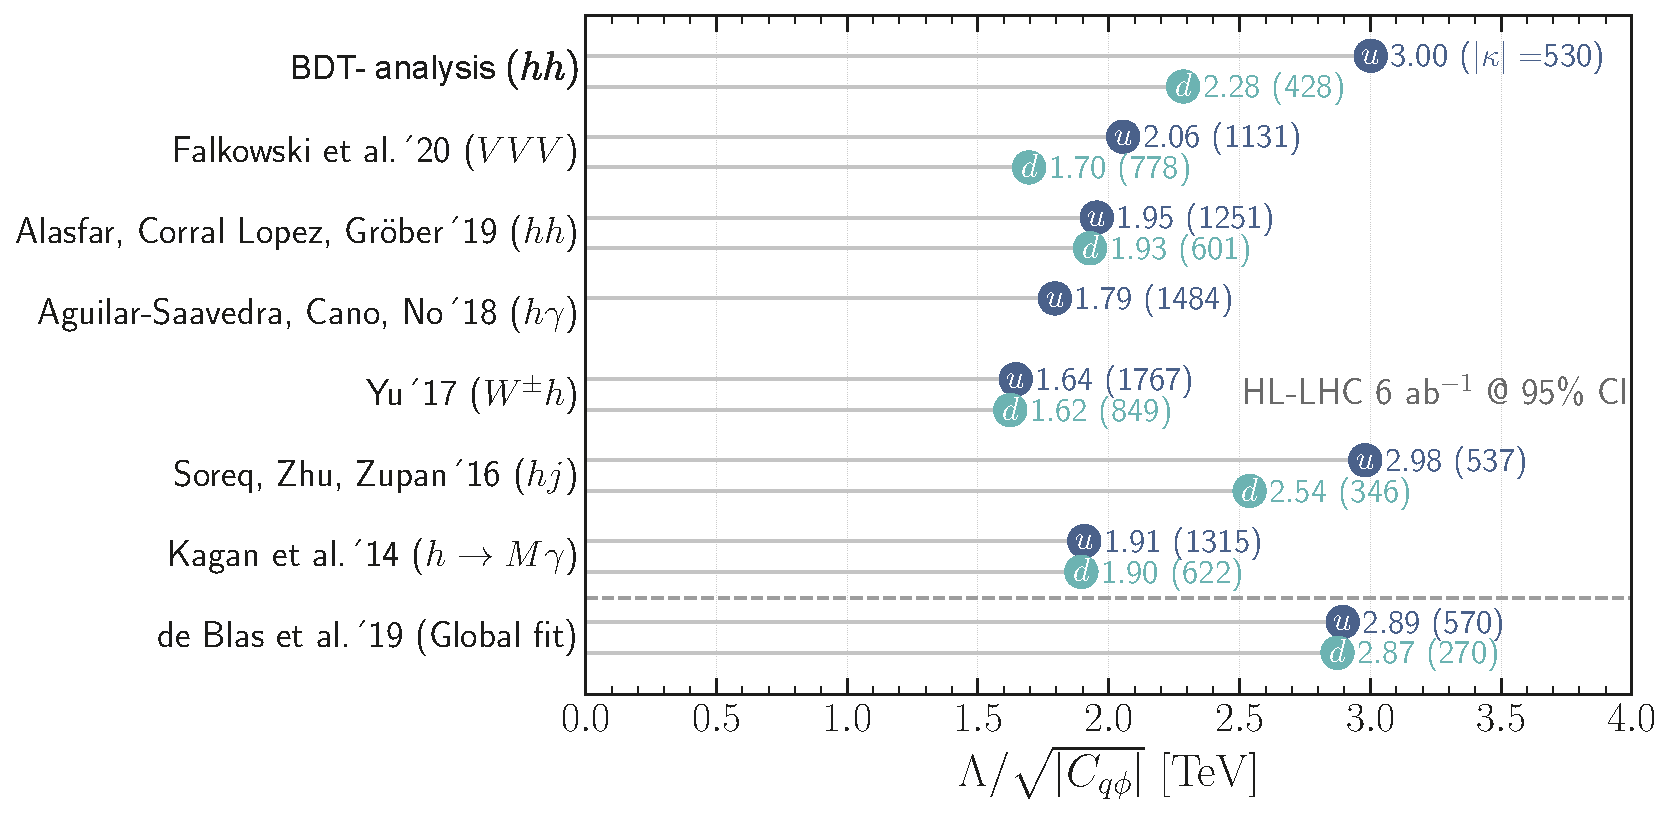
\includegraphics[width=\linewidth]{figures/ueberblick_ly.pdf}
	\caption{Summary of the $95\%$ CI/CL sensitivity bounds on the SMEFT Wilson coefficients $C_{u\phi}$ (blue), and $C_{d\phi}$ (green). The bounds are interpreted in terms of the NP scale $\Lambda$ that can be reached through the measurements of the Wilson coefficient at the HL-LHC at $6$ \invab, the corresponding $\kappa_q$'s are shown inside the parentheses. Single parameter fit $95\%$ CI bounds are used from this analysis for comparison with previous studies.}
	\label{fig:comparison}
\end{figure}

One of the main features of the effective couplings $hh q\bar q$ and $hhh q\bar q$ emerging from SMEFT operator $\mathcal O_{q\phi}$, or the Chiral Lagrangian for that matter, is that these couplings are either free from propagator suppression for $hh q\bar q$ or scale with energy for $hhh q\bar q$ while being safe from strong unitarity constraints. This feature gives processes with multiple Higgs and/or vector bosons $V= W^\pm, Z$ an advantage in constraining $\mathcal O_{q\phi}$. The latter constrains come from the longitudinal degrees of freedom of the gauge bosons  which can be understood from the Goldstone boson equivalence theorem. The use of the final state $VV$ as a probe for $\mathcal O_{q\phi}$ is difficult due to the large SM background. However, the three-boson final state $VVV$ was shown to give strong projected bounds for light-quark Yukawa couplings for HL-LHC with 95\% CL bounds on $\kappa_u \sim 1600$, and $\kappa_d\sim 1100$. A ten fold improvement is expected at FCC-hh~\cite{Falkowski:2020znk} with bounds of order $\kappa_d\sim 30$. 
Higgs pair production has a smaller SM background compared to $VV$ production, but it has a significantly smaller cross section too, even when compared to $VVV$, as the latter process has already been observed at the LHC~\cite{Sciandra:2688061,CMS-PAS-SMP-19-014}.

On the contrary, Higgs pair production is inaccessible with the runs I-III of the LHC, but it is potentially accessible at the HL-LHC~\cite{Binoth:2006ym} having a $ \sigma \cdot BR\sim 1\mathrm{fb}^{-1}$. However, Higgs pair production, particularly the channel $h \to b \bar b \gamma \gamma $, is of significant interest as it has unique features. The first being the ability to constrain the trilinear and light-quark Yukawa couplings simultaneously, as we have already seen in the previous sections. Secondly, Higgs pair production could probe non-linear relations between Yukawa interaction and $hh q\bar q$ couplings~\cite{Contino:2012xk}. Lastly, Higgs pair production is expected to be significant enhanced in certain models involving modification of light-quark Yukawa couplings (cf. ~\cite{Bar-Shalom:2018rjs,Bauer:2017cov,Egana-Ugrinovic:2021uew})

For future colliders, like the FCC-hh at $100$ TeV, in addition to Higgs pair production triple Higgs production might be an interesting channel for constraining the operators with Wilson coefficient $C_{u\phi}$ and $C_{d\phi}$ due to the energy increase of a Feynman diagram coupling the quarks to three Higgs bosons.   In this case, a similar study to ours should be performed to see whether also in this case it will be important to do a combined fit on the light quark Yukawa couplings together with the trilinear and quartic Higgs self-couplings.\footnote{In~\cite{Papaefstathiou:2047255}, it was shown that $\sim \mathcal{O}(1)$ bounds on the quartic Higgs self-coupling can be reached at the FCC-hh.}
Finally, it should be noted that there are also non collider signatures for enhanced light-quark Yukawa couplings, manifesting in frequency shifts in atomic clocks from Higgs forces at the atomic level~\cite{Delaunay:2016brc}. 

\section{Conclusions \label{sec:concly}}

\begin{figure}[!t]
	\centering
	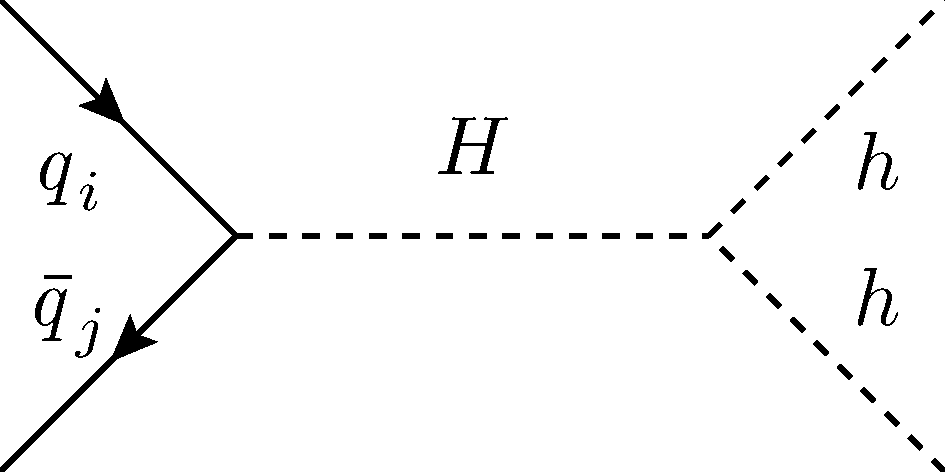
\includegraphics[width = 0.25\textwidth]{./fig/qqh_2hdm}
	\hspace{0.5 cm}
	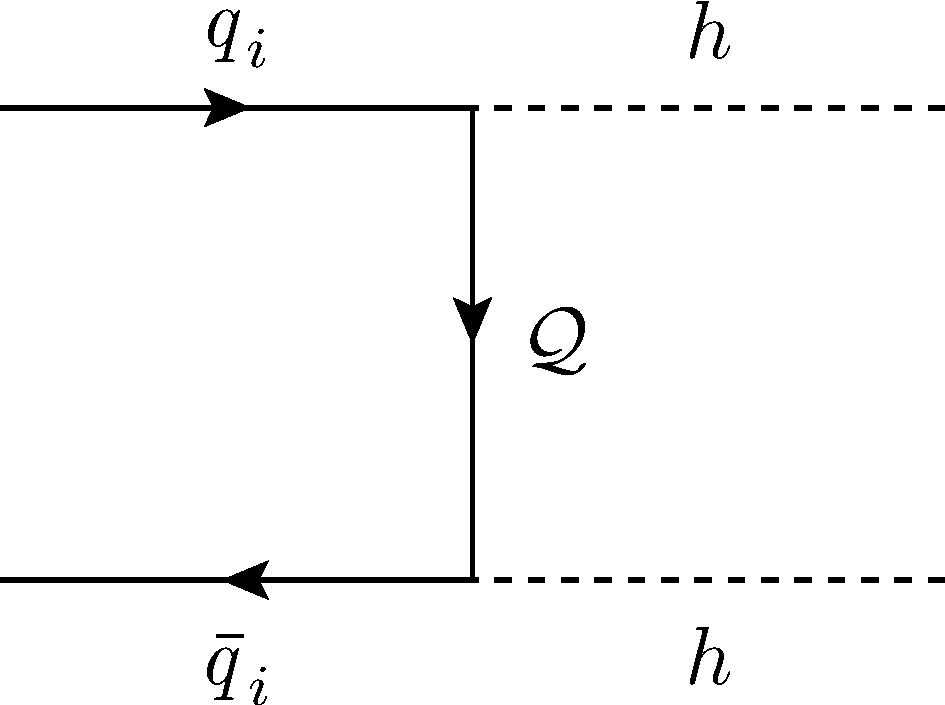
\includegraphics[width = 0.2\textwidth]{./fig/VLQ}
	\caption{Examples of potential UV-complete models leading to a  $hh f \bar{f} $ coupling. The left Feynman diagram shows a heavy Higgs $H$, the right diagram a vector-like quark $\mathcal Q $.} % verify the notation
	\label{fig_uv_qqhh}
\end{figure}


%%%%%%%%%%%%%%%%%%%%%%%%%%%%%
%\section{Phenomenological analysis \label{sec:pheno}}
%In this section we will investigate whether enhanced light quark Yukawa couplings can be measured in Higgs pair production. As we have seen in the previous section,
%we can get an enhancement in the signal strengths for first generation quarks from the enhanced cross sections while BRs in the standard di-Higgs search channels decrease. We have also seen that final states with charm quarks might be worth studying further for enhanced second generation Yukawa couplings.
%Here in this section, we will perform a phenomenological analysis to see if the HL-LHC has potential to constrain the light quark Yukawa couplings in di-Higgs channels.
%The first part of the section is devoted to the analysis strategy, before we discuss the bounds from final states with bottom quarks. We will be  focussing in particular on the $b\bar{b}\gamma\gamma$ final state as it holds promising prospects \cite{Azatov:2015oxa, Baur:2003gp, Baglio:2012np, Kling:2016lay, Barger:2013jfa, Adhikary:2017jtu} despite the low BR of 0.27\% in the SM for the Higgs boson pair. At the end of the section we take a closer look at the $c\bar{c}\gamma \gamma$ final state, which is in particular interesting for enhanced charm Yukawa couplings.
%
%For our phenomenological analysis we do not assume that the efficiency is constant for the new physics hypothesis with respect to the SM efficiency.  Hence, we use the full definition of the signal strength $\mu$ as the ratio of the number of events measured or expected given the new physics hypothesis over the number of events expected by the SM~(null) hypothesis
%\begin{equation}
%	\mu = \frac{ N_{expec}}{ N^{SM}_{expec}}.
%\end{equation}
%The number of expected events $ N_{expec}$ at a hadron collider with integrated luminosity $L$ and selection efficiency $\epsilon_{SEL}$  in the narrow width approximation for a process $pp\to R$ with subsequent decay of $R\to X$ is given by the formula
%\begin{equation}
%	N_{expec} = \sigma(pp\to R) \, \mathcal B(R \to X)\, L \, \epsilon_{\mathrm{SEL}}.
%\end{equation}
%The selection efficiency can be written in terms of several factors by
%\begin{equation}
%	\epsilon_{\mathrm{SEL}} = \epsilon_{\mathrm{Acc}} \cdot \epsilon_{\mathrm{Rec}} \cdot \epsilon_{\mathrm{Trig}}\cdot \epsilon_{\mathrm{cut}},
%\end{equation}
%with $ \epsilon_{\mathrm{Acc}}$ being the detector acceptance efficiency, $ \epsilon_{\mathrm{Rec}}$ the efficiency from reconstruction,  $\epsilon_{\mathrm{Trig}}$ the trigger efficiency and $\epsilon_{\mathrm{cut}}$ the efficiency obtained from the applied kinematical cuts on the signal. For the ATLAS and CMS experiments, the acceptance for the Higgs pair production is close to $100 \%$ due to the complete coverage of the pseudorapidity range of~$2.5< |\eta |< 5$, so we use $\epsilon_{\mathrm{Acc}}=1$.
%The other efficiencies will be discussed in more detail in subsect.~\ref{sec:analysisstrategy}.
%%%%%%%%%%%%%%%%%%%%%%%%%%%%%%%%%%%%%%%%%%%%%%%%%%%%%%
%\subsection{Event generation}
%The parton showering and hadronisation of the process $pp \to hh \to b \bar b \gamma \gamma$ has been simulated using \texttt{Pythia} 6.4~\cite{Sjostrand:2006za} with the settings detailed in appendix~\ref{app:pythia}. The cross section of the Higgs pair production (ggF and qqA both at LO multiplied by a $K$-factor as described in subsect.~\ref{sec:ggF} and \ref{sec:qqA_NLO}) is fed to \texttt{Pythia} which decays the two Higgs bosons and then performs the parton showering. We have accounted for the correct BRs by using the values obtained as described in subsect.~\ref{sec:Hdecay} from \texttt{ HDECAY}. We have turned on initial and final state QCD and QED radiation and multiple interactions.  \\
%The generated events were written to a ROOT file via \texttt{RootTuple} tool~\cite{roottuple} for further analysis.
%%%%%%%%%%%%%%%%%%%%%%%%%%%%%%%
%\subsection{Analysis strategy \label{sec:analysisstrategy}}
%The analysis strategy follows the one performed in~\cite{Azatov:2015oxa} allowing us to use their backgrounds. Note that the analysis was based on the SM  simulated events, meaning that the significances could be potentially improved performing a dedicated new physics analysis.
%In order to satisfy the minimal reconstruction requirements of the LHC we select only events with
%\begin{equation}
%	p_T(\gamma/j) > 25 \, \GeV\,, \; \; \; \; |\eta(\gamma/j)| < 2.5\,.
%\end{equation}
%Moreover, we veto events with hard leptons
%\begin{equation}
%	p_T(\ell) > 20 \, \GeV, \; \; \; \; |\eta(\ell)| < 2.5\,,
%\end{equation}
%corresponding of an expected $ \epsilon_{\mathrm{Trig}}=0.9$.
%Jets were clustered using \texttt{fastjet}~\cite{Cacciari:2011ma}  with the anti-kt algorithm with a radius parameter of $R=0.5$. \\
%We have used a $b$-tagging efficiency of $ \epsilon_b = 0.7$ \footnote{We have explicitly cross checked the number by doing a mass-drop tagger analysis \cite{Butterworth:2008iy}.}.
%The contamination probability of $\epsilon_{j \to b} < 1 \%$  is found to be consistent with ATLAS and CMS performance~\cite{Chatrchyan:2012dk,CMS:2013vea,ATL-PHYS-PUB-2013-009}. For the photon reconstruction efficiency  we used $ \epsilon_\gamma = 0.8$ as reported by ATLAS and CMS in~\cite{ATL-PHYS-PUB-2013-009,CMS:2013aoa}.
%The selection cuts we used are the same ones as in~\cite{Azatov:2015oxa}, starting with the cuts of the transverse momentum $p_T$ of the photons and $b$-tagged jets. The two hardest photons/$b$-tagged jets,  with transverse momentum $p_{T>}$, and the softer ones with $p_{T<}$ are selected to satisfy
%\begin{equation}
%	p_{T>}(b/ \gamma) > 50 \, \GeV, \quad \text{and} \quad   p_{T<}(b/ \gamma) > 30 \, \GeV\,.
%	\label{cut1}
%\end{equation}
%%
%In order to ensure well-separation of the photons and $b$-jets, we require the following cuts on the jet radius,
%% new plots
%\begin{equation}
%	\Delta R(b,b) < 2  ,\; \; \; \; \Delta R(\gamma,\gamma) < 2, \; \;  \; \; \Delta R(b,\gamma) > 1.5\,.
%	\label{cut2}
%\end{equation}
%While the majority of the signal lies within this region, these cuts significantly reduce the backgrounds.
%
%We choose a wide $m_{\gamma \gamma}$  window (see eq.~\eqref{cut3}) corresponding to 2-3 times the photon resolution of ATLAS and CMS~\cite{ATL-PHYS-PUB-2013-009,CMS:2013aoa} which does not cause any significant loss. As for the Higgs  mass window reconstructed from 2 $b$-jets $ m_{b\bar b}$, the mass window chosen in eq.~\eqref{cut3} corresponds to the given $b$-tagging efficiency. The mass windows used are then
%% \Lina{If you use the truth-level b- jets as b-tagged ones, without a mass window, this gives $\epsilon_b = 1$, However, the $m_{bb}$ mass window gives approx. the correct b-tagging efficiency. The mass window is not efficiency is not included in the cuts efficiency. Typically in experimental analysis they use a narrower window.  The mass window on $m_{\gamma \gamma}$ corresponds to the detector resolution not particle identification in the EM calorimeter, $\epsilon_\gamma$ is for the identification not resolution. }
%\begin{equation}
%	105\,\GeV < m_{b \bar b} < 145 \, \GeV, \; \; \; \;123\, \GeV < m_{\gamma \gamma} < 130 \, \GeV\,.
%	\label{cut3}
%\end{equation}
%The selection cuts are summarised in table~\ref{cuts_eff} with their corresponding efficiency. In table~\ref{eff} we summarise all the efficiencies used in the analysis.
%
%\begin{table}[!t]
%	\centering
%	\begin{tabular}{l cc }
%		\toprule
%		cut  & $\epsilon_{\mathrm{cut}}$  &  $ \delta \epsilon_{\mathrm{cut}}$  \\
%		\midrule
%		$p_T$ cuts in eq.~\eqref{cut1} & 0.35 & 0.07\\
%		$\Delta R$ cuts  in eq.~\eqref{cut2} & 0.69 & 0.21 \\
%		% Higgs mass windows in~\ref{cut3} & \eff{13}{14} & \poiserr{13}{18} \\
%		\hline
%		total    & 0.16 & 0.05 \\
%		\bottomrule
%	\end{tabular}
%	\caption{The cuts used in the analysis with their efficiency $\epsilon_{\mathrm{cut}}$ and uncertainties on these efficiencies $ \delta \epsilon_{\mathrm{cut}} = \sqrt{\epsilon(1-\epsilon)\,N}$, where $N$ is the total number of events. The analysis was performed on 100K SM simulated events.}
%	\label{cuts_eff}
%\end{table}
%\begin{table}[!t]
%	\centering
%	\begin{tabular}{ c c }
%		\toprule
%		Type & efficiency \\
%		\midrule
%		$\epsilon_{\mathrm{Acc}}$  & $\sim 1$ \\
%		$\epsilon_{\mathrm{Rec}}$ & 0.31 \\
%		$\epsilon_{\mathrm{Trig}}$ & 0.90 \\
%		$\epsilon_{\mathrm{Cut}}$ & 0.16 \\
%		\hline
%		total    &  0.044\\
%		\bottomrule
%	\end{tabular}
%	\caption{Values of the efficiencies calculated/used in this analysis. }
%	\label{eff}
%\end{table}
%\par
%The major backgrounds for the considered final state are the $b\bar{b}\gamma\gamma$ continuum background, $\gamma\gamma jj$ with two mistagged jets, $t\bar{t}h$, $Zh$ and $b\bar{b}h$ in the order of importance after the cuts in eq.~\eqref{cut1}. The number of background events (surviving the cuts) is taken from~\cite{Azatov:2015oxa}. The backgrounds are illustrated in the fig.~\ref{sm_hh_and_bkg} in which we show the number of events for the SM Higgs pair signal in light blue and the most relevant backgrounds in other colors. It should be noted that the background $h(\to \gamma \gamma) Z(\to b \bar b)$  is modified in the presence of enhanced light quark Yukawa couplings. We checked though explicitly that scaling the Yukawa couplings to the values of our benchmark point only changes the NLO cross section by less than 1\%, making this effect negligible.
%%
%The analysis was carried out for varying values of $\kappa_f$ for the different flavours. Due to the change in the kinematical distributions (cf.~fig.~\ref{eff_ratio}) resulting from the PDFs of the different flavours, the efficiencies depend on the flavour of the quarks.
%For $\kappa_f\gg 1$ the $\kappa_f$ dependence factors out of the cross section such that for the values considered in the analysis of the distributions no dependence on the concrete value of $\kappa_f$ is seen. The flavour-specific efficiency ratio~$\epsilon_f$ is given by
%\begin{equation}
%	\epsilon_f =  \frac{\sigma_{ggF} \, \epsilon_{ggF} + \sigma_{q\bar q}  \, \epsilon_{qq} }{\sigma_{gg} + \sigma_{q\bar q}}\,,
%	\label{effrat}
%\end{equation}
%with $\sigma_{ggF}$ being the gluon fusion cross section, $\sigma_{q\bar q}$ the quark annihilation cross section and $\epsilon_{ggF} = 0.044$. We give the values for the qqA efficiency $\epsilon_{qq}$ in table~\ref{eps_vark}.
%\begin{table}[!b]
%	\centering
%	\begin{tabular}{cc}
%		\toprule
%		$\delta \kappa$ 	& $ \epsilon_{qq}$	 \\
%		\midrule
%		$\kappa_{u}$   & $0.050$  \\
%		$\kappa_{d}$   & $0.049$   \\
%		$\kappa_{u}$ \& $\kappa_{d}$   & $0.053$  \\
%		\hline
%		$\kappa_{c}$   & $0.034$  \\
%		$\kappa_{s}$   & $0.037$   \\
%		$\kappa_{c}$ \& $\kappa_{s}$   & $0.039$  \\
%		\bottomrule
%	\end{tabular}
%	\caption{The dependence of $\epsilon_{qq}$ on the flavour of the Yukawa couplings' scalings.}
%	\label{eps_vark}
%\end{table}
%
%In fig.~\ref{eff_ratio} we show for the SM and for our benchmark point $g_{hq\bar{q}}=g_{hb\bar{b}}^{\text{SM}}$ the $M_{hh}$ distribution. The lower panels in the plot show the efficiencies. These plots illustrate how the efficiency depends on the shape of the distribution, and hence the flavour~$f$ that is scaled by $\kappa_f$.
%
%%
%\subsection{Statistical analysis}
%We have used the likelihood ratio test statistic~$q_\mu$ in order to estimate the HL-LHC sensitivity, and set projected limits on the scalings of the light Yukawa couplings. A (log)--likelihood was constructed from the signal and background events in each bin of the histogram in fig.~\ref{sm_hh_and_bkg},
%\begin{equation} \label{loglik}
%	- \ln \mathscr L (\mu) = \sum_{i \in \mathrm{bins}} (N_{bi} + \mu\, N_{si}) - n_i\, \ln(N_{bi} + \mu\, N_{si}),
%\end{equation}
%with  $N_{bi}$ and $N_{si}$ being the number of background  and signal events in the $i$th $ M_{hh}$ distribution, respectively. In order to include the theoretical uncertainties on the expected number of signal events, the above likelihood was extended by a gaussian distribution for $N_{si}$ in which the mean equals to the central value of the bin values and standard deviation $\sigma$ equals to its theoretical uncertainty.
%The signal strength $ \mu$ was then estimated by minimising $- \ln \mathscr L (\mu)$ to obtain the estimator for $\hat \mu$ by injecting SM signal + background events $n_i$. The test statistic is then given by
%\begin{equation}
%	q_\mu = 2 (\ln \mathscr L (\mu)- \ln \mathscr L ( \hat \mu) ),
%\end{equation}
%following the procedure described in~\cite{Cowan:2010js}.
%\par
%In order to set bounds on the scalings, we have fitted the signal strength inclusively by a function depending on the scaling of the Yukawa couplings
%\begin{equation}
%	\mu(\kappa_1,\kappa_2) = \Bigg\{ \frac{1}{Z}\,\left[ A_0\,
%	\left(
%	\kappa_1^2 \frac{m_{q1}^2}{M_{hh}^2} \, \ln^2\left(\frac{M_{hh}}{m_{q1}} \right) \right)+ A_1\,\left(\kappa_2^2 \frac{m_{q2}^2}{M_{hh}^2} \, \ln^2 \left(\frac{M_{hh}}{m_{q2}} \right)
%	\right)
%	\right] + B_2 \Bigg\}\, \epsilon_f,
%	\label{modelmu}
%\end{equation}
%with
%\begin{equation}
%	Z = \frac{\kappa_1^2 \, m_{q1}^2 +\kappa_2^2 \, m_{q2}^2  + B_0}{m_{q1}^2+m_{q2}^2+ B_1}
%\end{equation}
%and $m_{q1}$ and $m_{q2}$ denoting the $\bar{\text{MS}}$ masses of the quarks.
%% In table~\ref{eps_vark}
%
%
%Taking $M_{hh} \approx 300$ GeV, we could perform a fit for the signal strength for each of the quark generations scalings separately. Note that one could of course also extend the model to include the dependence of the signal strength on four Yukawa coupling modifications, taking into account the correlation between them when fitting the likelihood in eq.~\eqref{loglik}.
%
%The expected HL-LHC sensitivity for the signal strength  at 95\% (68 \%) CL is found to be $\mu  = 2.1 (1.6)$.
%\par
%\subsection{Results for the $b\bar{b}\gamma\gamma$ final state}
%We have performed a scan on the first generation Yukawa coupling scalings $ \kappa_u$ and $ \kappa_d$ in order to obtain exclusion limits, derived from the likelihood contours shown in fig.~\ref{bounds_1stgen}. The individual $\kappa_q$ expected upper bounds at 68\% and 95\% CL are obtained by profiling the likelihood over the other first generation $\kappa_q$.  Doing so, we obtain the following upper bounds for HL-LHC
%\begin{equation}
%	-571  < \kappa_d <  575, \;(\text{68\% CL}), \, \;\;\;\; \,
%	-853 < \kappa_d <  856,\;(\text{95\% CL}),
%\end{equation}
%and %
%\begin{equation}
%	-1192  < \kappa_u < 1170, \;(\text{68\% CL}), \, \;\;\;\; \,
%	-1771 < \kappa_u <  1750,\;(\text{95\% CL}).
%\end{equation}
%
%\begin{figure}[!b]
%	\centering
%	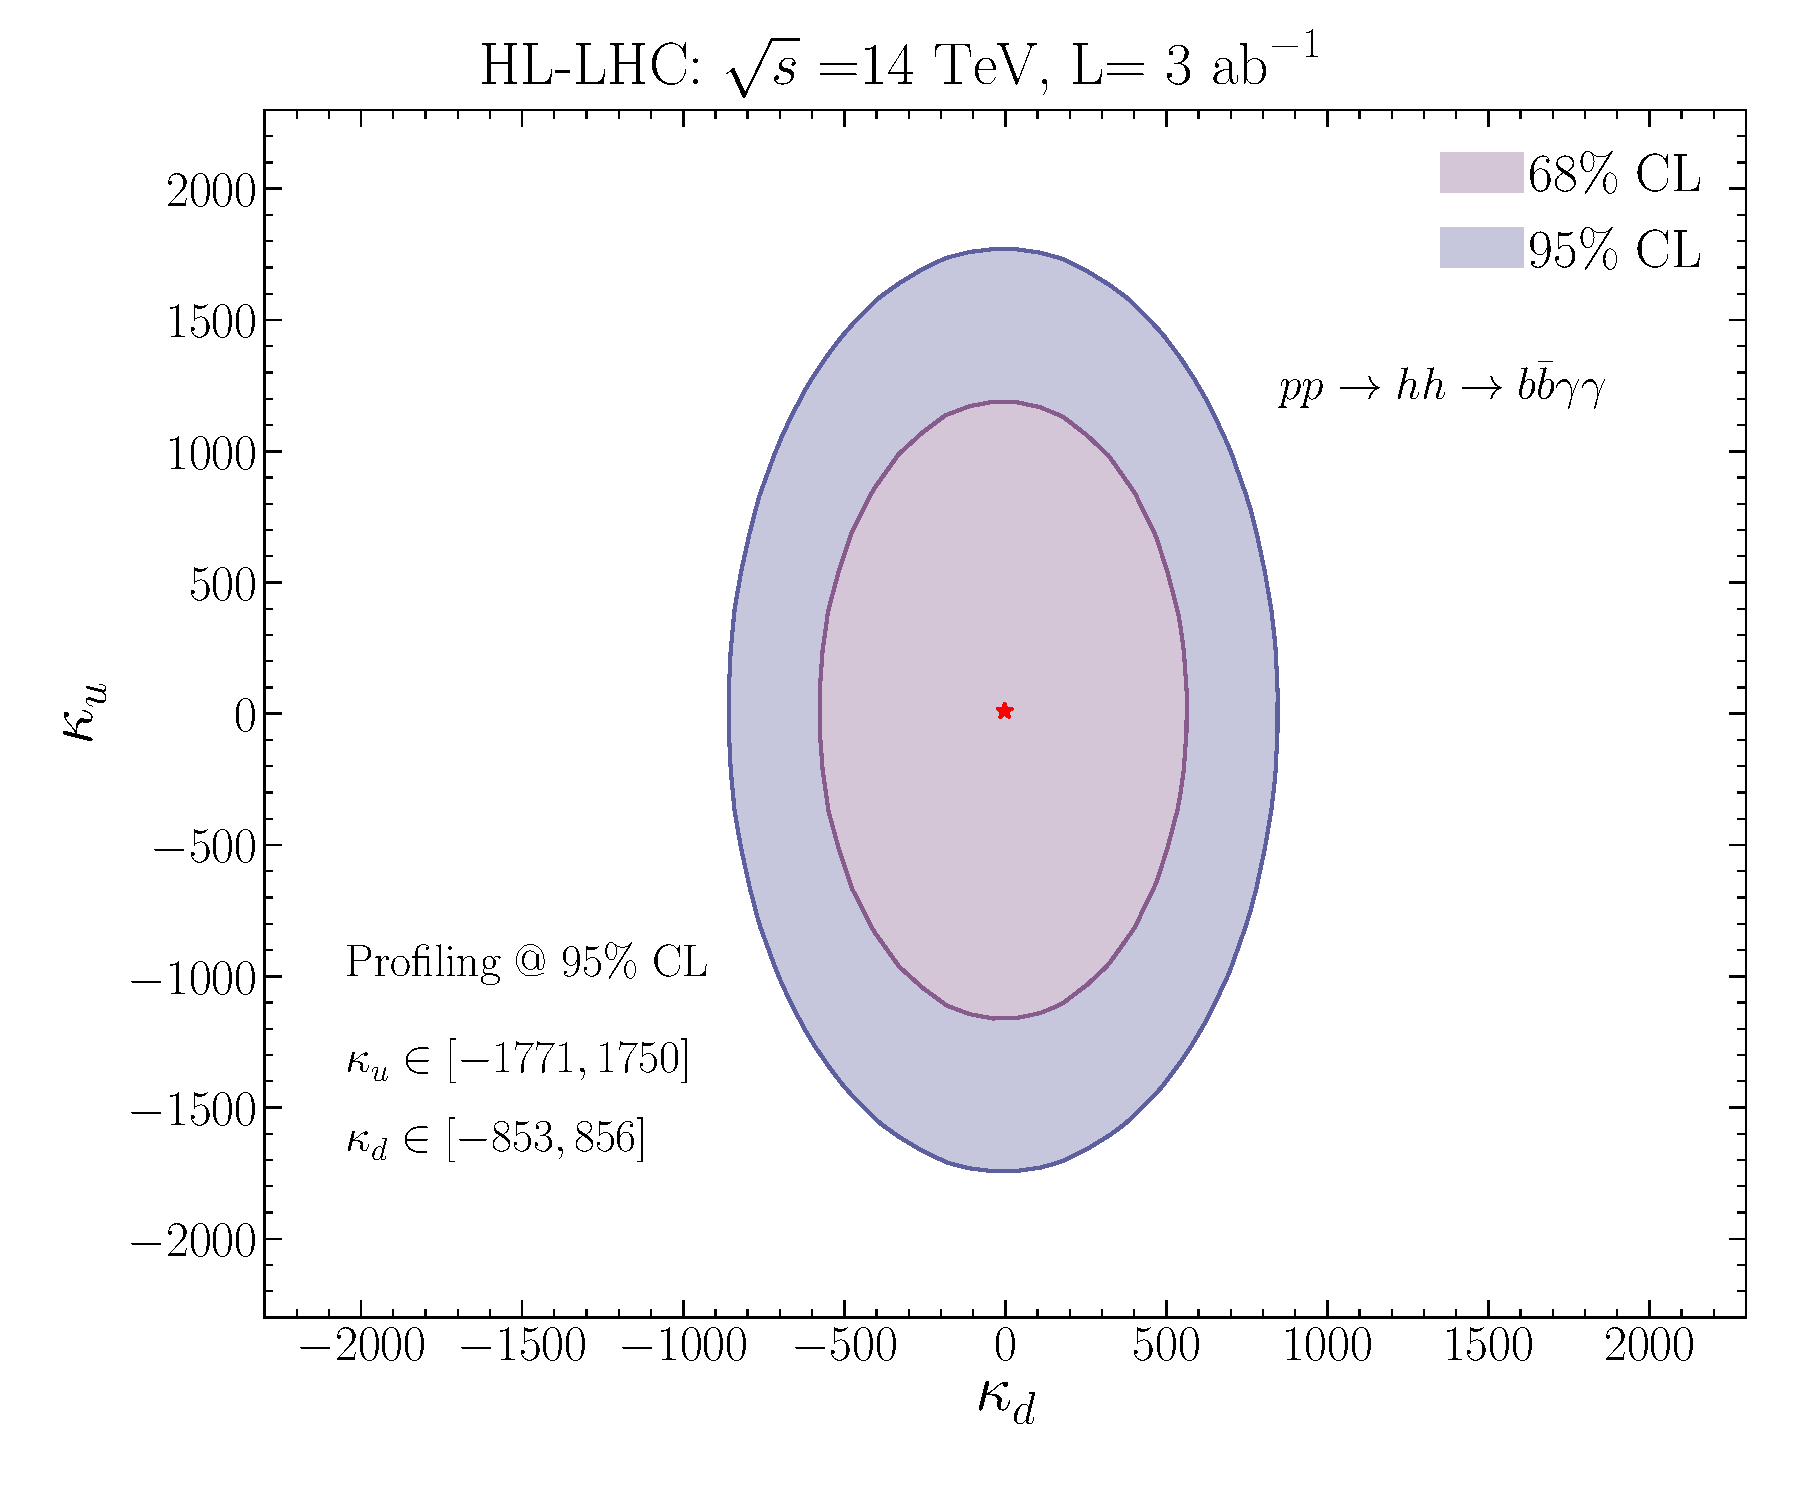
\includegraphics[width = 0.75\textwidth]{./fig/1st_gen_exclusion}
%	\caption{The expected sensitivity likelihood contours  at  68\% and 95\% CL of the HL-LHC for the first generation Yukawa coupling scalings. }
%	\label{bounds_1stgen}
%\end{figure}
%%
%\par
%Note that these bounds are not directly comparable to the standard $\kappa$ formalism bounds since we relate with $\kappa$ the Yukawa couplings $g_{hq\bar{q}}$ and the new coupling  $g_{hhq\bar{q}}$.
%For the second generation quarks we were not able to obtain similar bounds due to the reduction of ~$\mu /\mu_{\SM}$ with increasing $ \kappa_s$ and $\kappa_c$ away from the SM, which stems from the decrease of the branching ratio $\mathcal B (hh \to b \bar b \gamma \gamma)$ as new decay channels open, while the cross section is not as much enhanced as for up and down quarks due to the charm and strange quark being less abundant in the proton. This leads to signal strength modifiers $\mu/\mu_{\SM}< 1$ (\textit{cf}.~fig.~\ref{kcks_mu_contors}).  We will analyse the second generation Yukawa couplings instead for the final state $hh \to c \bar c \gamma \gamma$, in which we observe significant enhancement of the relative signal strength modifier $\mu/\mu_{\SM}$ (\textit{cf}.~fig.~\ref{kcks_mu_contors}). Before turning to a different final state though, we will reanalyse the $b\bar{b}\gamma\gamma$ final state under the point of view of a non-linear effective field theory, hence leaving the couplings $g_{hq\bar{q}}$ and $g_{hhq\bar{q}}$ independent.
%%%%%%%%
%\subsubsection{Results for non-linear EFT}
%We will consider in this part a non-linear EFT as introduced in eq.~\eqref{chirallag}. By expanding in the chiral modes, taking the 0th mode and the flavour diagonal terms, we get
%\begin{equation}
%	-\mathcal L = \bar q_{L} \frac{m_q}{v} \left( v + c_{q}h + \frac{c_{qq}}{v} h^2 + \dots \right) q_R + h.c,
%\end{equation}
%where we rescaled the coefficients $k_{q}$ and $k_{2q}$ of eq.~\eqref{chirallag} as  $ k_{q,ii} =\sqrt{2}  c_{q} m_q/v $ and $ k_{2q,ii} =\sqrt{2}  c_{qq}m_q/v^2 $.  Unlike the linear EFT, the Wilson coefficients $c_{q}$ and $ c_{qq}$ are independent of each other. Using the previous analysis,  it is possible to set bounds on these coefficients separately, as seen in fig.~\ref{nleft}.
%\begin{figure}[!ht]
%	\centering
%	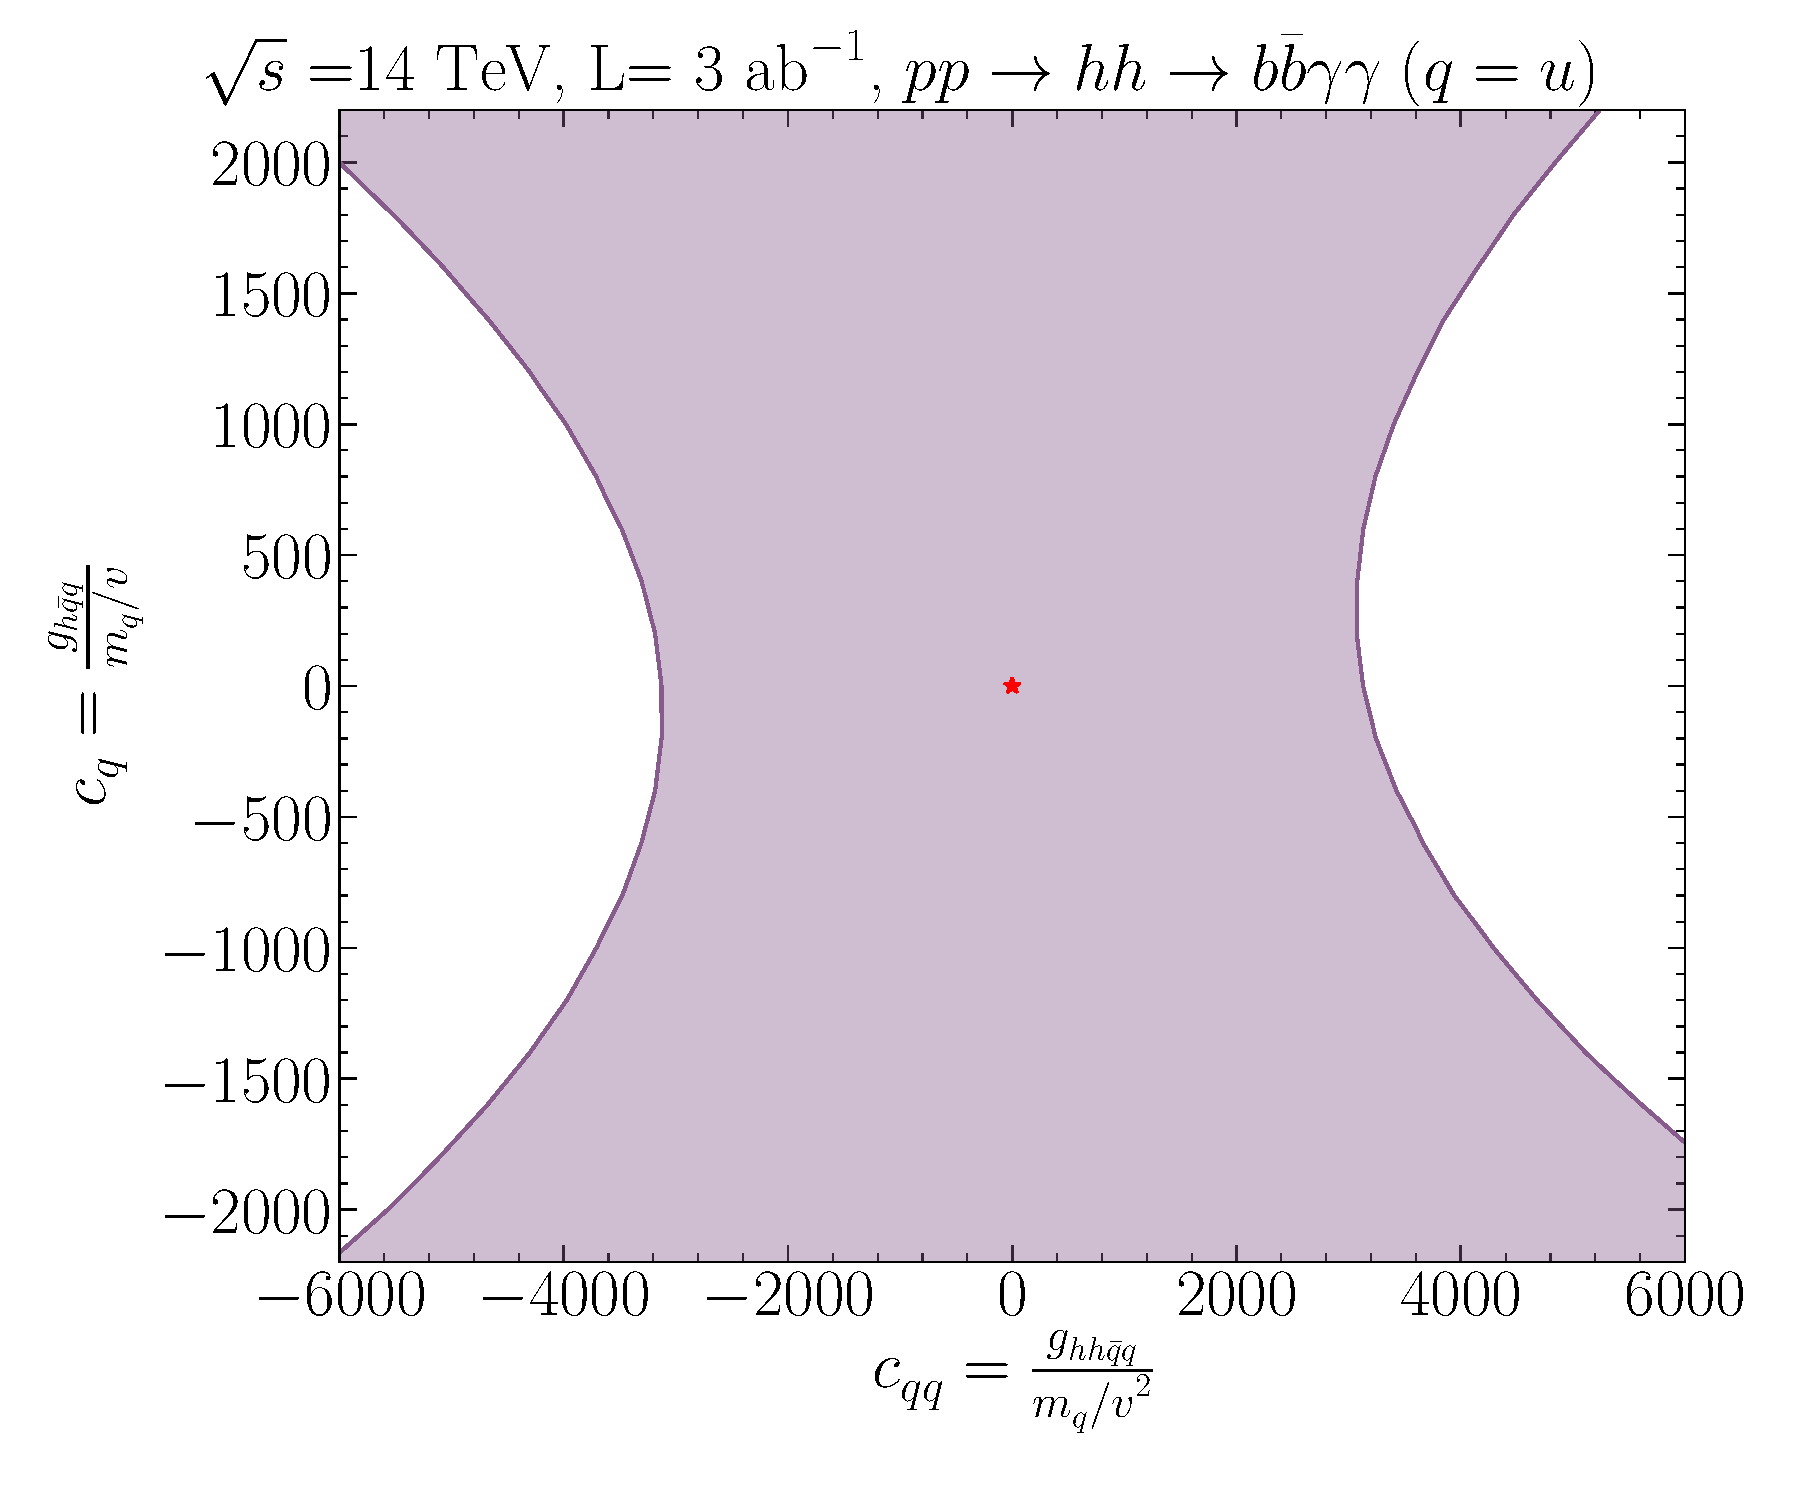
\includegraphics[width = 0.49\textwidth]{./fig/up_nleft}
%	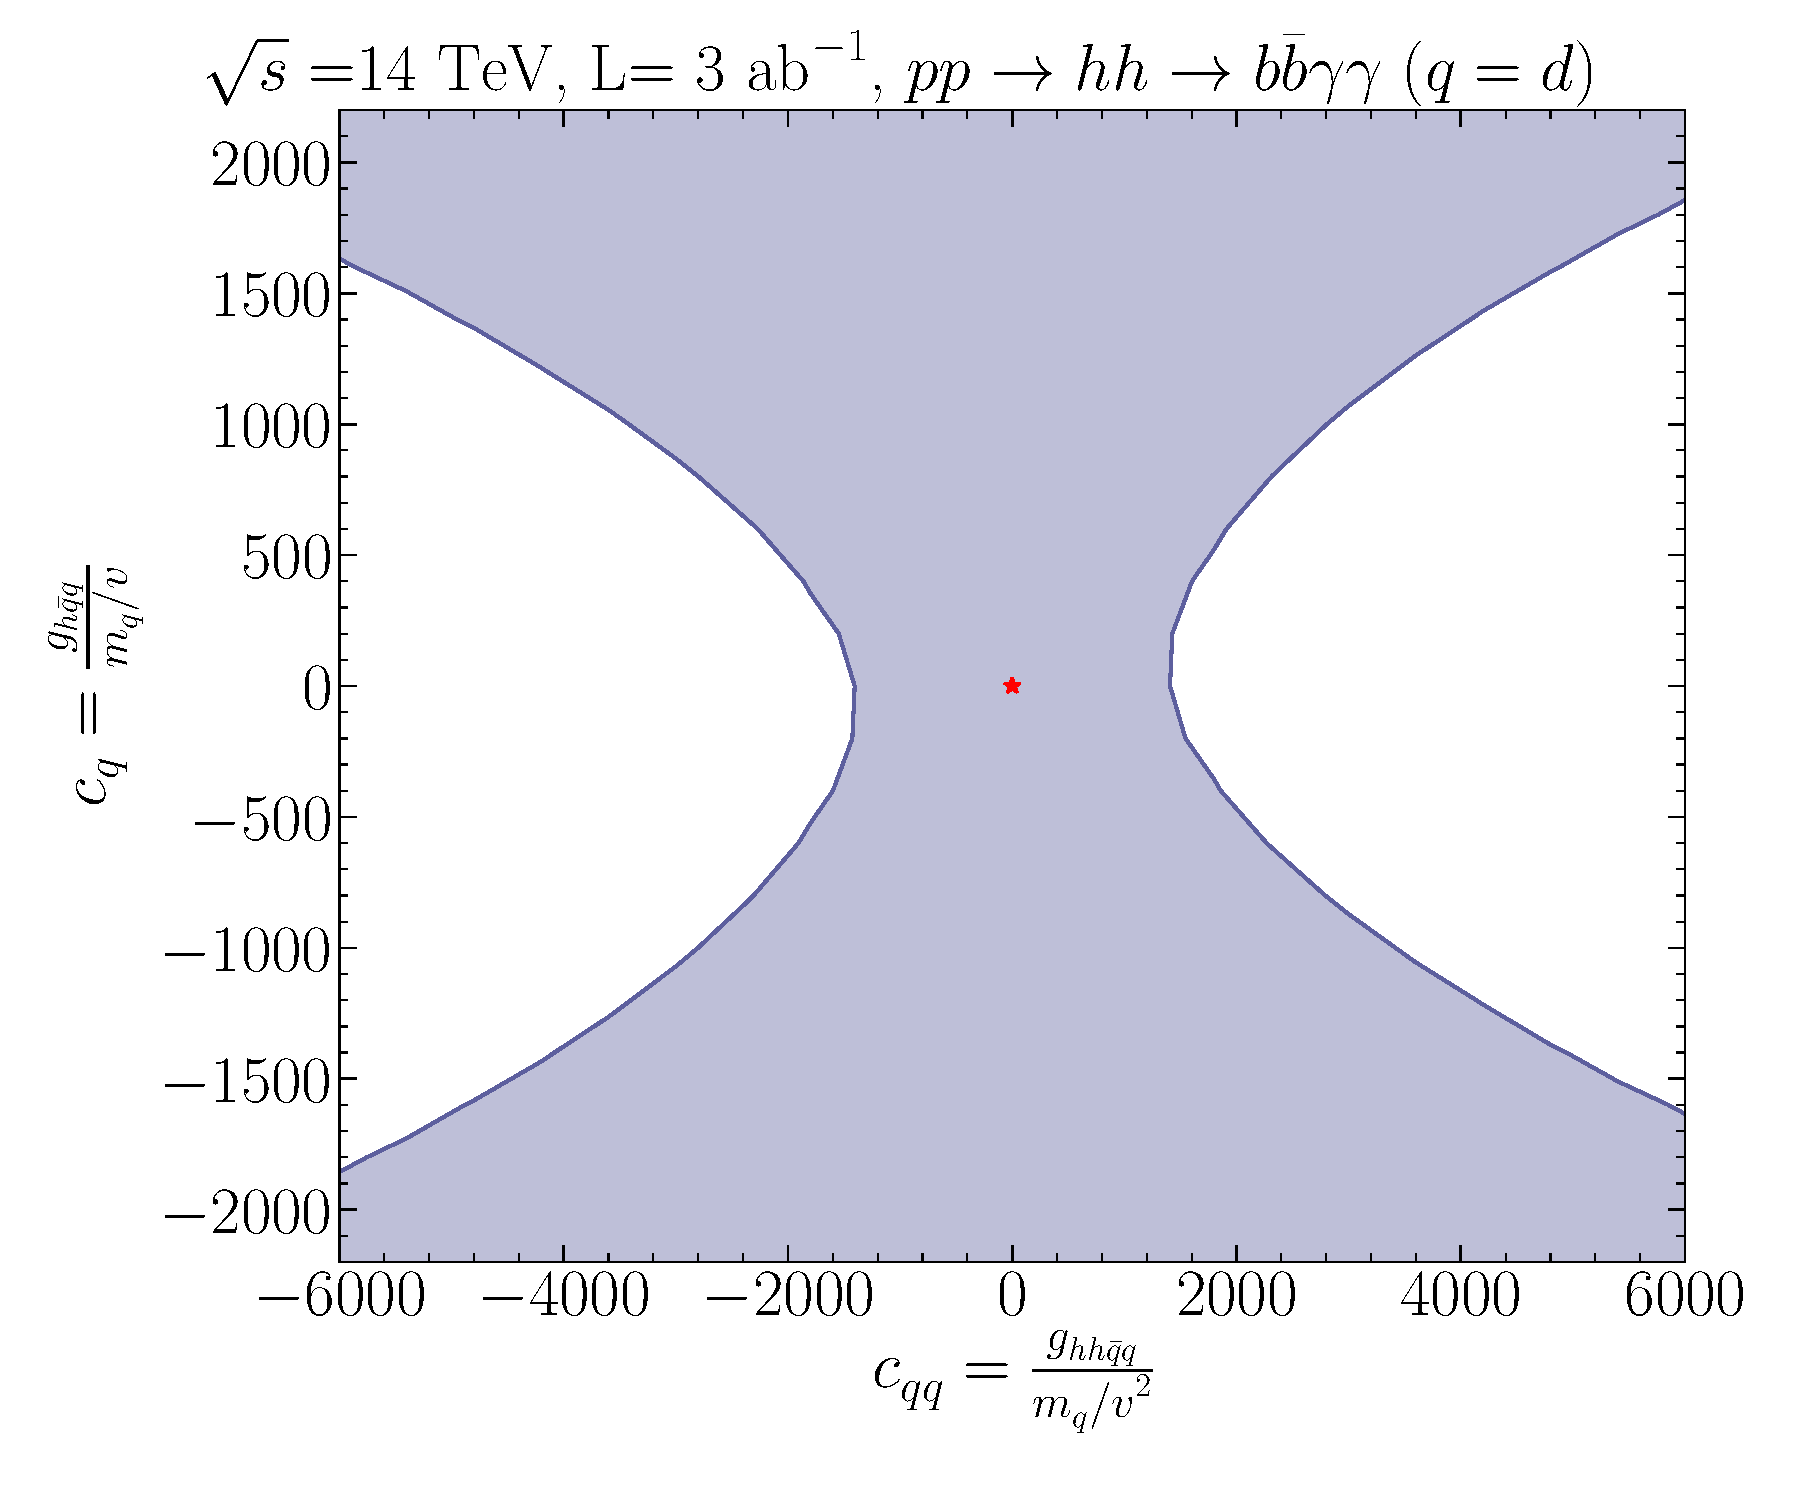
\includegraphics[width = 0.49\textwidth]{./fig/down_nleft}
%	\\
%	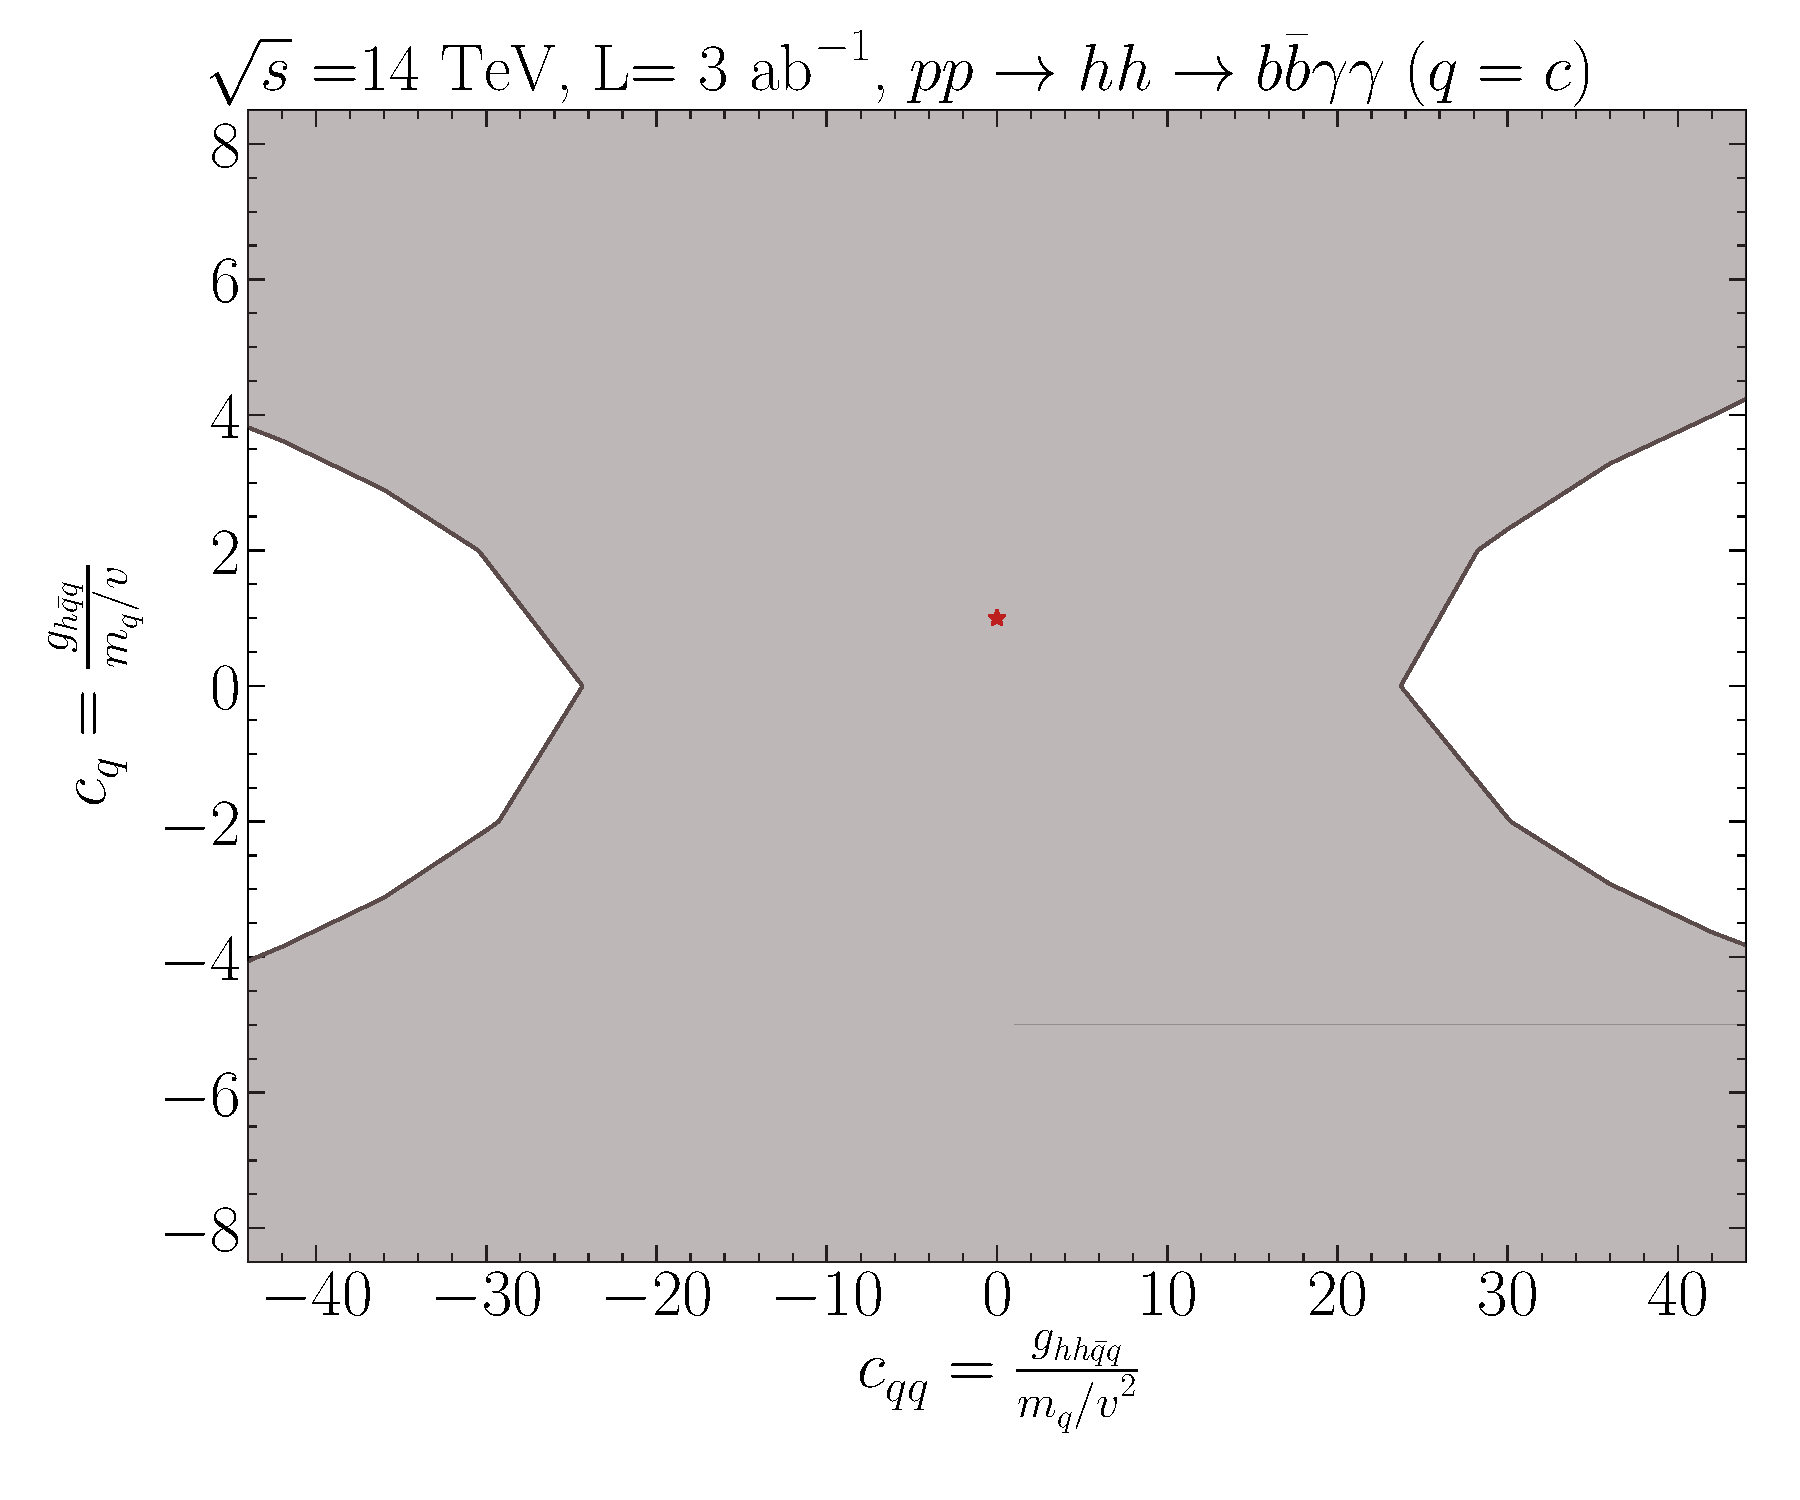
\includegraphics[width = 0.49\textwidth]{./fig/charm_nleft}
%	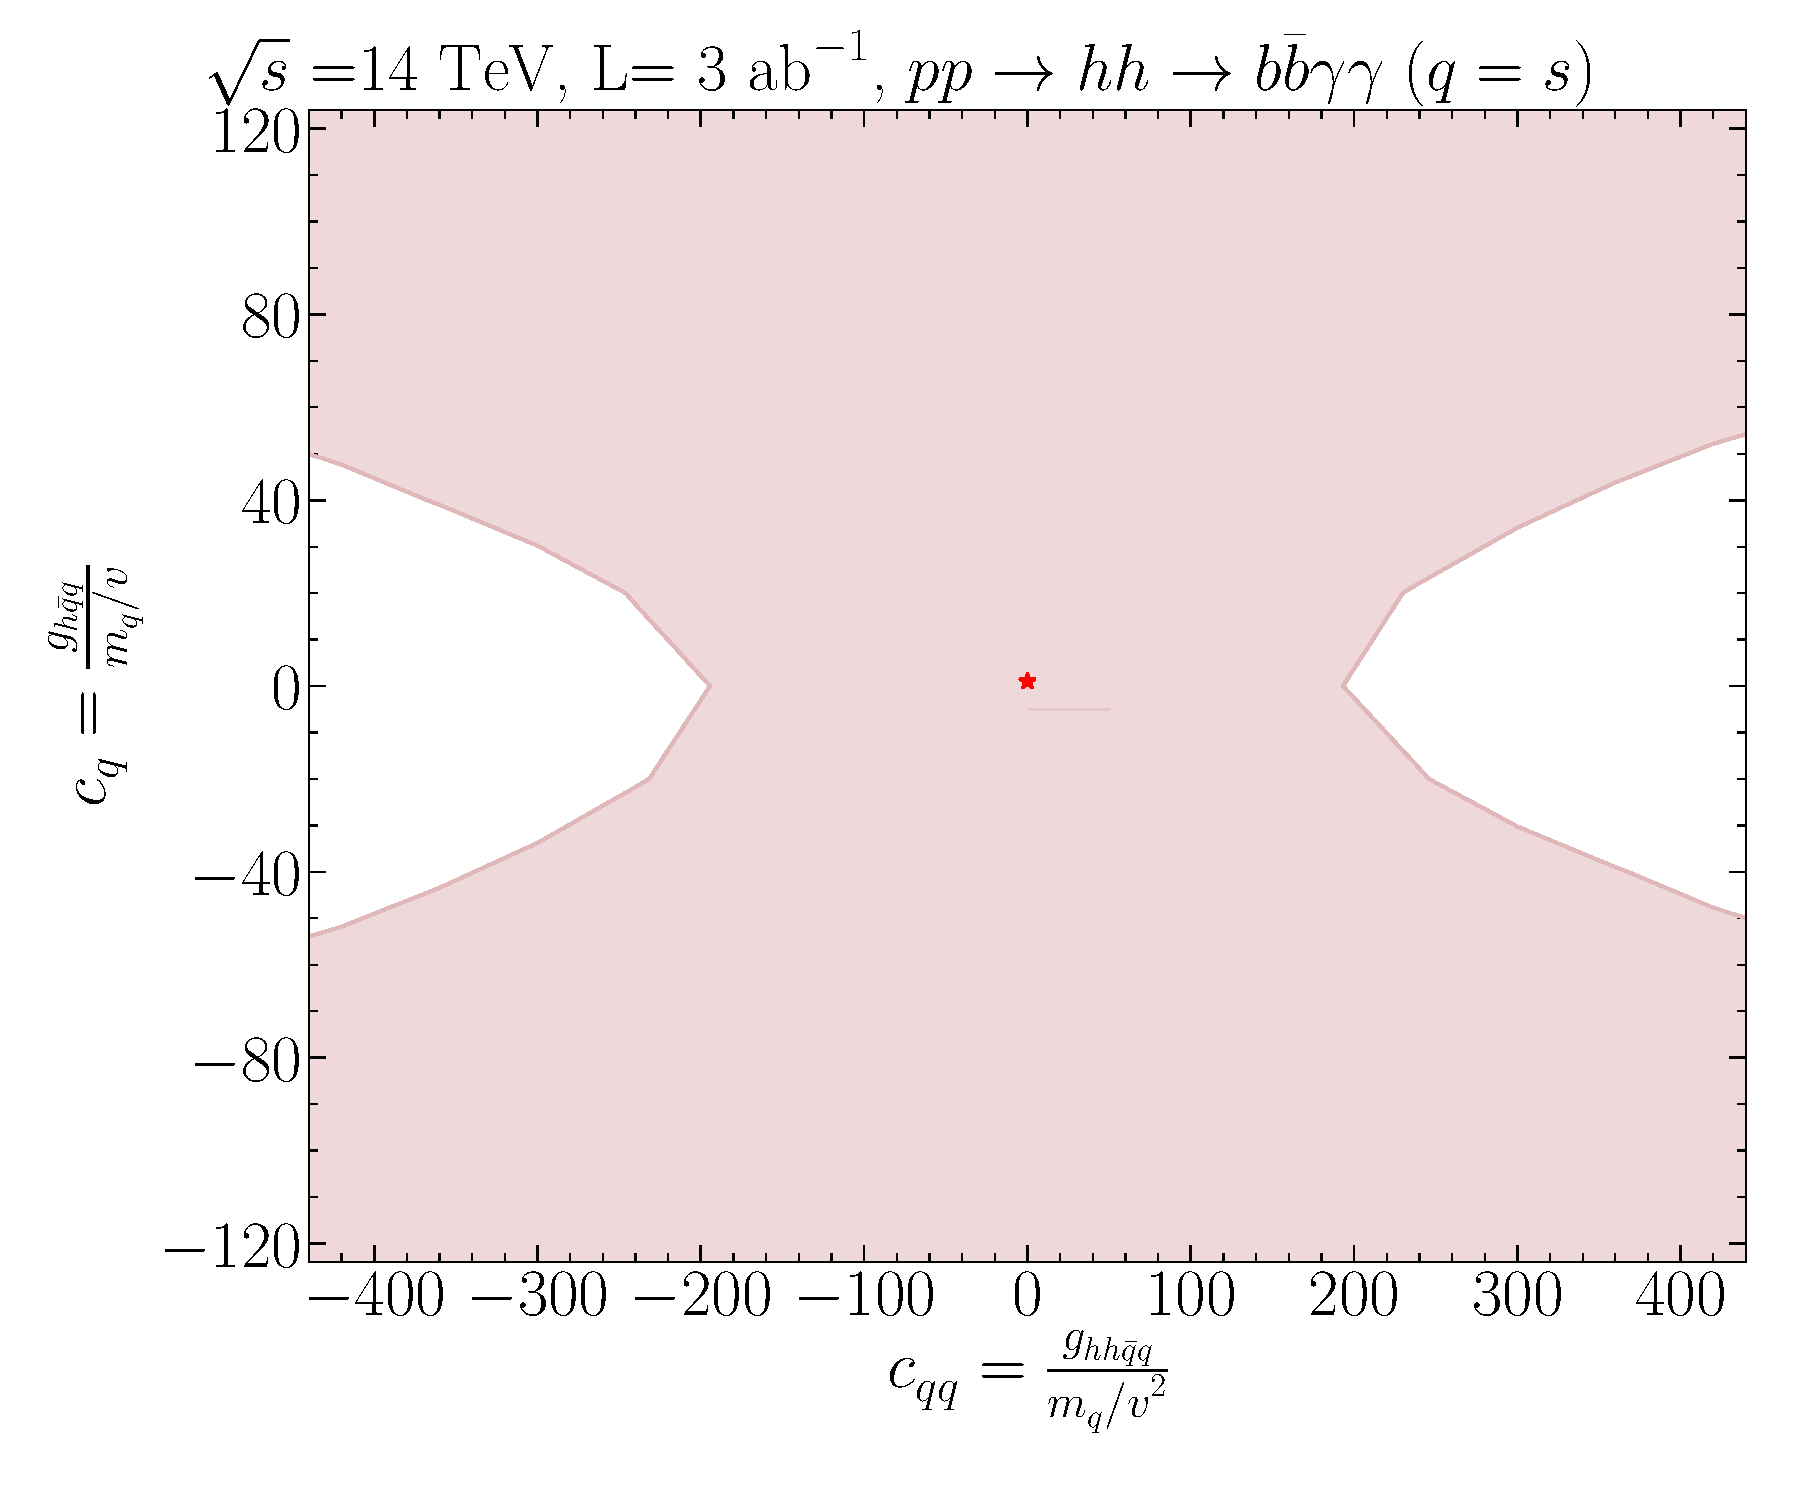
\includegraphics[width = 0.49\textwidth]{./fig/strange_nleft}
%	\caption{95\% CL likelihood contours for the non-linear EFT Wilson coefficients $c_{qq}$ and $ c_{q}$ for up  (\textit{upper left}), down  (\textit{upper right}), charm (\textit{lower left}) and strange quarks (\textit{lower right}).}
%	\label{nleft}
%\end{figure}
%We observe that without the $hh \bar q q$ interaction, one cannot set bounds on any of the light Yukawa couplings from Higgs pair production. We remark though that in case any deviation in the light Yukawa couplings is observed, the di-Higgs channel can distinguish whether electroweak symmetry breaking is realised linearly or non-linearly.
%%%%%%%%%%%%%%%%%%%%%%%%%%%%%%%%%%%%%%%%%%%%%%%%%%%%%
%\subsection{Charm-tagging and second generation bounds}
%In order to set bounds on the second generation Yukawa couplings, we use the method developed in~\cite{Perez:2015aoa,Kim:2015oua} that re-analyses final states with $b$-quarks based on the mistagging of $c$-jets as $b$-jets in associated $VH$ production. The analysis relies on the current CMS~\cite{Chatrchyan:2013zna} and ATLAS~\cite{Aad:2014xzb} working points for $b$-tagging, as illustrated in the table~\ref{btag_wp}.
%\begin{table}
%	\centering
%	\begin{tabular}{ccc}
%		\toprule
%		Detector	& Cuts (1st, 2nd) $b$-jets	& $\epsilon_{c/b}^{\mathrm{b-tag}\,2}$  \\
%		\midrule
%		CMS    & Med1-Med1   & $0.18$               \\
%		CMS    & Med1-Loose  & $0.23$                \\
%		\hline
%		ATLAS  & Med-Med     & $8.2 \cdot 10^{-2}$ \\
%		ATLAS  & Tight-Tight & $5.9 \cdot 10^{-3}$ \\
%		\bottomrule
%	\end{tabular}
%	\caption{The $b$-tagging working points used in the analysis, for CMS~\cite{Chatrchyan:2013zna} and ATLAS~\cite{Aad:2014xzb}. }
%	\label{btag_wp}
%\end{table}
%The signal strength estimator when considering the mistagging probability  of $b$-jets to $c$-jets~(i.e. $c$-jet contamination of b-tagged jets)~$\epsilon_{b\to c}$ is
%\begin{equation}
%	\hat \mu = \frac{\sigma_{hh}\, \mathcal B_b\ \,\epsilon_{b1}\,\epsilon_{b2} \,\epsilon_f+\sigma_{hh}\, \mathcal B_c \,\epsilon_{b\to c,1} \,\epsilon_{b\to c,2}\,\epsilon_f }{\sigma_{hh}^{\SM}\, \mathcal B_b^{\SM}\,  \epsilon_{b1}\,\epsilon_{b2}},
%\end{equation}
%with~$\epsilon_f$ being the efficiency ratio in eq.~\eqref{effrat}. The above expression simplifies to
%\begin{equation}
%	\hat \mu = \mu_b\,\epsilon_f +0.05\cdot \left(\epsilon_{c/b}^{\text{$b$-tag}}\right)^2 \, \epsilon_f \cdot  \mu_c\,,
%\end{equation}
%for~$ \mathcal B_c^{\SM} / \mathcal B_b^{\SM} \approx 0.05$. The signal strength modifier of the $b\bar{b}\gamma\gamma$ final state is denoted by~$\mu_b$ and the one of the  $c\bar{c}\gamma\gamma$ final state by~$\mu_c$.
%The ratio of tagging efficiencies is defined as
%\begin{equation}
%	\left( \epsilon_{c/b}^{\text{$b$-tag}}\right)^2 = \frac{\epsilon_{b\to c,1}  \epsilon_{b\to c,2} }{\epsilon_{b1} \epsilon_{b2}}\,.
%\end{equation}
%\par
%\begin{figure}[!ht]
%	\centering
%	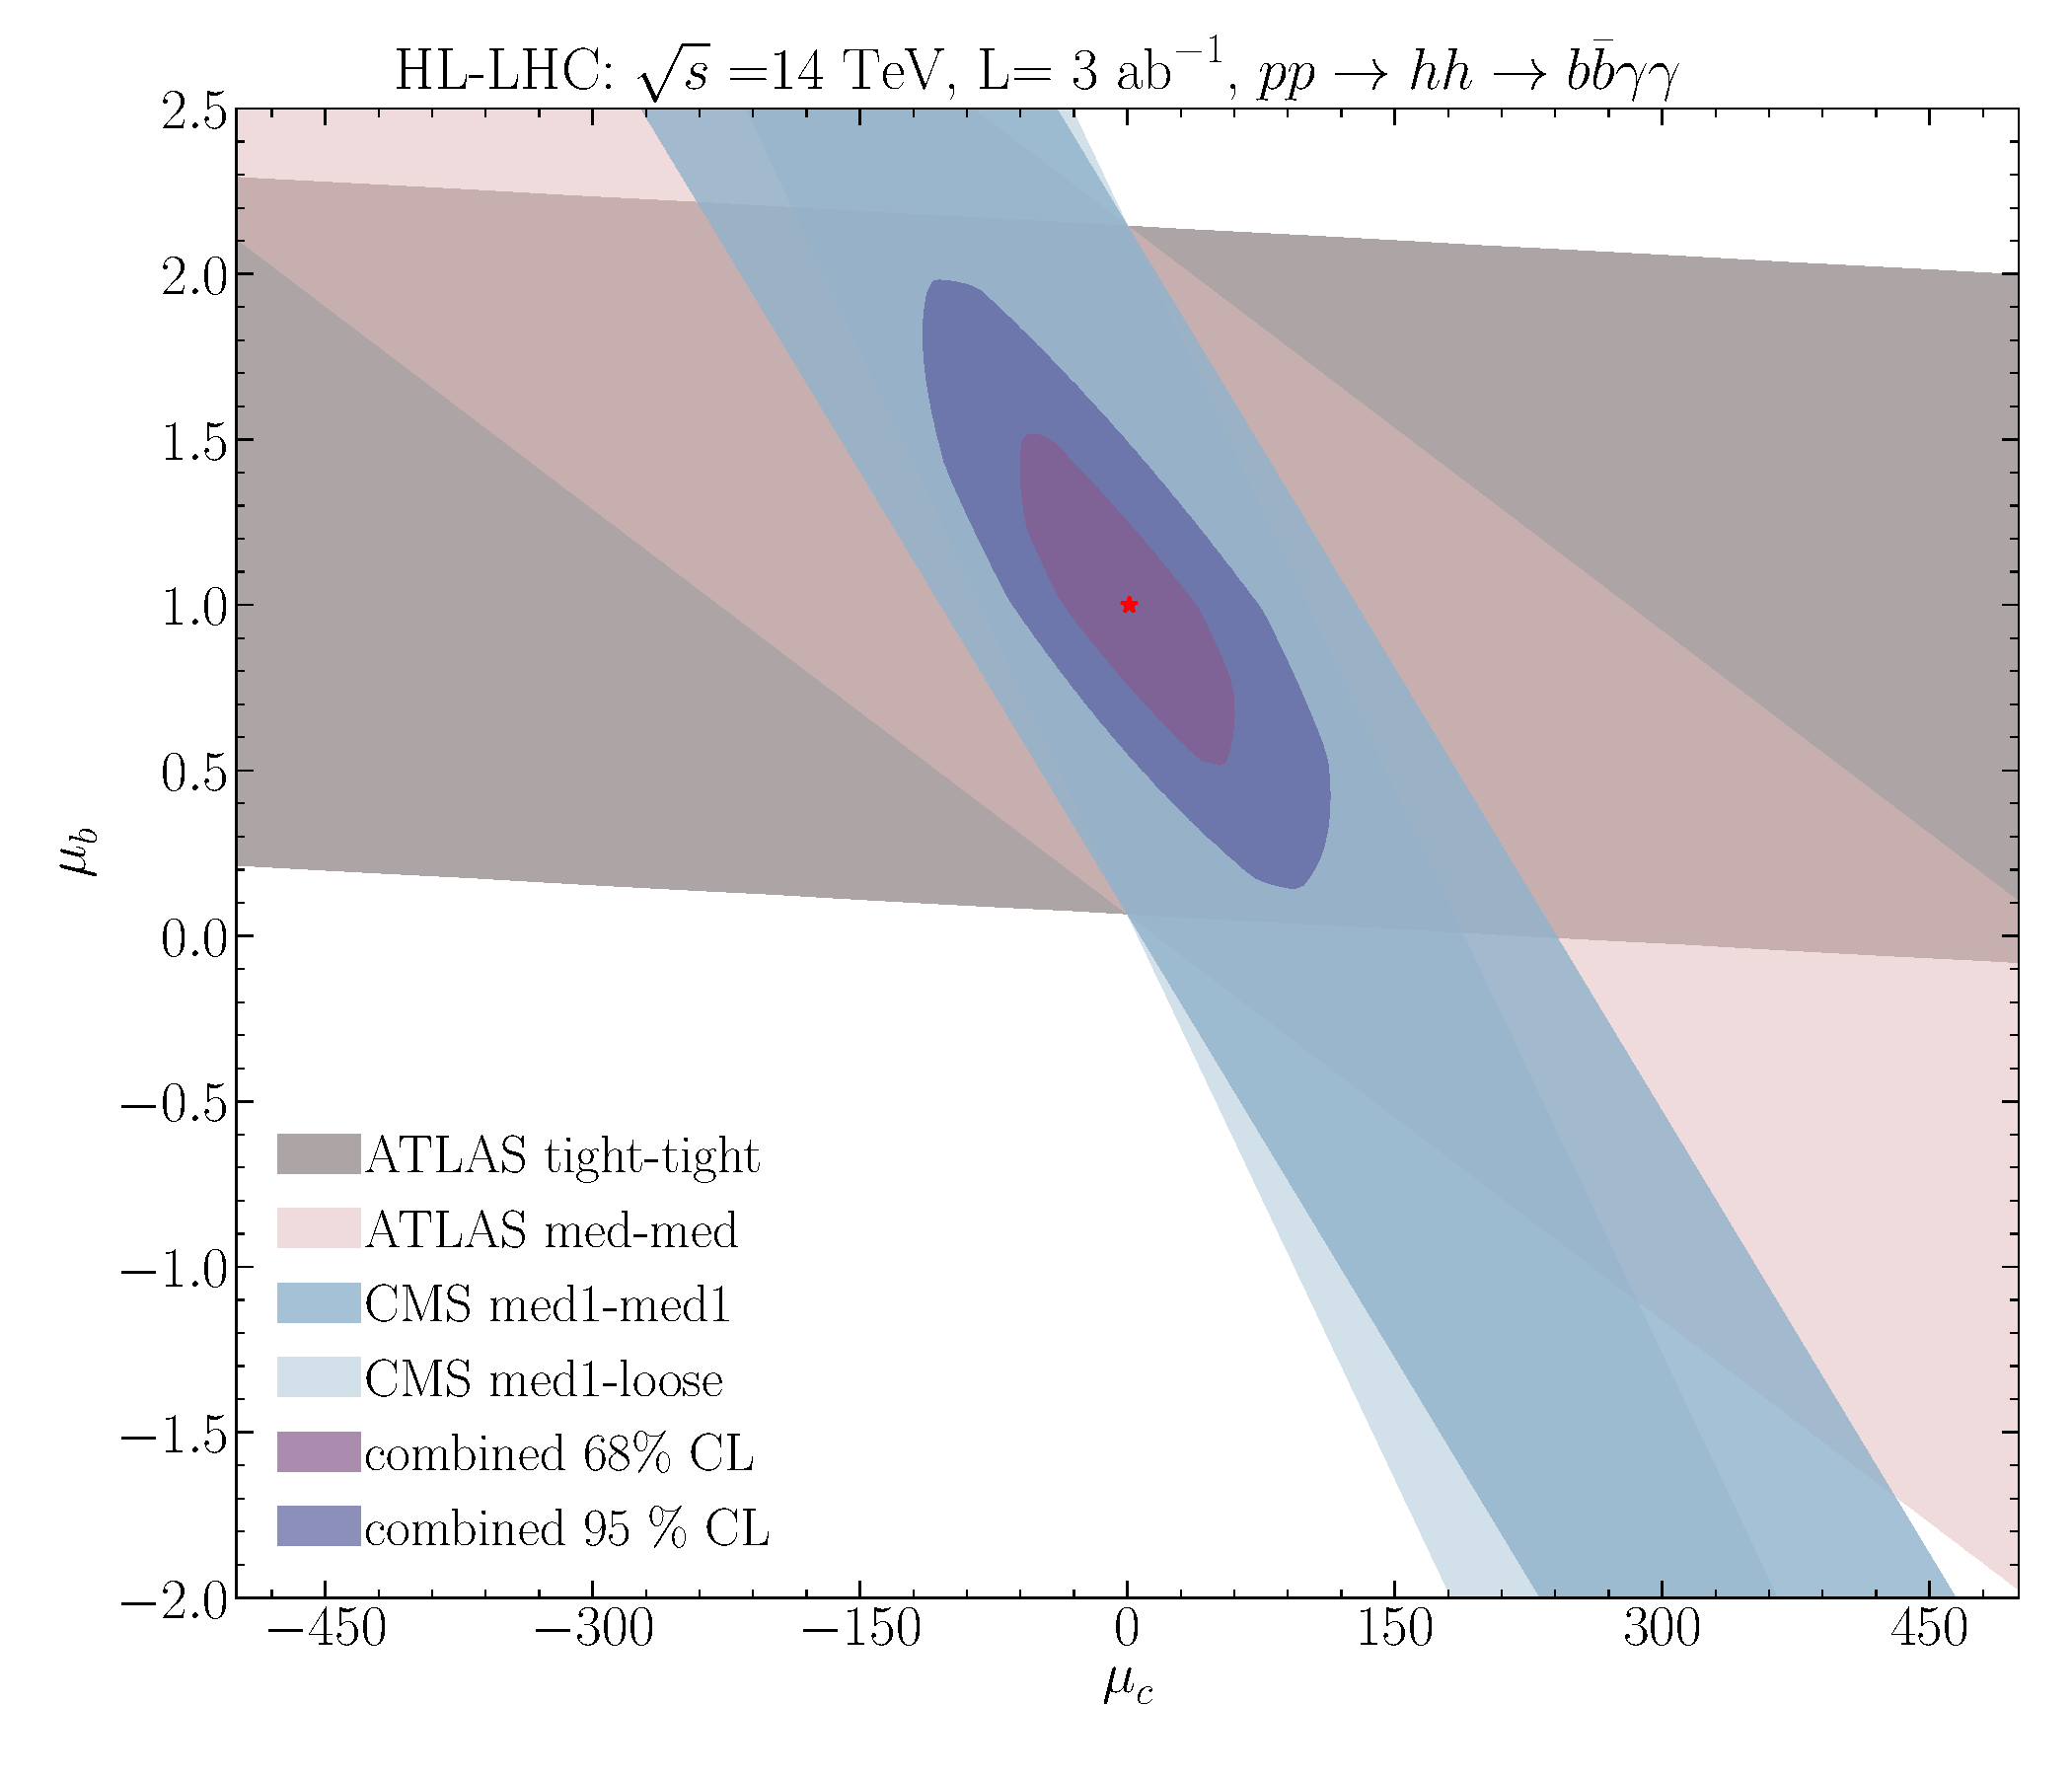
\includegraphics[width = 0.75\textwidth]{./fig/muc_mub_unellepse}
%	\caption{The  95 \% CL contours of $\mu_b$ vs $\mu_c$, obtained from fitting of the signal strength for several CMS and ATLAS $b$-tagging working points. Their combination with the 68\% and 95\% CL upper limits on $\mu_b$ and $\mu_c$ are shown.}
%	\label{bworkingpoints}
%\end{figure}
%One~$b$-tagging working point could only constrain either~$ \mu_b$ or~$\mu_c$. In order to resolve the flat direction several $b$-tagging working points~$\left(\epsilon_{c/b}^{\text{$b$-tag}} \right)^2$ are needed. This is illustrated in fig.~\ref{bworkingpoints}, where the working points fitting contours are combined  using Fisher's method~\cite{heard2018choosing}. We thus obtain an upper projected limit on the charm final state signal strength after profiling over~$\mu_b$,
%\begin{equation}
%	\mu_c(\mathrm{up}) = 36.6 \;(\text{68\% CL})\,, \, \;\;\;\; \,  \mu_c(\mathrm{up}) = 74.8 \;(\text{95\% CL})\,.
%\end{equation}
%However, the obtained sensitivity is not sufficient to set any better limits at 95\% CL than the existing ones (or projected ones in other  channels) for the Yukawa coupling modifiers~$\kappa_c$, and~$\kappa_s$. Instead, we can improve on them by introducing $c$-tagging working points~$(\epsilon_{c/b}^{\text{$c$-tag}})^2$
%\begin{equation}
%	\left( \epsilon_{c/b}^{\text{$c$-tag}}\right)^2 = \frac{\epsilon_{c1}  \epsilon_{c2} }{\epsilon_{c \to b,1} \epsilon_{c \to b,2}}\,,
%\end{equation}
%mixed with the  $b$-tagging ones. We denoted  the contamination of $c$-jets with $b$-jets by $\epsilon_{c \to b}$.  For mixed tagging,  the signal strength estimator becomes
%\begin{equation}
%	\hat \mu = \frac{\sigma_{hh}\, \mathcal B_b \,\epsilon_{b1}\,\epsilon_{b2} \, \epsilon_f+\sigma_{hh}\, \mathcal B_c  \,\epsilon_{c1}\,\epsilon_{c2} \,\epsilon_f }{\sigma_{hh}^{\SM}\, \mathcal B_b^{\SM}\, \epsilon_{b1}\,\epsilon_{b2}
%		+\sigma_{hh}^{\SM}\, \mathcal B_c^{\SM}\, \epsilon_{c1}\,\epsilon_{c2}
%	} \,,
%\end{equation}
%where now $\epsilon_{b}$ is either $\epsilon_{b}$ or $\epsilon_{c\to b}$  and $\epsilon_{c}$ either $\epsilon_{c}$ or $\epsilon_{b\to c}$.
%This simplifies to
%\begin{equation}
%	\hat \mu  = \frac{\mu_b+0.05\,\epsilon_{c/b}^2\,\mu_c}{1+0.05\,\epsilon_{c/b}^2}\, \epsilon_f\,.
%\end{equation}
%The working point~$\epsilon_{c/b}^2$ could be the $b$-tagging or $c$-tagging working point.
%Assuming that $c$-tagging and $b$-tagging are uncorrelated, and working with the methods discussed in~\cite{Perez:2015aoa,Perez:2015lra}, i.e.~combining the ATLAS medium cuts (med.) for $b$-tagging with the $c$-tagging working points in order to break the degeneracy, we could improve the 95\% CL sensitivity on $\mu_c$.
%We start by the $c$-tagging working point used by the ATLAS collaboration in Run I searches for top squarks decays to charm and neutralino~\cite{Aad:2015gna,ATLAS-CONF-2013-063}, which we refer to as $c$-tagging I.
%Further $c$-tagging working points from the HL-LHC upgrade are used: with the expected insertable B-layer (IBL) sub-detector that is to be installed during the ATLAS HL-LHC upgrade~\cite{Capeans:1291633,ATL-PHYS-PUB-2015-018}, the new $c$-tagging II and III points, as illustrated in table~\ref{ctag_wp},
%can be identified. In fig.~\ref{bounds_2ndgen1_btag}  we used them to obtain in combination with the ATLAS med $b$-tagging expected 95\% CL upper limits on~$\mu_c$ for the HL-LHC from an analysis of the final state~$b\bar{b}\gamma\gamma$.
%\begin{table}
%	\centering
%	\begin{tabular}{cccc}
%		\toprule
%		$c$-tagging working point	&$\epsilon_{c}$	& $\epsilon_{c \to b}$ & $\mu_c(\mathrm{up})$ 95\% CL  \\
%		\midrule
%		$c$-tag I ~\cite{Aad:2015gna,ATLAS-CONF-2013-063}
%		& $19\%$ & $13 \%$ & $ 10.1$\\
%		$c$-tag II ~\cite{Capeans:1291633,ATL-PHYS-PUB-2015-018}
%		& $30\%$ & $20 \%$ & $ 8.2$\\
%		$c$-tag III ~\cite{Capeans:1291633,ATL-PHYS-PUB-2015-018}
%		& $50\%$ & $20 \%$ & $ 3.8$\\
%		\bottomrule
%	\end{tabular}
%	\caption{The $c$-tagging working points with the expected 95\% CL upper limit~(sensitivity) of $\mu_c$ obtained after profiling over $\mu_b$. }
%	\label{ctag_wp}
%\end{table}
%%
%%
%%
%%
%Fitting  signal strengths with varying $\kappa_c$,  $\kappa_s$ for charm and bottom final states (\textit{cf.} eq.~\eqref{modelmu}) for constructing the likelihood $\mathscr{L}(\kappa_c,\kappa_s)$, we can set limits from the anticipated charm tagging working points as shown in fig.~\ref{bounds_2ndgen1}.
%\begin{figure}[!t]
%	\centering
%	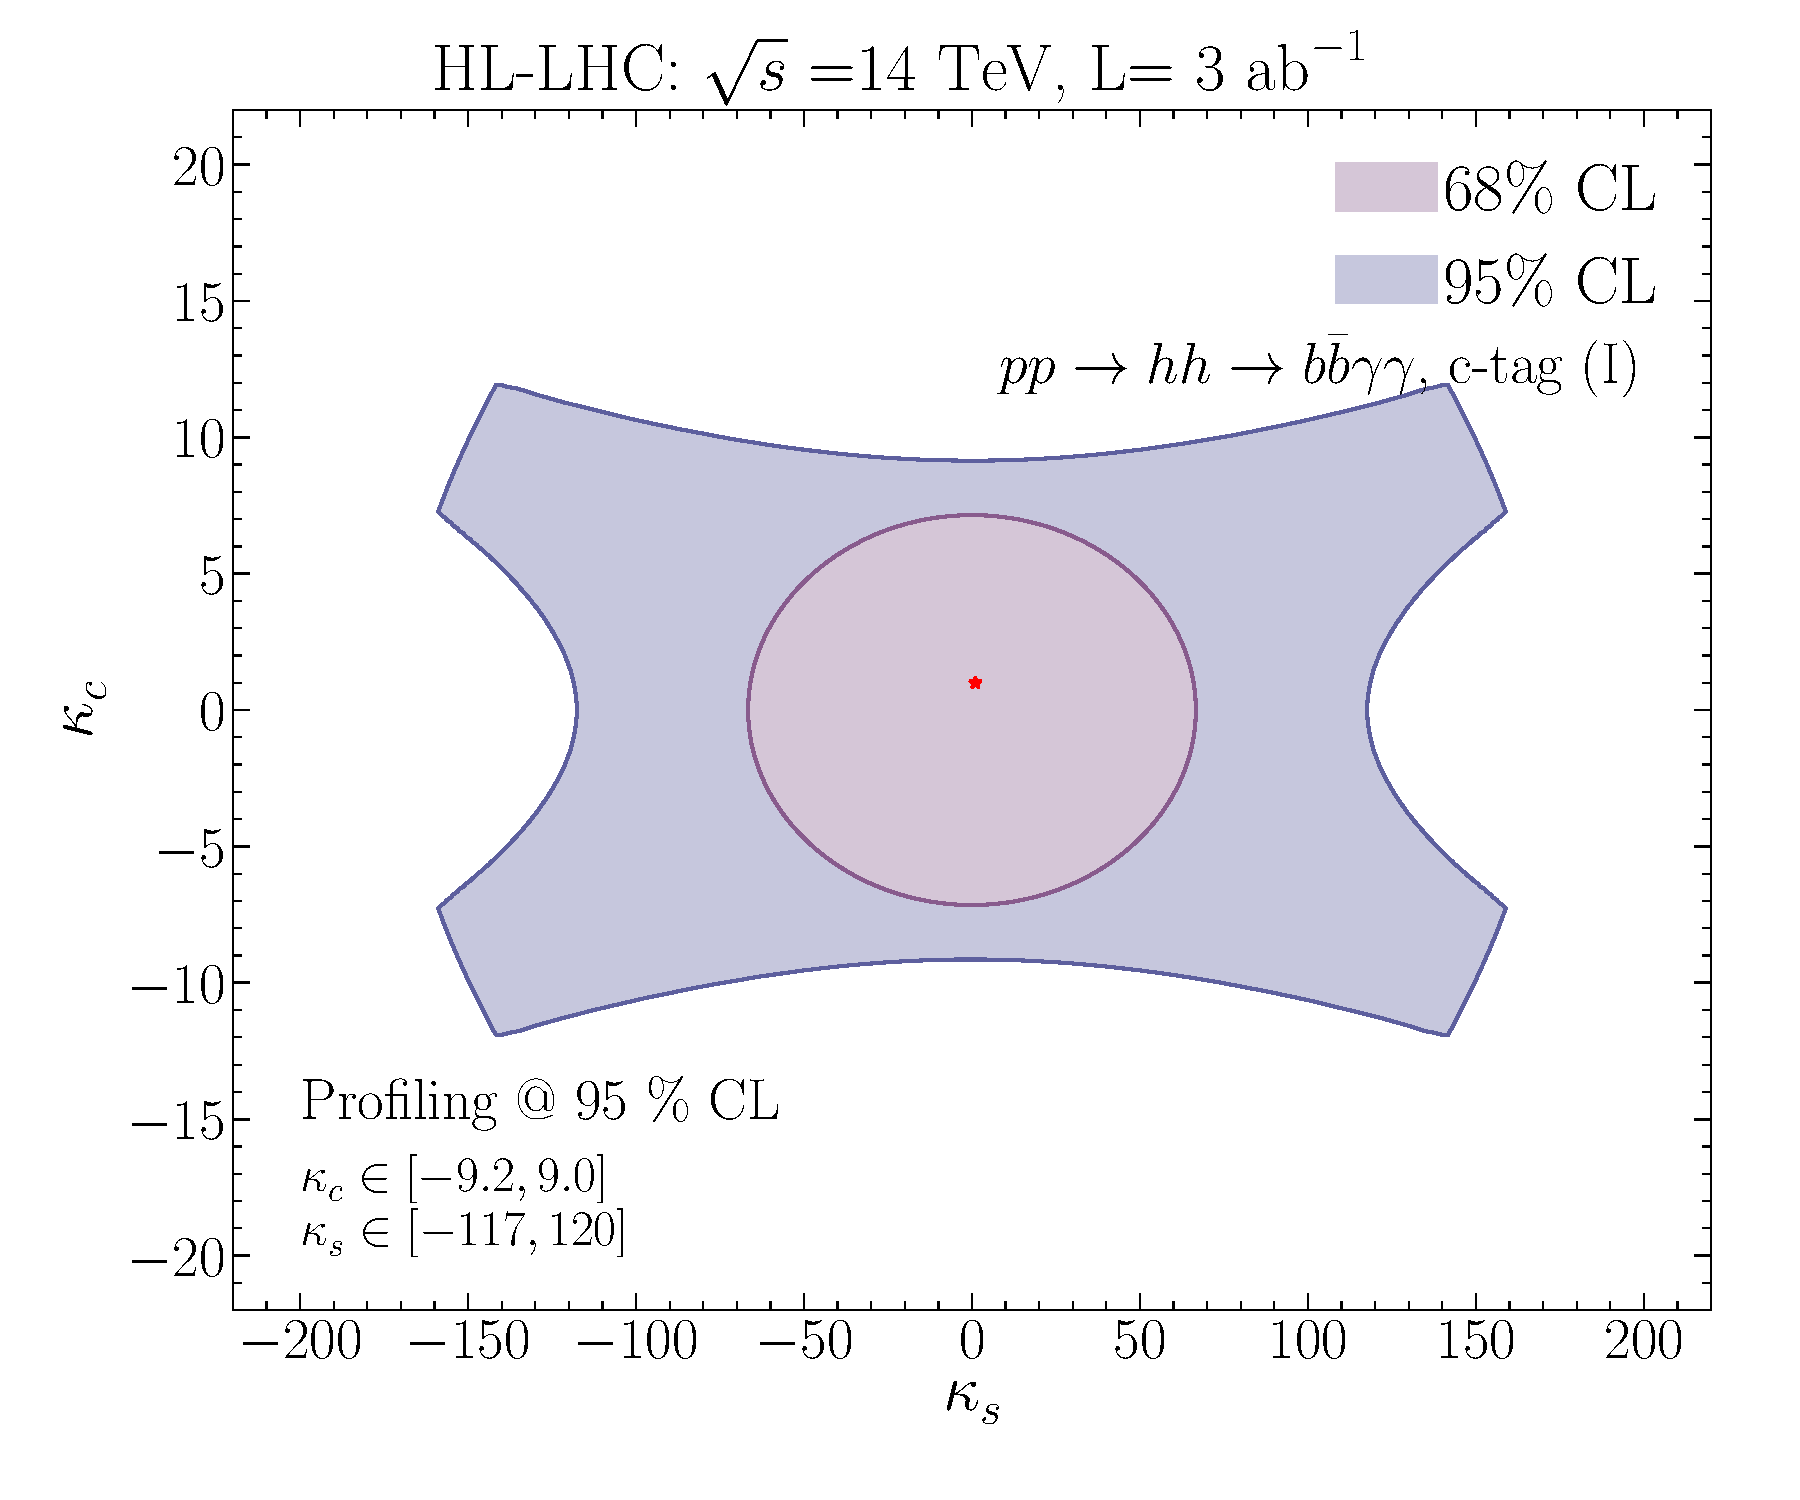
\includegraphics[width = 0.49\textwidth]{./fig/2nd_gen_exclusion_ctag1}
%	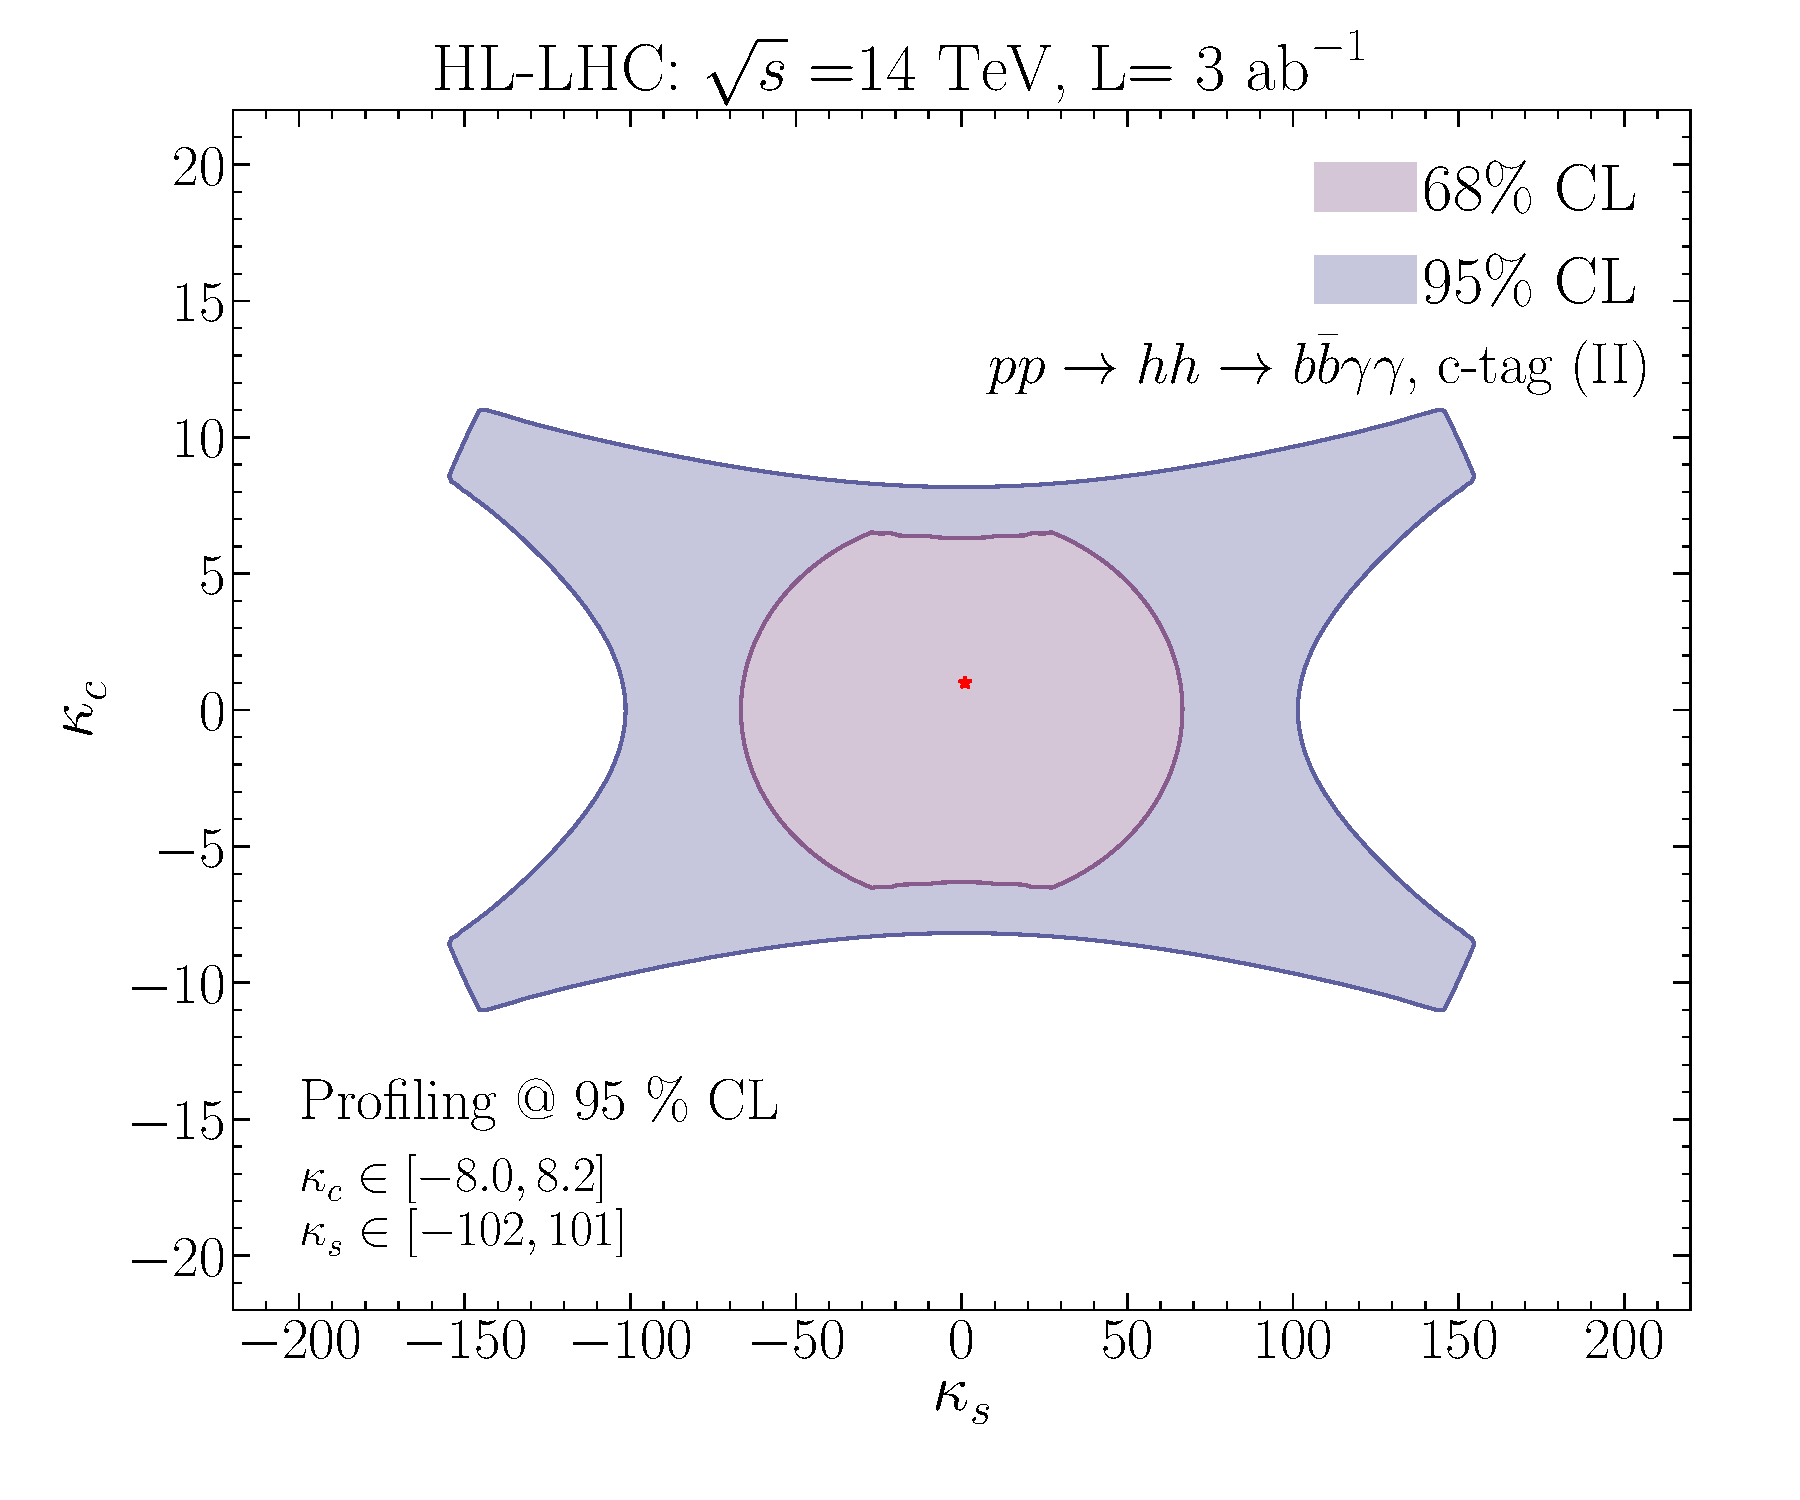
\includegraphics[width = 0.49\textwidth]{./fig/2nd_gen_exclusion_ctag2}
%	\centering
%	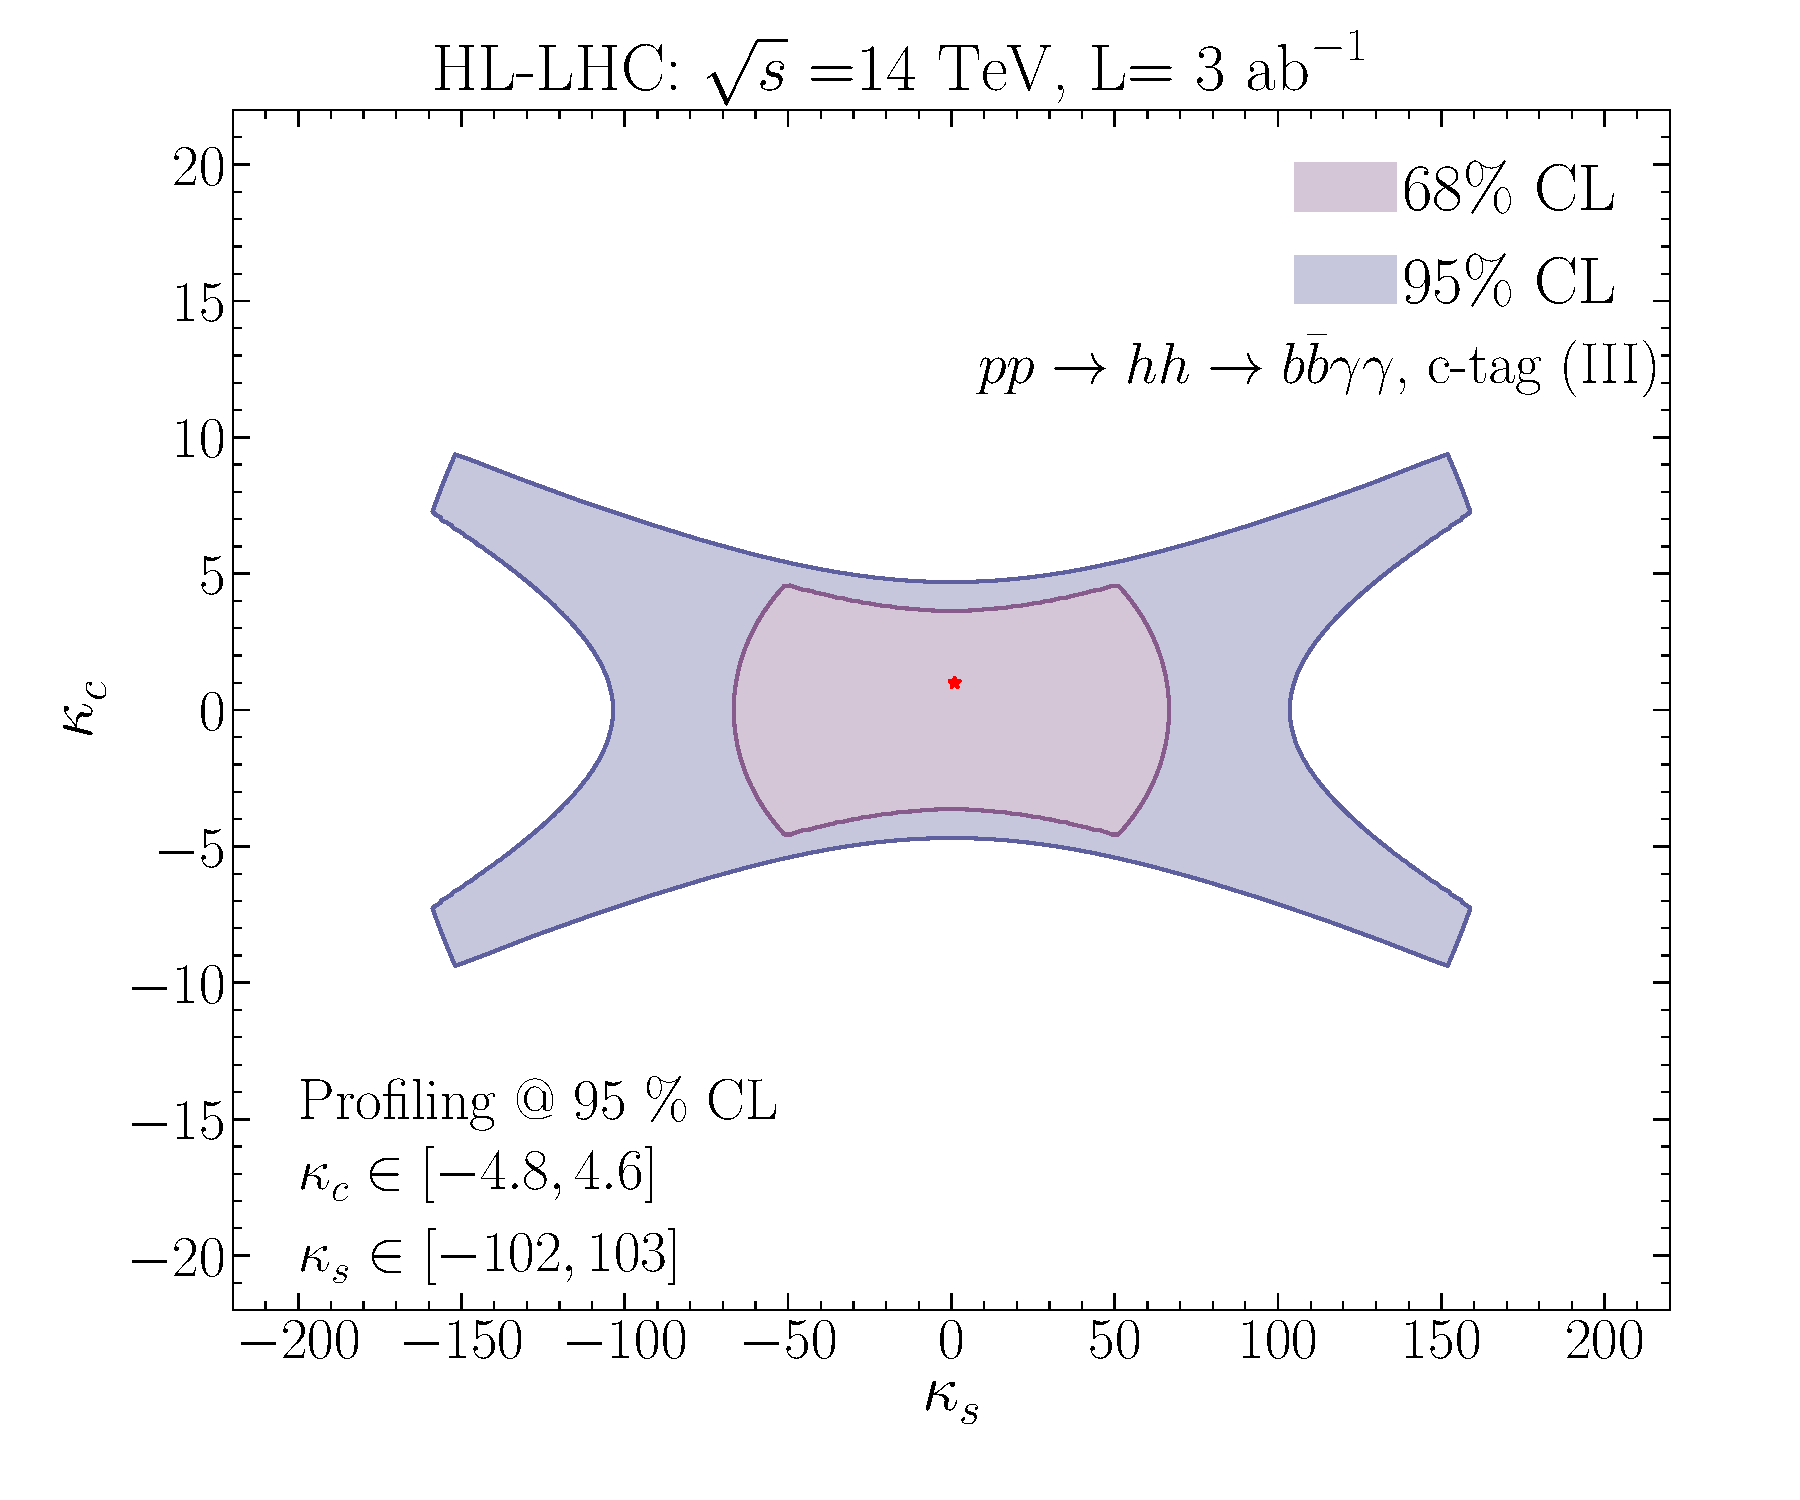
\includegraphics[width = 0.49\textwidth]{./fig/2nd_gen_exclusion_ctag3}
%	\caption{The expected sensitivity likelihood contours at 68\% CL and 95\% CL for an integrated luminosity $L=3000\text{ fb}^{-1}$ for modified second generation quark Yukawa couplings, using the c-tagging I (\textit{upper pannel, left}), II (\textit{upper pannel, right}) and III (\textit{lower pannel}) working points. }
%	\label{bounds_2ndgen1}
%\end{figure}
%These projected limits are an improvement compared to the current direct bound and prospects for HL-LHC, particularly for charm quark Yukawa modifications~\cite{Perez:2015aoa,Perez:2015lra}.
%Again, it should be kept in mind that the bounds on $\kappa_q$ do not just correspond to the scaling of the Yukawa coupling, but also to the new coupling $g_{hhq\bar{q}}$ arising in SMEFT.
%%%%%%%%%%%%%%%%%%%%%%%%%%%%
%
%%%%%%%%%%%%%%%%%%%%%%%%%%%%%%%%%%%%%%%%%%%%%%%%%
%\section{Conclusion \label{sec:conclusion}}
%The couplings to the first and second generation fermions remain among the less well measured couplings of the Higgs boson.
%In this paper we investigated the possibility of measuring light quark Yukawa couplings in Higgs pair production.
%For enhanced Yukawa couplings of the first generation quarks, we found that limits can be set when considering
%quark annihilation with subsequent decay of the Higgs boson pair to $b\bar{b}\gamma\gamma$. In an effective theory description with dimension 6 operators that modify the quark Yukawa couplings,
%there exists also a coupling of two Higgs bosons to two fermions. This coupling increases the Higgs pair production cross section and hence allows to set bounds on the light quark Yukawa coupling modifications.
%For the HL-LHC we found a sensitivity of $|\kappa_u| \lesssim 1170 $ and $|\kappa_d| \lesssim 850 $, \textit{cf}.~fig.~\ref{bounds_1stgen}, which is comparable to the sensitivity of other channels that can directly probe the light quark Yukawa couplings though being weaker than the results from a global fit. Further improvements could be possible with a more dedicated analysis.
%We note though that the bounds we find stem mostly
%due to the diagram involving the coupling of two Higgs bosons to two quarks, as we showed explicitly also by considering a non-linear effective
%theory in which the coupling of one and two Higgs boson to fermions are uncorrelated.
%This channel can hence also be used to distinguish between a linear vs non-linear Higgs EFT hypothesis in the light quark sector.
%The LHC experiments should hence consider the Higgs pair production process in addition to other channels for probing the light quark Yukawa couplings.
%\par
%For the second generation quarks we found that at the HL-LHC in the di-Higgs channel we will be able to set competitive bounds on the
%charm Yukawa coupling if final states with tagged charm quarks are considered.
%We were in particularly considering the final state $c\bar{c}\gamma\gamma$, in which we found a sensitivity of $|\kappa_c| \lesssim 5$ and $|\kappa_s | \lesssim 100 $, \textit{cf.}~fig.~\ref{bounds_2ndgen1}, where the first prospective limit is comparable to the prospects from charm tagging in the $Vh$ channel \cite{Perez:2015lra}.
%
%%%%%%%%%%%%%%%%%%%%%%%%%%%%%%%%%%%%%%%%%%%%%%%%%
%
%%%%%%%%%%%%%%%%%%%%%%%%%%%%%%%%%%%%%%%%%%%%%%%%%%
%%\appendix
%%%%%%%%%%%%%%%%%%%%%%%%%%%%%%%%%%%%%%%%%%%%%%%%%%
%%\section{Parameter values as used in the analysis \label{app:pythia}}
%%In this appendix, we give the input parameters for masses, widths, and couplings as used in the \textsc{Pythia} simulation, see table~\ref{pp}. The collider input is given in table~\ref{cp} and the parton shower parameters in table~\ref{pyp}.
%%\begin{table}[!htpb]
%%	\centering
%%	\begin{tabular}{ccc}
%%		\toprule
%%		Parameter	     & value                    & notes  \\
%%		\midrule
%%		$ m_h$          & \SI{125.25}{\GeV}      & \\
%%		$\Gamma_h$      &\SI{0.013}{\GeV}         &  SM value, changes with $\kappa_f$\\
%%		$v$             & \SI{246.2}{\GeV}      &   \\
%%		$m_W$           & \SI{80.397}{\GeV}       &  \\
%%		$m_Z$           & \SI{91.1876}{\GeV}       &   \\
%%		$\Gamma_W$      & \SI{2.0886}{\GeV}        & \\
%%		$\Gamma_Z$      & \SI{2.4958}{\GeV}        & \\
%%		$m_t$           & \SI{173.21}{\GeV}      & pole mass \\
%%		$m_b$           & \SI{4.18}{\GeV}        & \multirow{2}{*}{$\bar{\text{MS}}$ mass at $\mu = 2$ \si{\GeV} }\\
%%		$m_c$           & \SI{1.27}{\GeV}        &  \\
%%		$m_s$           & \SI{96.0}{\MeV}       & \\
%%		$m_u$           & \SI{2.20}{\MeV}        & \\
%%		$m_d$           & \SI{4.70}{\MeV}        & \\
%%		$\alpha_s(m_Z)$ & $0.118$                 & \\
%%		$(hc)^2$            &\SI{3.894e11}{\femto\barn \per \GeV\squared} & conversion from $\GeV^2$ to $\femtobarn$ \\
%%		\bottomrule
%%	\end{tabular}
%%	\caption{The input parameters used in this work, all taken from the PDG \cite{Tanabashi:2018oca}. }
%%	\label{pp}
%%\end{table}
%%
%%\begin{table}[!htpb]
%%	\centering
%%	\begin{tabular}{ccc}
%%		\toprule
%%		Parameter	& value & description  \\
%%		\midrule
%%		PDG ID's of initial states  & (2212,2212)  &$pp$ collision\\
%%		$\sqrt{s}$      & \SI{14}{\TeV} &  centre of mass energy\\
%%		$L$             & \SI{3}{\per\atto\barn} &  integrated luminosity \\
%%		LHAPDF ID     & $262000$   &  NNPDF30 LO          \\
%%		\bottomrule
%%	\end{tabular}
%%	\caption{The collider parameters used in this work for the HL-LHC. }
%%	\label{cp}
%%\end{table}
%%
%%\begin{table}[!htpb]
%%	\centering
%%	\begin{tabular}{ccc}
%%		\toprule
%%		Parameter	& value & description  \\
%%		\midrule
%%		\texttt{  MSTU(112)} & 5   &  5-flavour scheme. \\
%%		\texttt{  MSTP(48) } & 1  & Top quark decay before fragmentation. \\
%%		\texttt{  MSTP(61)}  & 1 & Turn on initial state radiation.\\
%%		\texttt{  MSTP(71)}  & 1 & Turn on final state radiation.\\
%%		\texttt{MSTJ(41)}  & 1 & Turn off QED bremsstrahlung.\\
%%		\texttt{MSTP(81)}  & 1 & Multiple interaction on. \\
%%		\texttt{MSTP(111)}  & 2 & Allow fragmentation and decay. \\
%%		\texttt{MSTP(42)}   & 0 & Turn off  shell boson production. \\
%%		\bottomrule
%%	\end{tabular}
%%	\caption{The values of \textsc{Pythia} 6.4 parameters that are changed compared to the default values.}
%%	\label{pyp}
%%\end{table}